\documentclass{article}
\usepackage{hyperref}
\usepackage{graphicx}
\usepackage{amsmath}
\usepackage{amssymb}
\usepackage{enumerate}
\usepackage{blindtext}
\usepackage{mathtools}
\usepackage[ruled,vlined]{algorithm2e}
\usepackage{mathabx}
\usepackage{bm}
\usepackage{caption}
\usepackage{subcaption}
\usepackage{array}
\usepackage{multirow}
\usepackage{tikz}
\tikzset{
  treenode/.style = {align=center, inner sep=0pt, text centered,
    font=\sffamily},
  arn_n/.style = {treenode, circle, blue, draw=blue, text width=1.5em, very thick},% arbre rouge noir, noeud noir
  arn_r/.style = {treenode, circle, red, draw=red, text width=1.5em, very thick},% arbre rouge noir, noeud rouge
  arn_o/.style = {treenode, circle, orange, draw=orange, text width=1.5em, very thick},
  arn_x/.style = {treenode, rectangle, draw=black,
    minimum width=0.5em, minimum height=0.5em}% arbre rouge noir, nil
}
    \newcolumntype{P}[1]{>{\centering\arraybackslash}p{#1}}
    \newcolumntype{M}[1]{>{\centering\arraybackslash}m{#1}}
\usepackage{stackengine}
    \newcommand\xrowht[2][0]{\addstackgap[0.5\dimexpr#2\relax]{\vphantom{#1}}}
\addtolength{\oddsidemargin}{-.875in}
\addtolength{\evensidemargin}{-.875in}
\addtolength{\textwidth}{1.75in}
\addtolength{\topmargin}{-.875in}
\addtolength{\textheight}{1.75in}
\renewcommand{\thealgocf}{S\arabic{algocf}}
% \renewcommand{\thelyxalgorithm}{A\arabic{algorithm}}
\renewcommand{\theequation}{S\arabic{equation}}
\renewcommand{\thefigure}{S\arabic{figure}}
\renewcommand{\thesection}{S\arabic{section}}
\renewcommand{\thetable}{S\arabic{table}}
\DeclareMathOperator*{\argmin}{argmin}
\DeclareMathOperator*{\argmax}{argmax}
\newcolumntype{N}{@{}m{0pt}@{}}
\usepackage{natbib}
\usepackage{amsfonts}
\newcommand{\tickYes}{\checkmark}
\usepackage{pifont}
\newcommand{\tickNo}{\hspace{1pt}\ding{55}}
\newcommand{\tickHalfYes}{\checkmark\!\!\!\raisebox{0.4 em}{\tiny$\smallsetminus$}}

%usepackage{subfiles} % Best loaded last in the preamble

\title{Supplementary Information of distAngsd: Novel and Fast Phylogeny Inference Methods that Allow for Uncertainties Introduced by Sequencing and Low Coverage}
\author{Lei Zhao,  Rasmus Nielsen, and Thorfinn Sand Korneliussen}

\date{ }

\begin{document}

\maketitle
\section{Genotype Likelihood}\label{sec:GL}
Genotype likelihood is the likelihood function $\mathrm{GL}_i^s(\cdot)$ of the true genotype $g$ at a specific site $s$ in the $i$'th sample, given the observed reads at site $s$ in sample $i$ can be denoted as a vector $\vec{o}_i^s$, i.e.,
\begin{align*}
    \mathrm{GL}_i^s(g)=L(g|\vec{o}_i^s)=\mathrm{P}(\vec{o}_i^s|g),
\end{align*}
The detailed forms of the genotype likelihoods vary based on different models (refs). The GATK form of diploid genotype likelihood (Equation \ref{eq:GATKGL}) is used for simulation inference, while the bcftools calultes genotype likelihoods in another form (Equation \ref{eq:bamGL}), which are present in the .vcf file and are used for real data inference in this work.
\begin{align}
\widetilde{\mathrm{GL}}_i^s(g)=\prod_{k=1}^{\#\mathrm{reads}}\mathrm{P}(r_k|g),\label{eq:GATKGL}
\end{align}
where
\begin{align*}
\mathrm{P}(r_k=l|g=ij) = \left\{\begin{array}{ll}
     1-e_k, & {\rm If\hspace{0.1cm}} l=i=j,  \\
     \frac{e_k}{3}, & {\rm If\hspace{0.1cm}} l\neq i {\hspace{0.1cm}\rm and\hspace{0.1cm}} l\neq j, \\
     \frac{1}{2}-\frac{e_k}{3}, &  {\rm Otherwise,}
\end{array}\right.,
\end{align*}
 and $i$, $j$ and $l$ are nucleotides, and $e_k$ is the base calling error of the $k$'th read at the focal base. $\mathrm{P}(r_k=l|g=ij)$ represents the probability of the $k$'th read of a particular nucleotide is $l$ given the true genotype is $ij$.
 \begin{align}
 \widetilde{\mathrm{GL}}_i^s(g=ij)=\left\{\begin{array}{cc}
      \prod\limits_{l\neq i}\prod\limits_{k=1}^{n_l}\left[\frac{\sum\limits_{m=k}^n\left(\begin{array}{c}
           n  \\
           m 
      \end{array}\right)e_{l,k}^m(1-e_{l,k})^{n-m}}{\sum\limits_{m=k-1}^n\left(\begin{array}{c}
           n  \\
           m 
      \end{array}\right)e_{l,k}^m(1-e_{l,k})^{n-m}}\right]^{0.97\times 0.83^{k-1}+0.03} & i=j,  \\
      \left(\begin{array}{c}
           n_i+n_j  \\
           n_i
      \end{array}\right)\left(\frac{1}{2}\right)^{n_i+n_j}\prod\limits_{l\neq i,j}\prod\limits_{k=1}^{n_l}\left[\frac{\sum\limits_{m=k}^n\left(\begin{array}{c}
           n  \\
           m 
      \end{array}\right)e_{l,k}^m(1-e_{l,k})^{n-m}}{\sum\limits_{m=k-1}^n\left(\begin{array}{c}
           n  \\
           m 
      \end{array}\right)e_{l,k}^m(1-e_{l,k})^{n-m}}\right]^{0.97\times 0.83^{k-1}+0.03}& i\neq j, 
 \end{array}\right. \label{eq:bamGL}
 \end{align}
 where $i$, $j$ and $l$ are nucleotides, $n$ is the read depth of the focal base, $n_i$ is the counts of reads that calls nucleotide $i$ at the focal base, and $e_{l,k}$ is the base calling error of the $k$'th read that calls nucleotide $l$ at the focal base. The series of the calling errors that calls nucleotide $l$ at the focal base $\{e_{l,k}\}_{k=1}^{n_l}$ should be ordered in an ascend sense in the bam form genotype likelihood definition.
 
In practice, both forms of genotype likelihoods (i.e, Equation \ref{eq:GATKGL} and Equation \ref{eq:bamGL}) will be rescaled as follows to enhance calculation stability,
\begin{align*}
\mathrm{GL}_i^s(g=ij) = \frac{\widetilde{\mathrm{GL}}_i^s(g=ij)}{\max_{g}\widetilde{\mathrm{GL}}_i^s(g)},
\end{align*}
Throughout this work, we assume the applied genotype likelihoods make perfect sense, i.e., no error will be introduced by the genotype likelihood calculations. But we do believe such value may need further re-calibration.

\section{Expectation-Maximization Algorithm} \label{sec:EM}
Both distAngsd-geno and distAngsd-nuc apply the Expectation-Maximization Algorithm (EM Algorithm) to obtain an estimation the joint distribution matrix of genotypes, ${\bf M}$ or the joint distribution matrix of sampled nucleotides for both samples, ${\bf N}$, given the observations . ${\bf M}$ is a $10\times 10$ matrix, whose elements are denoted as ${\bf M}(g_1,g_2)$, representing the joint probability that the true genotypes are $g_1$ (e.g., AA) and $g_2$ (e.g. AC) at the same site in sample $1$ and $2$, respectively. Similarly, ${\bf N}$ is a $4\times 4$ matrix with each element ${\bf N}(n_1,n_2)$ denoting the joint distribution of sampled nucleotides which derive the randomly chosen read pairs from the sample pair at the same site.

The brief idea of EM algorithm can be put as the following equations,
\begin{align}
l\left({\bf M}|\vec{o}_1,\vec{o}_2\right)=&\log\mathrm{P}\left(\vec{o}_1,\vec{o}_2|{\bf M}\right)\nonumber\\
=&\log\prod_{s=1}^{\#\mathrm{sites}}\mathrm{P}\left(\vec{o}_1^s,\vec{o}_2^s|{\bf M}\right)\nonumber\\
=&\sum_{s=1}^{\#\mathrm{sites}}\log\mathrm{P}\left(\vec{o}_1^s,\vec{o}_2^s|{\bf M}\right)\nonumber\\
=&\sum_{s=1}^{\#\mathrm{sites}}\log\sum_{g_1^s,g_2^s}\mathrm{P}\left(\vec{o}_1^s,\vec{o}_2^s,g_1^s,g_2^s|{\bf M}\right)\nonumber\\
=&\sum_{s=1}^{\#\mathrm{sites}}\log\sum_{g_1^s,g_2^s}\frac{\mathrm{P}\left(\vec{o}_1^s,\vec{o}_2^s,g_1^s,g_2^s|{\bf M}\right)}{\mathrm{P}\left(g_1^s,g_2^s|{\bf M}_{t},\vec{o}_1,\vec{o}_2\right)}\times \mathrm{P}\left(g_1^s,g_2^s|{\bf M}_{t},\vec{o}_1,\vec{o}_2\right)\nonumber\\
\geq&\sum_{s=1}^{\#\mathrm{sites}}\sum_{g_1^s,g_2^s}\log\mathrm{P}\left(\vec{o}_1^s,\vec{o}_2^s,g_1^s,g_2^s|{\bf M}\right)\times \mathrm{P}\left(g_1^s,g_2^s|{\bf M}_{t},\vec{o}_1,\vec{o}_2\right)-C \nonumber\\
=&\sum_{s=1}^{\#\mathrm{sites}}\mathrm{E}_{{\bf M}_{t},\vec{o}_1,\vec{o}_2}\left[\log\mathrm{P}\left(\vec{o}_1^s,\vec{o}_2^s,g_1^s,g_2^s|{\bf M}\right)\right]-C \nonumber\\
\triangleq& f({\bf M}|{\bf M}_t,\vec{o}_1,\vec{o}_2), \label{eq:distAngsd-genoEM}
\end{align}
where the equality can be achieved when ${\bf M}={\bf M}_t$, and $\mathrm{E}_{{\bf M}_{t},\vec{o}_1,\vec{o}_2}[\cdot]\triangleq \mathrm{E}[\cdot|{\bf M}_{t},\vec{o}_1,\vec{o}_2]$. $g_i^s$ is the true genotype at site $s$ of the $i$'th sample. $\vec{o}_i$ is the observed data from sample $i$, while $\vec{o}_i^s$ is all the observed nucleotide reads at site $s$ from sample $i$.

\begin{align}
&l\left({\bf N}|\vec{o}_1,\vec{o}_2\right) \nonumber\\
=&\log\mathrm{P}\left(\vec{o}_1,\vec{o}_2|{\bf N}\right) \nonumber\\
=&\sum_{s=1}^{\#\mathrm{sites}}\log\mathrm{P}\left(\vec{o}_1^s,\vec{o}_2^s|{\bf N}\right)\nonumber\\
=&\sum_{s=1}^{\#\mathrm{sites}}\frac{1}{\#\mathrm{read}_1^s\times\#\mathrm{read}_2^s}\log\prod_{r_1=1}^{\#\mathrm{read}_1^s}\prod_{r_2=1}^{\#\mathrm{read}_2^s}\mathrm{P}\left(o_1^{s,r_1},o_2^{s,r_2}|{\bf N}\right)\nonumber\\
=&\sum_{s=1}^{\#\mathrm{sites}}\frac{1}{\#\mathrm{read}_1^s\times\#\mathrm{read}_2^s}\sum_{r_1=1}^{\#\mathrm{read}_1^s}\sum_{r_2=1}^{\#\mathrm{read}_2^s}\log\mathrm{P}\left(o_1^{s,r_1},o_2^{s,r_2}|{\bf N}\right)\nonumber\\
=&\sum_{s=1}^{\#\mathrm{sites}}\frac{1}{\#\mathrm{read}_1^s\times\#\mathrm{read}_2^s}\sum_{r_1=1}^{\#\mathrm{read}_1^s}\sum_{r_2=1}^{\#\mathrm{read}_2^s}\log\sum_{n_1^{s,r_1},n_2^{s,r_2}}\mathrm{P}\left(o_1^{s,r_1},o_2^{s,r_2},n_1^{s,r_1},n_2^{s,r_2}|{\bf N}\right)\nonumber\\
=&\sum_{s=1}^{\#\mathrm{sites}}\frac{\sum\limits_{r_1=1}^{\#\mathrm{read}_1^s}\sum\limits_{r_2=1}^{\#\mathrm{read}_2^s}\log\sum\limits_{n_1^{s,r_1},n_2^{s,r_2}}\frac{\mathrm{P}\left(o_1^{s,r_1},o_2^{s,r_2},n_1^{s,r_1},n_2^{s,r_2}|{\bf N}\right)}{\mathrm{P}\left(n_1^{s,r_1},n_2^{s,r_2}|{\bf N}_t,\vec{o}_1,\vec{o}_2\right)}\times \mathrm{P}\left(n_1^{s,r_1},n_2^{s,r_2}|{\bf N}_t,\vec{o}_1,\vec{o}_2\right)}{\#\mathrm{read}_1^s\times\#\mathrm{read}_2^s}\nonumber\\
\geq&\sum_{s=1}^{\#\mathrm{sites}}\frac{\sum\limits_{r_1=1}^{\#\mathrm{read}_1^s}\sum\limits_{r_2=1}^{\#\mathrm{read}_2^s}\sum\limits_{n_1^{s,r_1},n_2^{s,r_2}}\log\mathrm{P}\left(o_1^{s,r_1},o_2^{s,r_2},n_1^{s,r_1},n_2^{s,r_2}|{\bf N}\right)\times \mathrm{P}\left(n_1^{s,r_1},n_2^{s,r_2}|{\bf N}_t,\vec{o}_1,\vec{o}_2\right)}{\#\mathrm{read}_1^s\times\#\mathrm{read}_2^s}-C\nonumber\\
=&\sum_{s=1}^{\#\mathrm{sites}}\frac{\sum\limits_{r_1=1}^{\#\mathrm{read}_1^s}\sum\limits_{r_2=1}^{\#\mathrm{read}_2^s}\mathrm{E}_{{\bf N}_t,\vec{o}_1,\vec{o}_2}\left[\log\mathrm{P}\left(o_1^{s,r_1},o_2^{s,r_2},n_1^{s,r_1},n_2^{s,r_2}|{\bf N}\right)\right]}{\#\mathrm{read}_1^s\times\#\mathrm{read}_2^s}-C \nonumber\\
\triangleq& g({\bf N}|{\bf N}_t,\vec{o}_1,\vec{o}_2),\label{eq:distAngsd-nucEM}
\end{align}
where the equality can be achieved when ${\bf N}={\bf N}_t$, and $\mathrm{E}_{{\bf N}_{t},\vec{o}_1,\vec{o}_2}[\cdot]\triangleq \mathrm{E}[\cdot|{\bf N}_{t},\vec{o}_1,\vec{o}_2]$. $\#\mathrm{read}_i^s$ represents the total read depth at site $s$ of sample $i$. $n_i^{s,r_i}$ and $o_i^{s,r_i}$ are the true sampled nucleotide and the observed nucleotide of the $r_i$th read at the site $s$ of the sample $i$.

The inequalities in Equation \ref{eq:distAngsd-genoEM} and Equation \ref{eq:distAngsd-nucEM} are due to the concave nature of logarithm function (Jensen's Inequality (ref)). Hence, instead of maximize the original $l\left({\bf M}|\vec{o}_1,\vec{o}_2\right)$ (or $l\left({\bf N}|\vec{o}_1,\vec{o}_2\right)$), we can alternatively optimize the its lower bound, i.e., $f({\bf M}|{\bf M}_t,\vec{o}_1,\vec{o}_2)$ (or $g({\bf N}|{\bf N}_t,\vec{o}_1,\vec{o}_2)$), and iteratively update ${\bf M}_t$ (or ${\bf N}_t$) by ${\bf M}_{t+1}=\argmax_{{\bf M}}f$ (or ${\bf N}_{t+1}=\argmax_{{\bf N}}g$), which outlines the procedures of the EM algorithm.
\subsection{Expectation Step}
\begin{align}
&f({\bf M}|{\bf M}_{t},\vec{o}_1,\vec{o}_2)\nonumber\\
=&\sum_{s=1}^{\#\mathrm{sites}}\mathrm{E}_{{\bf M}_{t},\vec{o}_1,\vec{o}_2}\left[\log\mathrm{P}\left(\vec{o}_1^s,\vec{o}_2^s,g_1^s,g_2^s|{\bf M}\right)\right]\nonumber\\
=&\sum_{s=1}^{\#\mathrm{sites}}\mathrm{E}_{{\bf M}_{t},\vec{o}_1,\vec{o}_2}\left[\log\delta_{g_1^s,g_2^s}+\log\mathrm{GL}_1^s(g_1^s)+\log\mathrm{GL}_2^s(g_2^s)\right]\nonumber\\
=&\sum_{g_1,g_2}\sum_{s=1}^{\#\mathrm{sites}}\mathrm{E}_{{\bf M}_{t},\vec{o}_1,\vec{o}_2}\left[u_{g_1,g_2}(s)\right]\left[\log{\bf M}(g_1,g_2)+\log\mathrm{GL}_1^s(g_1)+\log\mathrm{GL}_2^s(g_2)\right],\label{eq:distAngsd-genoEStep}
\end{align}
where $u_{g_1,g_2}(s)=\left\{\begin{array}{cc}
   1,  & g_1^s=g_1, g_2^s=g_2,\\
   0,  & \mathrm{otherwise}.
\end{array}\right.$, and $\mathrm{GL}_i^s(g_i)$ is the genotype likelihood function (see definitions in Section \ref{sec:GL}) of true genotype $g_i$ at site $s$ in sample $i$ ($i=1$ or $2$), and the expectation $\mathrm{E}_{{\bf M}_{t},\vec{o}_1,\vec{o}_2}\left[u_{g_1,g_2}(s)\right]$ can be expressed as follows,
\begin{align*}
    \mathrm{E}_{{\bf M}_{t},\vec{o}_1,\vec{o}_2}\left[u_{g_1,g_2}(s)\right]&=\mathrm{P}\left(g_1^s=g_1, g_2^s=g_2|{\bf M}_{t},\vec{o}_1,\vec{o}_2\right)\\
    &=\frac{\mathrm{P}\left(g_1^s=g_1, g_2^s=g_2,\vec{o}_1,\vec{o}_2|{\bf M}_{t}\right)}{\mathrm{P}\left(\vec{o}_1,\vec{o}_2|{\bf M}_{t}\right)}\\
    &=\frac{\mathrm{P}\left(g_1^s=g_1, g_2^s=g_2,\vec{o}_1,\vec{o}_2|{\bf M}_{t}\right)}{\sum\limits_{g_1,g_2}\mathrm{P}\left(g_1^s=g_1, g_2^s=g_2,\vec{o}_1,\vec{o}_2|{\bf M}_{t}\right)}\\
    &=\frac{{\bf M}_{t}(g_1,g_2)\mathrm{GL}_1^s(g_1)\mathrm{GL}_2^s(g_2)}{\sum\limits_{g_1,g_2}{\bf M}_{t}(g_1,g_2)\mathrm{GL}_1^s(g_1)\mathrm{GL}_2^s(g_2)}
\end{align*}
\begin{align}
&g({\bf N}|{\bf N}_t,\vec{o}_1,\vec{o}_2)\nonumber\\
    =&\sum_{s=1}^{\#\mathrm{sites}}\frac{\sum\limits_{r_1=1}^{\#\mathrm{read}_1^s}\sum\limits_{r_2=1}^{\#\mathrm{read}_2^s}\mathrm{E}_{{\bf N}_t,\vec{o}_1,\vec{o}_2}\left[\log\mathrm{P}\left(o_1^{s,r_1},o_2^{s,r_2},n_1^{s,r_1},n_2^{s,r_2}|{\bf N}\right)\right]}{\#\mathrm{read}_1^s\times\#\mathrm{read}_2^s}\nonumber\\
=&\sum_{s=1}^{\#\mathrm{sites}}\frac{\sum\limits_{r_1=1}^{\#\mathrm{read}_1^s}\sum\limits_{r_2=1}^{\#\mathrm{read}_2^s}\mathrm{E}_{{\bf N}_t,\vec{o}_1,\vec{o}_2}\left[\log\delta_{n_1^{s,r_1},n_2^{s,r_2}}+\log\mathrm{P}(o_1^{s,r_1}|n_1^{s,r_1})+\log\mathrm{P}(o_2^{s,r_2}|n_2^{s,r_2})\right]}{\#\mathrm{read}_1^s\times\#\mathrm{read}_2^s}\nonumber\\
=&\sum_{n_1,n_2}\sum_{s=1}^{\#\mathrm{sites}}\frac{\sum\limits_{r_1=1}^{\#\mathrm{read}_1^s}\sum\limits_{r_2=1}^{\#\mathrm{read}_2^s}\mathrm{E}_{{\bf N}_t,\vec{o}_1,\vec{o}_2}\left[v_{n_1,n_2}(s,r_1,r_2)\right]\left[\log{\bf N}(n_1,n_2)+\log\mathrm{P}(o_1^{s,r_1}|n_1)+\log\mathrm{P}(o_2^{s,r_2}|n_2)\right]}{\#\mathrm{read}_1^s\times\#\mathrm{read}_2^s},\label{eq:distAngsd-nucEStep}
\end{align}
where $v_{n_1,n_2}(s,r_1,r_2)=\left\{\begin{array}{cc}
   1,  & n_1^{s,r_1}=n_1, n_2^{s,r_2}=n_2,\\
   0,  & \mathrm{otherwise}.
\end{array}\right.$, and
\begin{align*}
    \mathrm{E}_{{\bf N}_t(n_1,n_2),\vec{o}_1,\vec{o}_2}\left[v_{n_1,n_2}(s,r_1,r_2)\right]&=\mathrm{P}\left(n_1^{s,r_1}=n_1, n_2^{s,r_2}=n_2|{\bf N}_t,\vec{o}_1,\vec{o}_2\right)\\
    &=\frac{\mathrm{P}\left(n_1^{s,r_1}=n_1, n_2^{s,r_2}=n_2,\vec{o}_1,\vec{o}_2|{\bf N}_t\right)}{\mathrm{P}\left(\vec{o}_1,\vec{o}_2|{\bf N}_t\right)}\\
     &=\frac{\mathrm{P}\left(n_1^{s,r_1}=n_1, n_2^{s,r_2}=n_2,\vec{o}_1,\vec{o}_2|{\bf N}_t\right)}{\sum\limits_{n_1,n_2}\mathrm{P}\left(n_1^{s,r_1}=n_1, n_2^{s,r_2}=n_2,\vec{o}_1,\vec{o}_2|{\bf N}_t\right)}\\
    &=\frac{{\bf N}_t(n_1,n_2)\mathrm{P}(o_1^{s,r_1}|n_1)\mathrm{P}(o_2^{s,r_2}|n_2)}{\sum\limits_{n_1,n_2}{\bf N}_t(n_1,n_2)\mathrm{P}(o_1^{s,r_1}|n_1)\mathrm{P}(o_2^{s,r_2}|n_2)}
\end{align*}
\subsection{Maximization Step}
In the Expectation Step, we prove $f$ can be expressed as a function of $\bf M$ with parameters ${\bf M}_t$, $\vec{o}_1$ and $\vec{o}_2$, while $g$ is a function of $\bf N$ with parameters ${\bf N}_t$, $\vec{o}_1$ and $\vec{o}_2$. In this subsection, we will maximize both functions and update ${\bf M}_t$ and ${\bf N}_t$ by the maximum points of $f$ and $g$ (in this sense, we define them as ${\bf M}_{t+1}$ and ${\bf N}_{t+1}$). It is easy to show that,
\begin{align*}
{\bf M}_{t+1}=&\argmax_{{\bf M}}f({\bf M}|{\bf M}_{t},\vec{o}_1,\vec{o}_2)\\
=&\argmax_{{\bf M}}\sum_{g_1,g_2}\sum_{s=1}^{\#\mathrm{sites}}\mathrm{E}_{{\bf M}_{t},\vec{o}_1,\vec{o}_2}\left[u_{g_1,g_2}(s)\right]\log{\bf M}(g_1,g_2),
\end{align*}
such that $\sum\limits_{g_1,g_2}{\bf M}(g_1,g_2)=1$.

\begin{align*}
{\bf N}_{t+1}=&\argmax_{{\bf N}}g({\bf N}|{\bf N}_{t},\vec{o}_1,\vec{o}_2)\\
=&\argmax_{{\bf N}}\sum_{n_1,n_2}\sum_{s=1}^{\#\mathrm{sites}}\frac{\sum\limits_{r_1=1}^{\#\mathrm{read}_1^s}\sum\limits_{r_2=1}^{\#\mathrm{read}_2^s}\mathrm{E}_{{\bf N}_t,\vec{o}_1,\vec{o}_2}\left[v_{n_1,n_2}(s,r_1,r_2)\right]\log{\bf N}(n_1,n_2)}{\#\mathrm{read}_1^s\times\#\mathrm{read}_2^s},
\end{align*}
such that $\sum\limits_{n_1,n_2}{\bf N}(n_1,n_2)=1$.


Lagrange multipliers method has been applied to observe the above constrains maximization problem, and the followings are the results,
\begin{align}
{\bf M}_{t+1}(g_1,g_2)&=\frac{1}{\#\mathrm{sites}}\sum_{s=1}^{\#\mathrm{sites}}\frac{{\bf M}_{t}(g_1,g_2)\mathrm{GL}_1^s(g_1)\mathrm{GL}_2^s(g_2)}{\sum\limits_{g_1,g_2}{\bf M}_{t}(g_1,g_2)\mathrm{GL}_1^s(g_1)\mathrm{GL}_2^s(g_2)}, \label{eq:Miteration}\\
{\bf N}_{t+1}(n_1,n_2)&=\frac{1}{\sum\limits_{s=1}^{\#\mathrm{sites}}\#\mathrm{read}_1^s\times\#\mathrm{read}_2^s}\sum\limits_{s=1}^{\#\mathrm{sites}}\sum\limits_{r_1=1}^{\#\mathrm{read}_1^s}\sum\limits_{r_2=1}^{\#\mathrm{read}_2^s}\frac{{\bf N}_t(n_1,n_2)\mathrm{P}(o_1^{s,r_1}|n_1)\mathrm{P}(o_2^{s,r_2}|n_2)}{\sum\limits_{n_1,n_2}{\bf N}_t(n_1,n_2)\mathrm{P}(o_1^{s,r_1}|n_1)\mathrm{P}(o_2^{s,r_2}|n_2)}. \label{eq:Niteration}
\end{align}

Then ${\bf M}_{t+1}$ (or ${\bf N}_{t+1}$) will replace ${\bf M}_{t}$ in Equation \ref{eq:distAngsd-genoEStep} (or ${\bf N}_{t}$ in Equation \ref{eq:distAngsd-genoEStep}). And the Expectation Step and Maximization Step will conducted iteratively until the convergence of ${\bf M}_{t}$ (or ${\bf N}_{t}$). ${\bf \hat{M}}={\bf M}_{t}$ and ${\bf \hat{N}}={\bf N}_{t}$ are the maximum likelihood estimators of ${\bf M}$ and ${\bf N}$, which will be treated as pseudo-observations in the next section.
\subsection{Relations between $\bf M$ and $\bf N$}
In principle, if the organism is diploid, the true $\bf M$ and $\bf N$ satisfy,
\begin{align}
{\bf N}={\bf T}{\bf M}{\bf T}',\label{eq:MNrelation}
\end{align}
where ${\bf T}$ is a $4\times 10$ matrix which has the form,
\begin{align*}
{\bf T}=\left(\begin{array}{cccccccccc}
     1& \frac{1}{2} &\frac{1}{2} & \frac{1}{2} & 0 & 0 & 0 & 0 & 0 & 0\\
     0& \frac{1}{2} & 0 & 0 & 1 & \frac{1}{2} & \frac{1}{2}& 0 & 0 & 0\\
     0&  0& \frac{1}{2} & 0 & 0 & \frac{1}{2} & 0 & 1 & \frac{1}{2}& 0\\
     0&  0 & 0 & \frac{1}{2} & 0 & 0 & \frac{1}{2} & 0 & \frac{1}{2}& 1
\end{array}
\right)
\end{align*}
Hence multiple $\bf M$ may map to the same $\bf N$. For example ${\bf M}_1 = \delta_{g_1=\mathrm{AC},g_2=\mathrm{AC}}$ and ${\bf M}_2 =  \frac{1}{4}\delta_{g_1=\mathrm{AA},g_2=\mathrm{AA}}+\frac{1}{4}\delta_{g_1=\mathrm{CC},g_2=\mathrm{CC}}+\frac{1}{4}\delta_{g_1=\mathrm{CC},g_2=\mathrm{AA}}+\frac{1}{4}\delta_{g_1=\mathrm{AA},g_2=\mathrm{CC}}$ will map to the same $\bf N$,
\begin{align*}
    {\bf N}=\left(\begin{array}{cccc}
     \frac{1}{4}& \frac{1}{4} & 0 & 0 \\
     \frac{1}{4}& \frac{1}{4} & 0 & 0 \\
     0&  0& 0 & 0 \\
     0&  0 & 0 & 0 
\end{array}
\right)
\end{align*}
\begin{align*}
    \mathrm{E}\left[\mathrm{P}\left(\vec{o}_1,\vec{o}_2|{\bf M}\right)|{\bf N}\right]=\mathrm{P}\left(\vec{o}_1,\vec{o}_2|{\bf N}\right)
\end{align*}
\section{Maximum Likelihood based on Pseudo-observations} \label{sec:ML}
Though the joint distribution matrix ${\bf \hat{M}}$ and ${\bf \hat{N}}$ obtained from \ref{sec:EM} are not real observations but inferred variables, when the data is sufficient (i.e., genome length is long enough, read depth is large enough, or base calling error is small enough), we can effectively view ${\bf \hat{M}}$ and ${\bf \hat{N}}$ as pseudo-observations, and conduct the maximum likelihood estimations on the focal parameters $\bm{\theta}$ based on them. In this work, $\bm{\theta}=d$ for the models described in the following Subsections \ref{subsec:MLJC69} and \ref{subsec:MLGTR}, and $\bm{\theta}=(d,p_{inv})$ for those described in the Subsections \ref{subsec:MLJC69I} and \ref{subsec:MLGTRI}. Here $d$ is the genetic distance (i.e., the mean number of substitution per site during the focal course of $time$), and $p_{inv}$ denotes the fraction of the invariant sites across the genome.
\begin{align}
&l(\bm{\theta}|\mathbf{\hat{M}})=\log\mathrm{P}(\mathbf{\hat{M}}|\bm{\theta})=\sum_{g_1,g_2}\mathbf{\hat{M}}(g_1,g_2)\sum_{i,j=1}^{2}\log\left[\mathrm{\pi}_{g_{1,i}}(\bm{\theta})\mathrm{P}_{g_{1,i},g_{2,j}}(\bm{\theta})\right] \label{eq:MLM}\\
&l(\bm{\theta}|\mathbf{\hat{N}})=\log\mathrm{P}(\mathbf{\hat{N}}|\bm{\theta})=\sum_{n_1,n_2}\mathbf{\hat{N}}(n_1,n_2)\log\left[\mathrm{\pi}_{n_1}(\bm{\theta})\mathrm{P}_{n_1,n_2}(\bm{\theta})\right] \label{eq:MLN}
\end{align}
where $g_{i,j}$ is the $j$'th nucleotide of the genotype at sampe $i$, and $n_i$ is the sampled nucleotide of sample $i$. $g_{i,j}$, $n_i$ will loop through all possible nucleotides in $\{\mathrm{A,C,G,T}\}$. $\mathrm{P}_{\cdot,\cdot}(\bm{\theta})$ are the transition probability matrix between different nucleotides based on different evolutionary models, and $\mathrm{\pi}_{\cdot}$ is the corresponding equilibrium nucleotide distribution based on such models. Thus the product of elements in $\mathrm{P}_{\cdot,\cdot}(\bm{\theta})$ and $\mathrm{\pi}_{\cdot}$ will represent the joint probability of two nucleotides given their genetic distance. Note that such forms of the joint probability of two nucleotides given their genetic distance in Equations \ref{eq:MLM} and \ref{eq:MLN} are based on the pre-assumed GTR model, we can of course choose a more generalised model if necessary.

The maximum likelihood estimator based on ${\bf \hat{M}}$ (i.e., the distAngsd-geno estimator) and ${\bf \hat{N}}$ (i.e., the distAngsd-nuc estimator) are given as follows,
\begin{align*}
&\bm{\hat{\theta}}_{\mathrm{distAngsd-geno}}=\argmax_{\bm{\theta}}l(\bm{\theta}|\mathbf{\hat{M}})\\
&\bm{\hat{\theta}}_{\mathrm{distAngsd-nuc}}=\argmax_{\bm{\theta}}l(\bm{\theta}|\mathbf{\hat{N}})
\end{align*}
\subsection{JC69 model}\label{subsec:MLJC69}
JC69 model (\cite{Jukes_Cantor:1969}) is based on the following (rescaled) nucleotide substitution rate matrix, ${\bf Q}_{\mathrm{JC69}}$, which assumes no differences in substitution rates between nucleotides, and the mean number of substitutions occurring per base per scaled time unit is $1$, so that the genetic distance $d$ equals the divergence time $t$, and we will only use the term $d$ rather than $t$ in the subsequent analyses. The rows (or columns) of the nucleotide substitution rate matrix represent the pre-ordered nucleotides series $\{\mathrm{A,C,G,T}\}$ throughout this work.
\begin{align*}
{\bf Q}_{\mathrm{JC69}}=\left(\begin{array}{cccc}
    -1 & \frac{1}{3} & \frac{1}{3} & \frac{1}{3}\\
     \frac{1}{3} & -1 & \frac{1}{3} & \frac{1}{3} \\
     \frac{1}{3} & \frac{1}{3} & -1 & \frac{1}{3} \\
     \frac{1}{3} & \frac{1}{3} & \frac{1}{3} & -1
\end{array}\right),
\end{align*}
and thus, the transition probability matrix between different nucleotides based on the corresponding JC69 model can be given as follows,
\begin{align*}
{\bf P}_{\mathrm{JC69}}=\left(\begin{array}{cccc}
    \frac{1}{4}+\frac{3}{4}{\rm e}^{-\frac{4}{3}d} & \frac{1}{4}-\frac{1}{4}{\rm e}^{-\frac{4}{3}d} & \frac{1}{4}-\frac{1}{4}{\rm e}^{-\frac{4}{3}d} & \frac{1}{4}-\frac{1}{4}{\rm e}^{-\frac{4}{3}d}\\
     \frac{1}{4}-\frac{1}{4}{\rm e}^{-\frac{4}{3}d} & \frac{1}{4}+\frac{3}{4}{\rm e}^{-\frac{4}{3}d} & \frac{1}{4}-\frac{1}{4}{\rm e}^{-\frac{4}{3}d} & \frac{1}{4}-\frac{1}{4}{\rm e}^{-\frac{4}{3}d} \\
     \frac{1}{4}-\frac{1}{4}{\rm e}^{-\frac{4}{3}d} & \frac{1}{4}-\frac{1}{4}{\rm e}^{-\frac{4}{3}d} & \frac{1}{4}+\frac{3}{4}{\rm e}^{-\frac{4}{3}d} & \frac{1}{4}-\frac{1}{4}{\rm e}^{-\frac{4}{3}d} \\
     \frac{1}{4}-\frac{1}{4}{\rm e}^{-\frac{4}{3}d} & \frac{1}{4}-\frac{1}{4}{\rm e}^{-\frac{4}{3}d} & \frac{1}{4}-\frac{1}{4}{\rm e}^{-\frac{4}{3}d} & \frac{1}{4}+\frac{3}{4}{\rm e}^{-\frac{4}{3}d}
\end{array}\right),
\end{align*}
and the equilibrium distribution of the JC69 model is
\begin{align*}
\mathrm{\pi}_{\mathrm{JC69}}=\left(\frac{1}{4},\frac{1}{4},\frac{1}{4},\frac{1}{4}\right).
\end{align*}
\subsection{JC69+I model}\label{subsec:MLJC69I}
In real situations, there are a considerable fraction of sites that stay almost unchanged during the course of evolution, which may be due to that the functions of those regions of the genome are so essential to life that strong selections against any change are imposed. And the corresponding nucleotide transition matrix and equilibrium distribution of the JC69 model with invariant sites will be given as follows,
\begin{align*}
{\bf P}_{\mathrm{JC69+I}}&=p_{inv}{\bf I}+\left(1-p_{inv}\right){\bf P}_{\mathrm{JC69}},\\
\mathrm{\pi}_{\mathrm{JC69+I}}&=\left(\frac{1}{4},\frac{1}{4},\frac{1}{4},\frac{1}{4}\right).
\end{align*}
\subsection{GTR model}\label{subsec:MLGTR}
GTR models stand for generalised time reversible models, and they are more generalised compared with most of the molecular evolutionary models. Meanwhile they are relatively easy to handle because of the property of time reversibility. The form of the substitution rate matrix, ${\bf Q}_{\mathrm{GTR}}$ can be expressed as follows,
\begin{align*}
{\bf Q}_{\mathrm{GTR}}=\left(\begin{array}{cccc}
    q_{\mathrm{GTR,AA}} & s_{\mathrm{AC}}\mathrm{\pi}_{\mathrm{C}} & s_{\mathrm{AG}}\mathrm{\pi}_{\mathrm{G}} & s_{\mathrm{AT}}\mathrm{\pi}_{\mathrm{T}}\\
     s_{\mathrm{AC}}\mathrm{\pi}_{\mathrm{A}} & q_{\mathrm{GTR,CC}} & s_{\mathrm{CG}}\mathrm{\pi}_{\mathrm{G}} & s_{\mathrm{CT}}\mathrm{\pi}_{\mathrm{T}} \\
     s_{\mathrm{AG}}\mathrm{\pi}_{\mathrm{A}} & s_{\mathrm{CG}}\mathrm{\pi}_{\mathrm{C}} &  q_{\mathrm{GTR,GG}} & s_{\mathrm{GT}}\mathrm{\pi}_{\mathrm{T}} \\
     s_{\mathrm{AT}}\mathrm{\pi}_{\mathrm{A}} & s_{\mathrm{CT}}\mathrm{\pi}_{\mathrm{C}} & s_{\mathrm{GT}}\mathrm{\pi}_{\mathrm{G}} & q_{\mathrm{GTR,TT}}
\end{array}\right),
\end{align*}
where $\left(\mathrm{\pi}_{\mathrm{A}},\mathrm{\pi}_{\mathrm{C}},\mathrm{\pi}_{\mathrm{G}},\mathrm{\pi}_{\mathrm{T}}\right)$ is the equilibrium distribution of the GTR model and
\begin{align*}
    q_{\mathrm{GTR,AA}}&=-s_{\mathrm{AC}}\mathrm{\pi}_{\mathrm{C}}-s_{\mathrm{AG}}\mathrm{\pi}_{\mathrm{G}}-s_{\mathrm{AT}}\mathrm{\pi}_{\mathrm{T}} \\
    q_{\mathrm{GTR,CC}}&=-s_{\mathrm{AC}}\mathrm{\pi}_{\mathrm{A}}-s_{\mathrm{CG}}\mathrm{\pi}_{\mathrm{G}}-s_{\mathrm{CT}}\mathrm{\pi}_{\mathrm{T}} \\
    q_{\mathrm{GTR,GG}}&=-s_{\mathrm{AG}}\mathrm{\pi}_{\mathrm{A}}-s_{\mathrm{CG}}\mathrm{\pi}_{\mathrm{C}}-s_{\mathrm{GT}}\mathrm{\pi}_{\mathrm{T}} \\
    q_{\mathrm{GTR,TT}}&=-s_{\mathrm{AT}}\mathrm{\pi}_{\mathrm{A}}-s_{\mathrm{CT}}\mathrm{\pi}_{\mathrm{C}}-s_{\mathrm{GT}}\mathrm{\pi}_{\mathrm{G}}.
\end{align*}
To guarantee the mean number of substitutions occurring per base per scaled time unit is $1$, $s_{ij}$ should satisfy,
\begin{align*}
    1&=-\sum_{i\in \{\mathrm{A,C,G,T}\}}\mathrm{\pi}_{i}q_{\mathrm{GTR},ii}\\
    &=2s_{\mathrm{AC}}\mathrm{\pi}_{\mathrm{A}}\mathrm{\pi}_{\mathrm{C}}+2s_{\mathrm{AG}}\mathrm{\pi}_{\mathrm{A}}\mathrm{\pi}_{\mathrm{G}}+2s_{\mathrm{AT}}\mathrm{\pi}_{\mathrm{A}}\mathrm{\pi}_{\mathrm{T}}\\
    &+2s_{\mathrm{CG}}\mathrm{\pi}_{\mathrm{C}}\mathrm{\pi}_{\mathrm{G}}+2s_{\mathrm{CT}}\mathrm{\pi}_{\mathrm{C}}\mathrm{\pi}_{\mathrm{T}}+2s_{\mathrm{GT}}\mathrm{\pi}_{\mathrm{G}}\mathrm{\pi}_{\mathrm{T}}.
\end{align*}
The corresponding probability transition matrix of GTR model ${\bf P}_{\mathrm{GTR}}$ obeys,
\begin{align*}
    {\bf P}_{\mathrm{GTR}} = \exp\left({\bf Q}_{\mathrm{GTR}}t\right),
\end{align*}
which can be obtained easily by matrix diagonalization.
\subsection{GTR+I model}\label{subsec:MLGTRI}
GTR+I model is to GTR model what JC69+I model is to JC69 model. Hence if the fraction of invariable sites $p_{inv}$ is assumed, we will have,
\begin{align*}
{\bf P}_{\mathrm{GTR+I}}&=p_{inv}{\bf I}+\left(1-p_{inv}\right){\bf P}_{\mathrm{GTR}},\\
\mathrm{\pi}_{\mathrm{GTR+I}}&=\left(\mathrm{\pi}_{\mathrm{A}},\mathrm{\pi}_{\mathrm{C}},\mathrm{\pi}_{\mathrm{G}},\mathrm{\pi}_{\mathrm{T}}\right).
\end{align*}
\subsection{Joint estimation of $p_{inv}$ and $d$}
It is not recommended (and sometimes impossible) to infer the fraction of invariable sites along the genome $p_{inv}$ and the gentic distance $d$ jointly from a pair of samples of shallow read depth. 

In this subsection, we show theoretically it is impossible to conduct such joint inference on some "symmetric" model, such as JC69+I, but our methods can give a more acceptable joint-inference results than the pre-existing methods.
\subsubsection{Simulation}
ALG. S\ref{algor:Simulation for 2D} gives the simulation procedures to simulate divergent diploid samples with a certain known fraction of sites are invariable. ALG. S\ref{algor:Simulation for 2D} is a modified version of Algorithm 3 in the main text with an extra parameter $p_{inv}$ considered.
\captionsetup[figure]{labelfont={bf},labelformat={default},labelsep=period,name={ALG.}}
\setcounter{figure}{0}
\begin{figure}[ht]
\begin{algorithm*}[H]\label{algor:Simulation for 2D}
\SetAlgoLined
\vspace{2mm}
\Comment{{\bf Input:} Substitution rate matrix $\bf R$ (so the stationary distribution of $\pi_{\cdot}$ is known), divegence time $t$, $t_1$ and $t_2$}, calling error rate $e$, mean of read depth $\mathrm{RD}$, genome length $l$, fraction of invariable sites $p_{inv}$\;
\Comment{{\bf Output:} Reads data and Genotype likelihoods across the sites}\;
{\bf Ancestral sequences construction:} \newline
\For{site $s\gets 1$ \KwTo $l$}{
The nucleotide at site $s$ of the ancetral sequence $a_1$ will be generated according to $\pi_{\cdot}$. Meanwhile site $s$ will be determined whether or not to be an invariable site according to the probability $p_{inv}$\;
\uIf{site $s$ is invariable}{
   The nucleotide at site $s$ of the ancestral sequence $a_2$ will stay the same as that of $a_1$, and site $s$ will stay unchanged and be passed to the subsequent sequences until the base calling procedure where base calling error will kick in\;
  }
  \Else{
  The nucleotide at site $s$ of the ancestral sequence $a_2$ will be simulated according to $\bf R$, divergence time $t-t_1-t_2$\;
  }
  }
{\bf Sequences construction and calling:}\newline
initialization: $\mathrm{GL}_1(s,g)\gets \mathrm{GL}_2(s,g) \gets 0$\;
\For{$j\gets 1$ \KwTo $2$}{
\vspace{2mm}
Two sequences $q_{j1}$ and $q_{j2}$ of sample $j$ are derived from $a_j$ given $\bf R$, $l$, the time $t_j$ from the ancestral sequence, and whethe or not the focal site is predetermined as an invariable site\;
\For{every site $s$ {\bf in} sample $j$}{
\vspace{2mm}
Generate read depth $n \sim {\bf Poisson}(\mathrm{RD})$;\newline
$n$ reads are equally attributed to the site $s$ in $q_{j1}$ and $q_{j2}$ for copying with an error rate $e$, and the observed reads are $\{r_k\}_{k=1}^n$\;
$\mathrm{GL}_j(s,g) +=\sum_{k=1}^n\log\left[{\bf Prob}(r_k|g)\right]$\;
}
}
 \caption{Simulation Scheme for inference of $d$ and $p_{inv}$}
\end{algorithm*}
\caption{Simulation scheme of two individual samples with a shared ancestor, which is used to validate our inference methods for inference of both $d$ and $p_{inv}$. }
\end{figure}
\captionsetup[figure]{labelfont={bf},labelformat={default},labelsep=period,name={FIG.}}
\setcounter{figure}{0}
\subsubsection{Multiple maximum likelihood estimators in JC69+I model based on a pair samples}
JC69 model is the most symmetric model in molecular evolution, which assumes all the substitutions between nucleotides have the same rate. And the model to determine whether a site is variable or invariable is by definition also symmetric. In fact the JC69+I nucleotide matrix ${\bf P}_{\mathrm{JC69+I}}$ only have two unique elements: the diagnal element and the off-diagnal element. The reduction of the diagnal elements and the boost of the off-diagnal elements can be due to either a decrease of invariable site fraction $p_{inv}$, or an increase of the genetic distance $d$. And we will show in the following paragraph that theoretically if $p_{inv}$ and $d$ satify a certain relationship, their corresponding JC69+I likelihoods are identical, thus we will obtain multiple maximum likelihood points and it is mathematically improper to conduct JC69+I model joint-inference based on two samples. Assume that we have obtain joint distribution of sampled nucleotide matrix $\mathbf{\hat{N}}$ (either directly from distAngsd-nuc or obtain $\mathbf{\hat{M}}$ from distAngsd-geno and get $\mathbf{\hat{N}}$ via Equation \ref{eq:MNrelation}), the JC69+I likelihood function can be derived from Equation \ref{eq:MLN},
\begin{align*}
l(d,p_{inv}|\mathbf{\hat{N}})=\left(\sum_{i}\mathbf{\hat{N}}_{ii}\right)\log\left[p_{inv}+\left(1-p_{inv}\right)\left(\frac{1}{4}+\frac{3}{4}e^{-\frac{4}{3}d}\right)\right]+\left(\sum_{i\neq j}\mathbf{\hat{N}}_{ij}\right)\log\left[\left(1-p_{inv}\right)\left(\frac{1}{4}-\frac{1}{4}e^{-\frac{4}{3}d}\right)\right],
\end{align*}
l obtains its maxmum if the parameter pair $(d,p_{inv})$ satisfies,
\begin{align*}
    \left(1-p_{inv}\right)\left(1-e^{-\frac{4}{3}d}\right)=\frac{4}{3}\frac{\sum_{i\neq j}\mathbf{\hat{N}}_{ij}}{\sum_{i,j}\mathbf{\hat{N}}_{ij}}.
\end{align*}
As long as the value $\frac{4}{3}\frac{\sum_{i\neq j}\mathbf{\hat{N}}_{ij}}{\sum_{i,j}\mathbf{\hat{N}}_{ij}}<1$, number of $(d,p_{inv})$ pairs will form a maximum ridge of the JC69+I maximum ridge, and make it impossible to give reliable inference of both parameters simultaneously.
\subsubsection{Joint estimations based on GTR+I model}
If the underlying nucleotide substitution rate matrix ${\bf Q}_{\mathrm{GTR}}$ of the GTR model is known and asymmetric enough, joint estimations of the genetic distance $d$ and fraction of the invariable sites $p_{inv}$ can be made via the methods proposed by us, and acceptable results can be achieved based on two samples. But the other pre-existing methods will always give much more inaccurate answers with the same model.

FIG. \ref{fig:2D90}, \ref{fig:2D95} and \ref{fig:2D99} shows the joint inference of $(d,p_{inv})$ pair via the methods distAngsd-geno and distAngsd-nuc, it can be concluded that the inference becomes much harder and more uncertain when the genome length is reduced and the fraction of invariable sites is enlarged. Our methods give a better joint estimations of $(d,p_{inv})$ pair than the pre-existing methods based on two samples (see Table \ref{tab:2DComparisons} and FIG. \ref{fig:2D90}, \ref{fig:2D95} and \ref{fig:2D99}). The joint estimation results of ConsensusGT and NGSDist are not given because of the relative poor behaviours of ConsensusGT and the lack of asymmetric evolutionary model of NGSDist.

But as more samples can give more detailed information, it is not recommended to make joint inference of GTR+I model based on just a pair of samples, the fraction of invariable sites together with ASRV (Among sites rate variation) can be estimated when multiple samples are considered and phylogenetic tree is inferred via GTR+$\Gamma$+I model (\cite{Yang:2006}).

\begin{figure}
\begin{subfigure}{.5\textwidth}
  \centering
  % include first image
  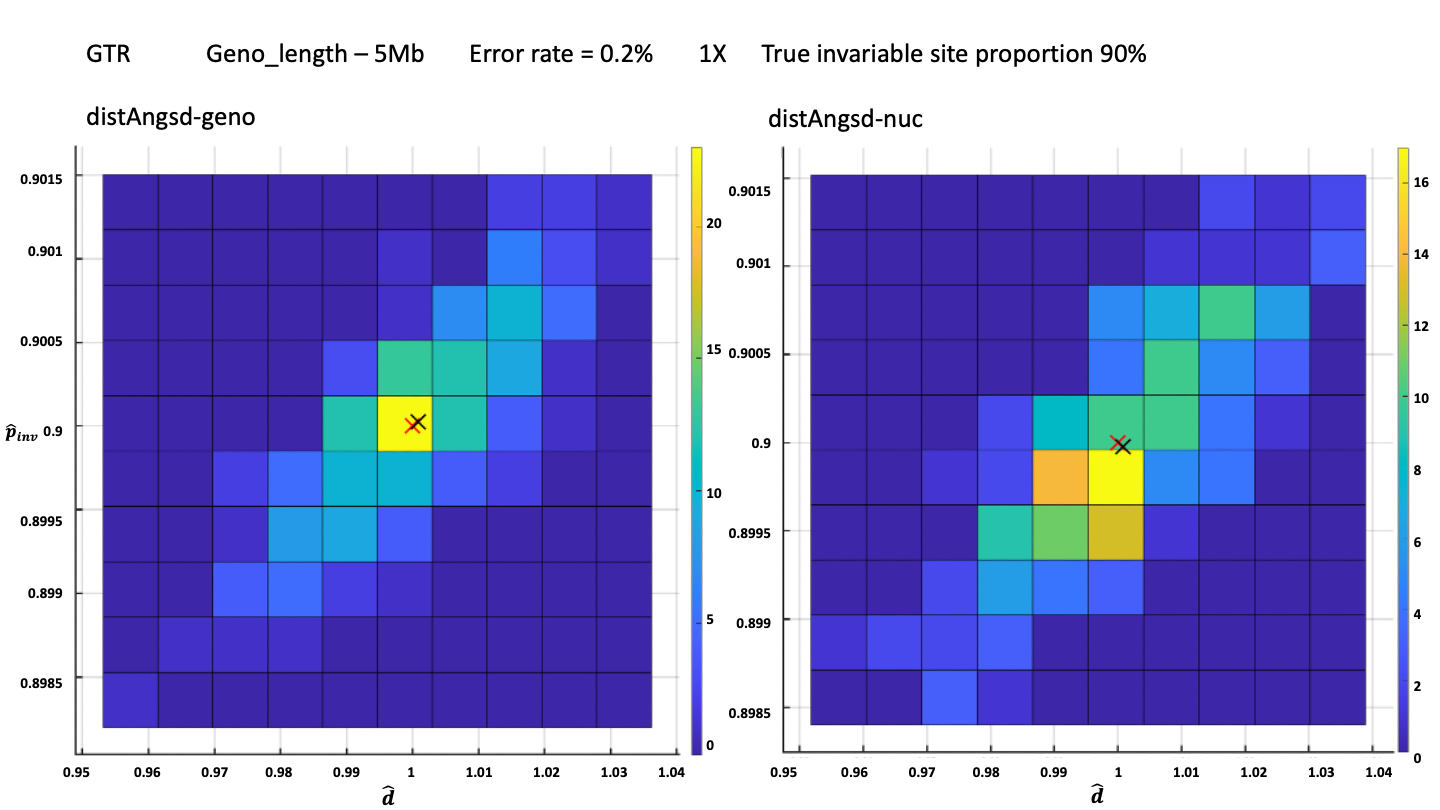
\includegraphics[width=.99\linewidth]{5M90.png}  
  \caption{}
  \label{fig:2D90s1}
\end{subfigure}
\begin{subfigure}{.5\textwidth}
  \centering
  % include second image
  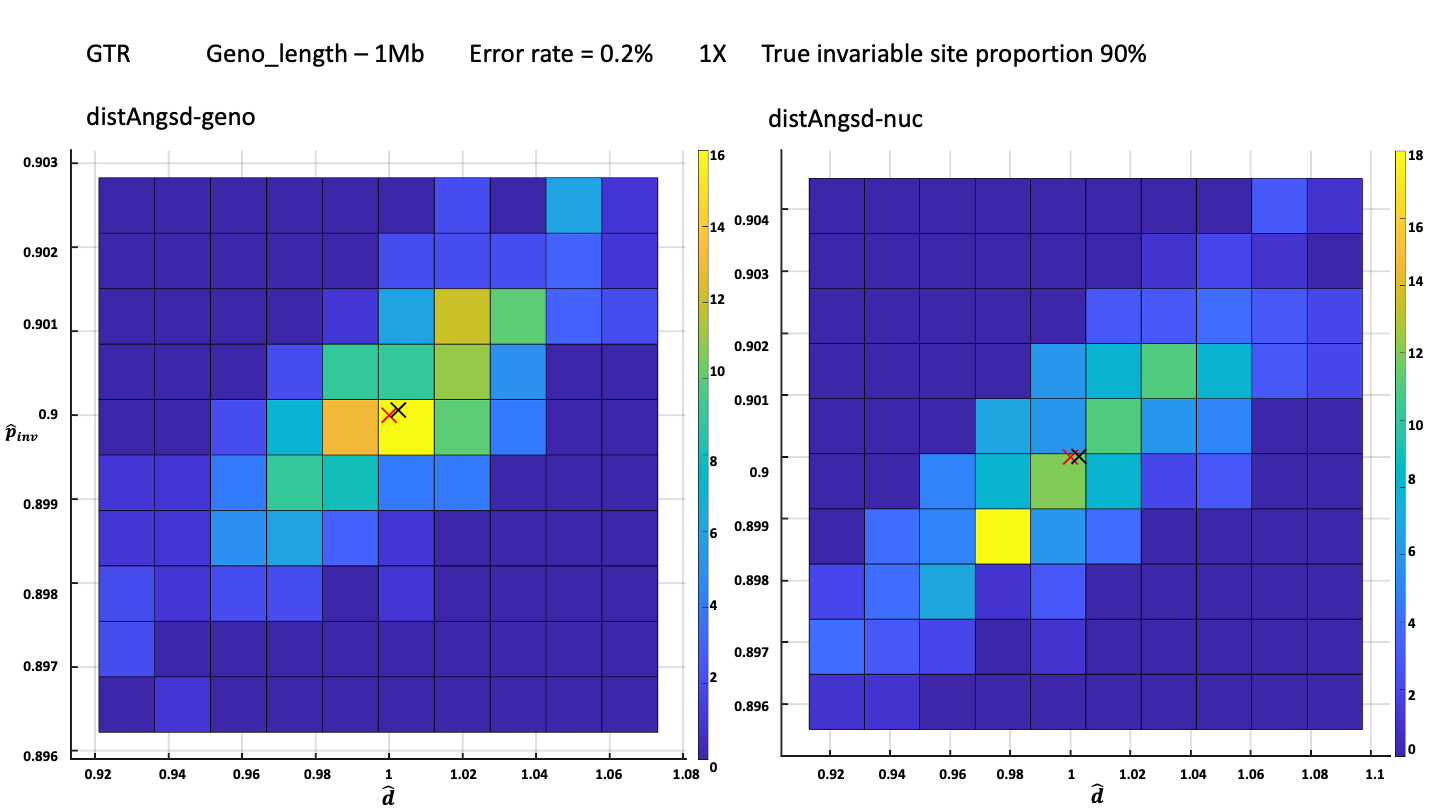
\includegraphics[width=.99\linewidth]{1M90.png}  
  \caption{}
  \label{fig:2D90s2}
\end{subfigure}
\newline
\begin{subfigure}{.5\textwidth}
  \centering
  % include third image
  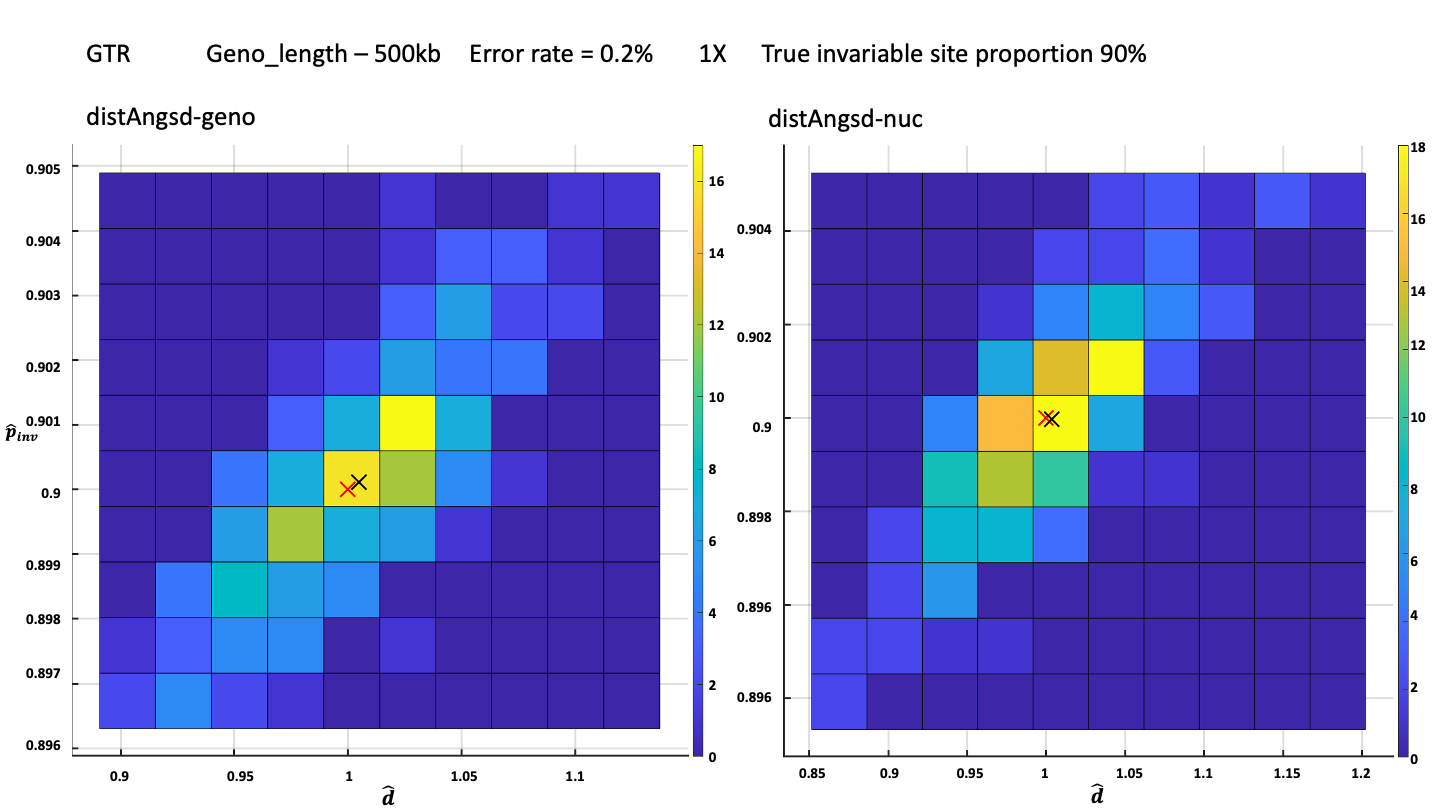
\includegraphics[width=.99\linewidth]{500k90.png}  
  \caption{}
  \label{fig:2D90s3}
\end{subfigure}
\begin{subfigure}{.5\textwidth}
  \centering
  % include fourth image
  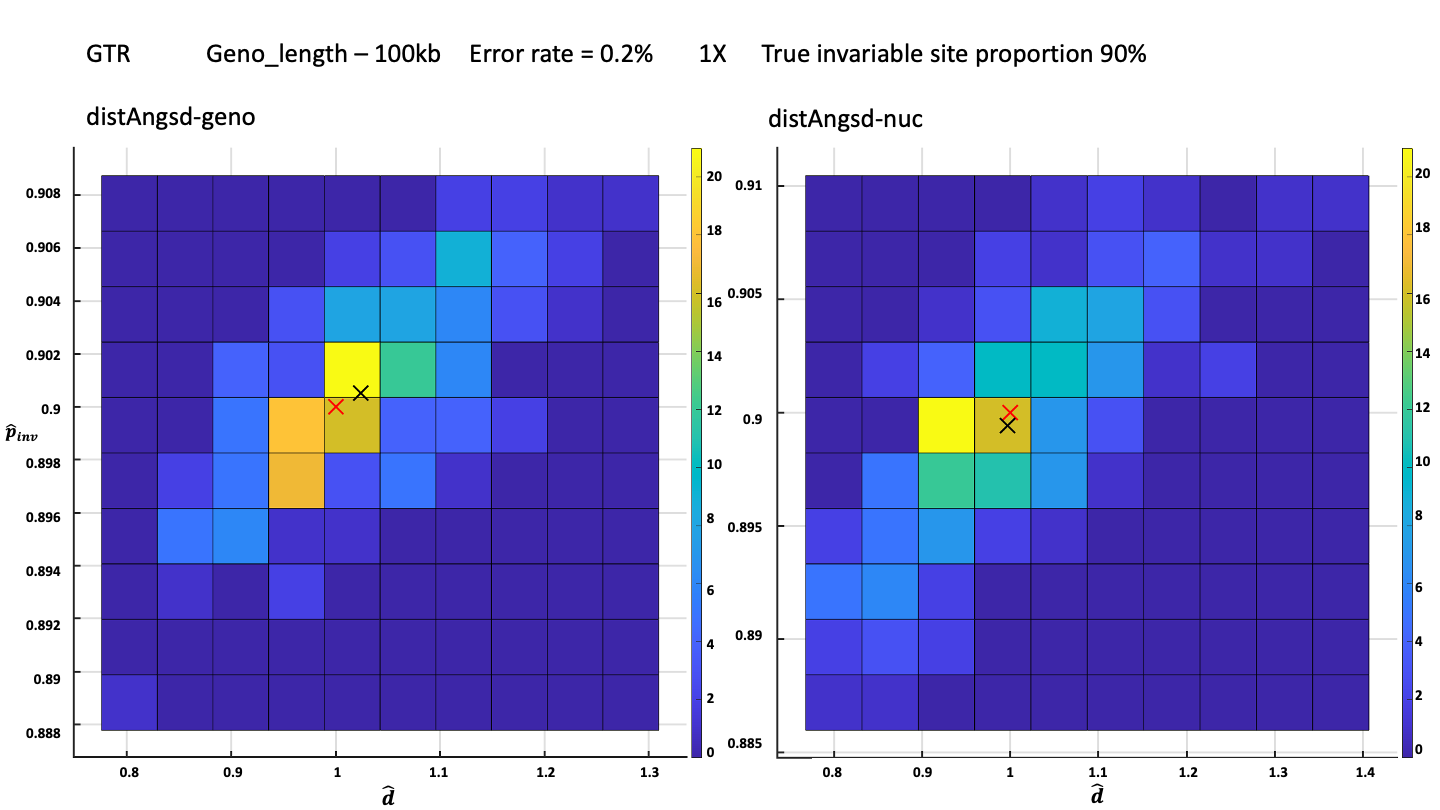
\includegraphics[width=.99\linewidth]{100k90.png}  
  \caption{}
  \label{fig:2D90s4}
\end{subfigure}
\newline
\begin{subfigure}{.5\textwidth}
  \centering
  % include third image
  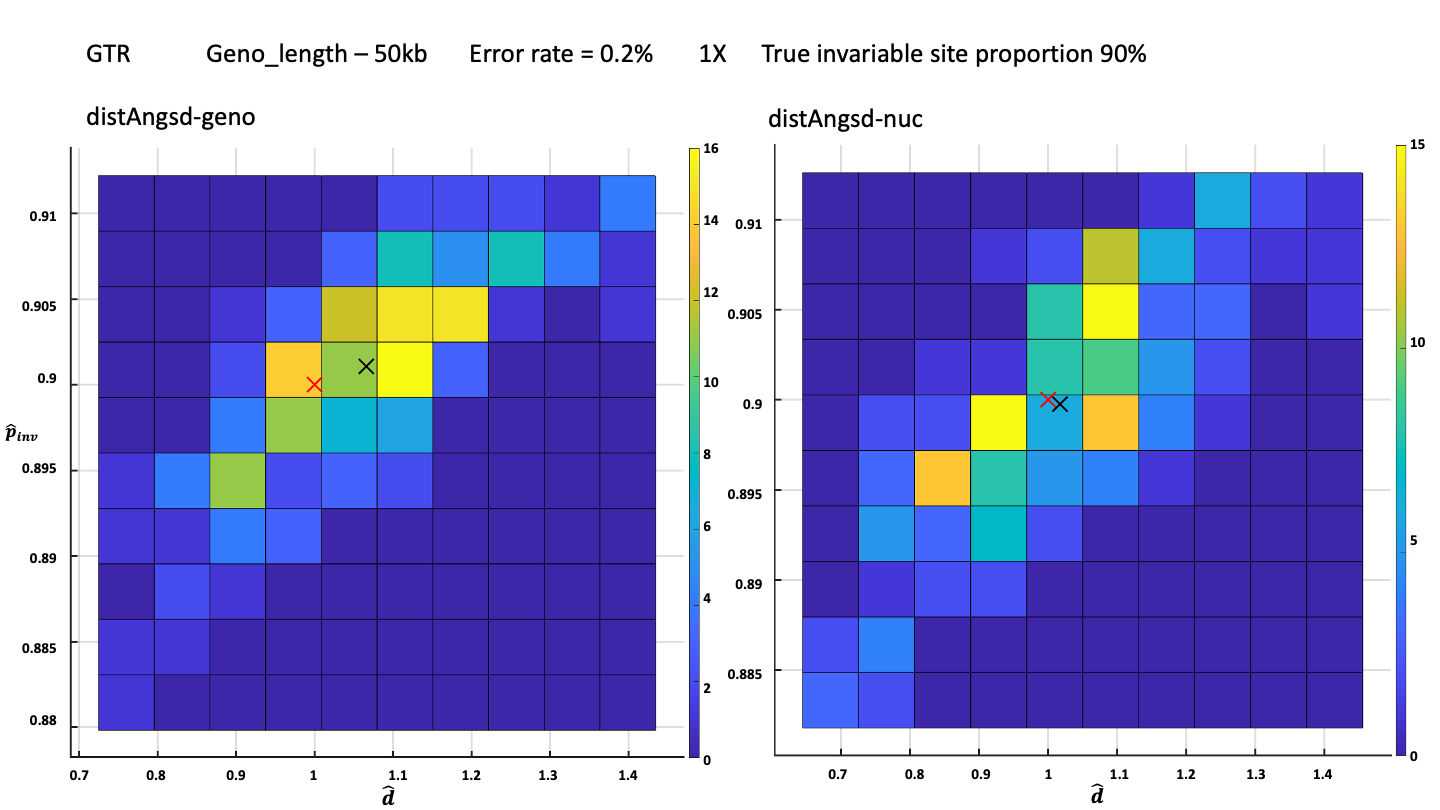
\includegraphics[width=.99\linewidth]{50k90.png}  
  \caption{}
  \label{fig:2D90s5}
\end{subfigure}
\begin{subfigure}{.5\textwidth}
  \centering
  % include fourth image
  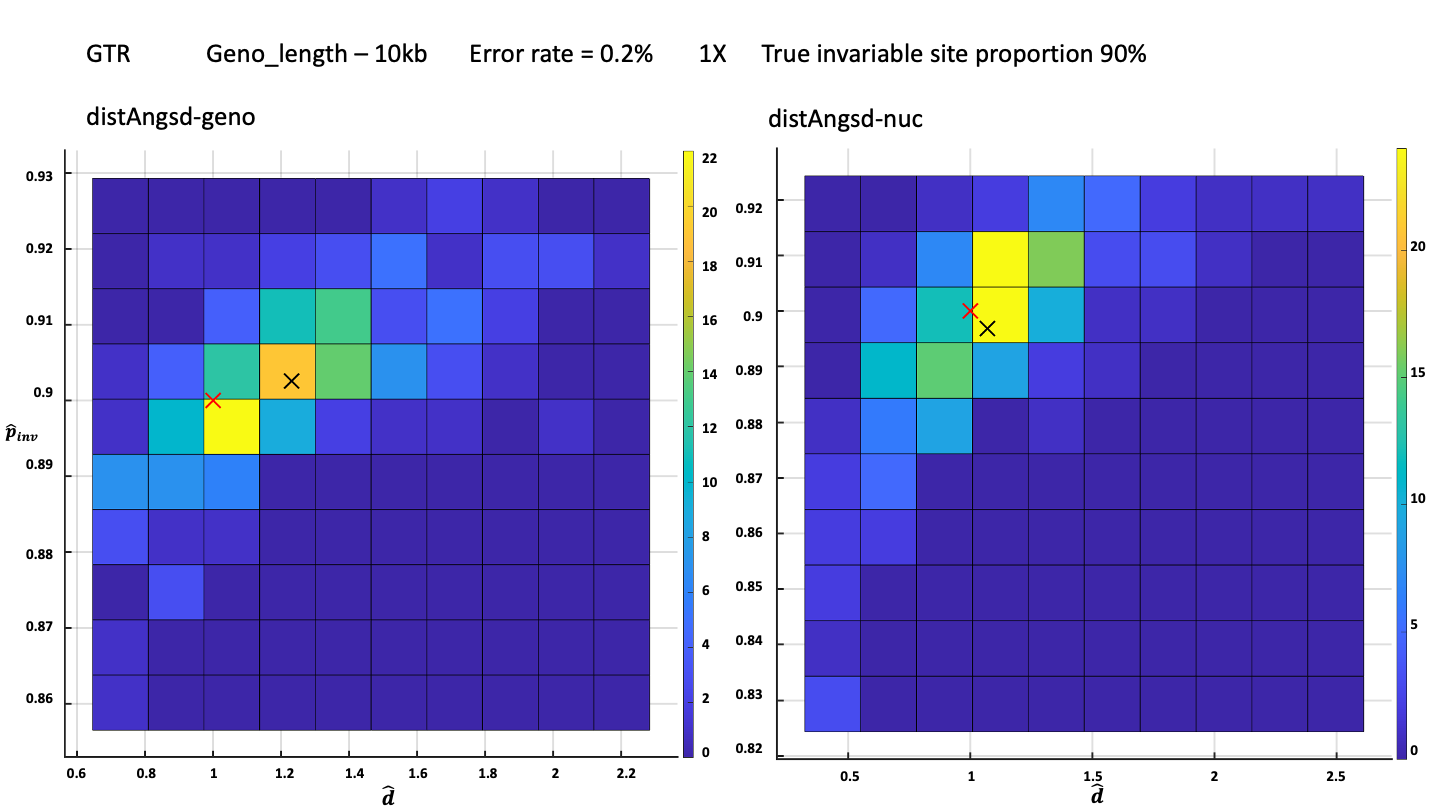
\includegraphics[width=.99\linewidth]{10k90.png}  
  \caption{}
  \label{fig:2D90s6}
\end{subfigure}
\caption{The true fraction of invariable sites is fixed to be $90\%$, and the total genome lengths for inference are varied from $10$Kbp to $5$Mbp, the joint-inference results histogram is present. In all panels, the red cross is the true parameter settings, while the black cross is the inferred mean based on 200 simulated replicates. Simulations follow divergence tree as FIG. 1 in the main text, with $t_1=0.4$ and $t_2 = 0.25$.}
\label{fig:2D90}
\end{figure}



\begin{figure}
\begin{subfigure}{.5\textwidth}
  \centering
  % include first image
  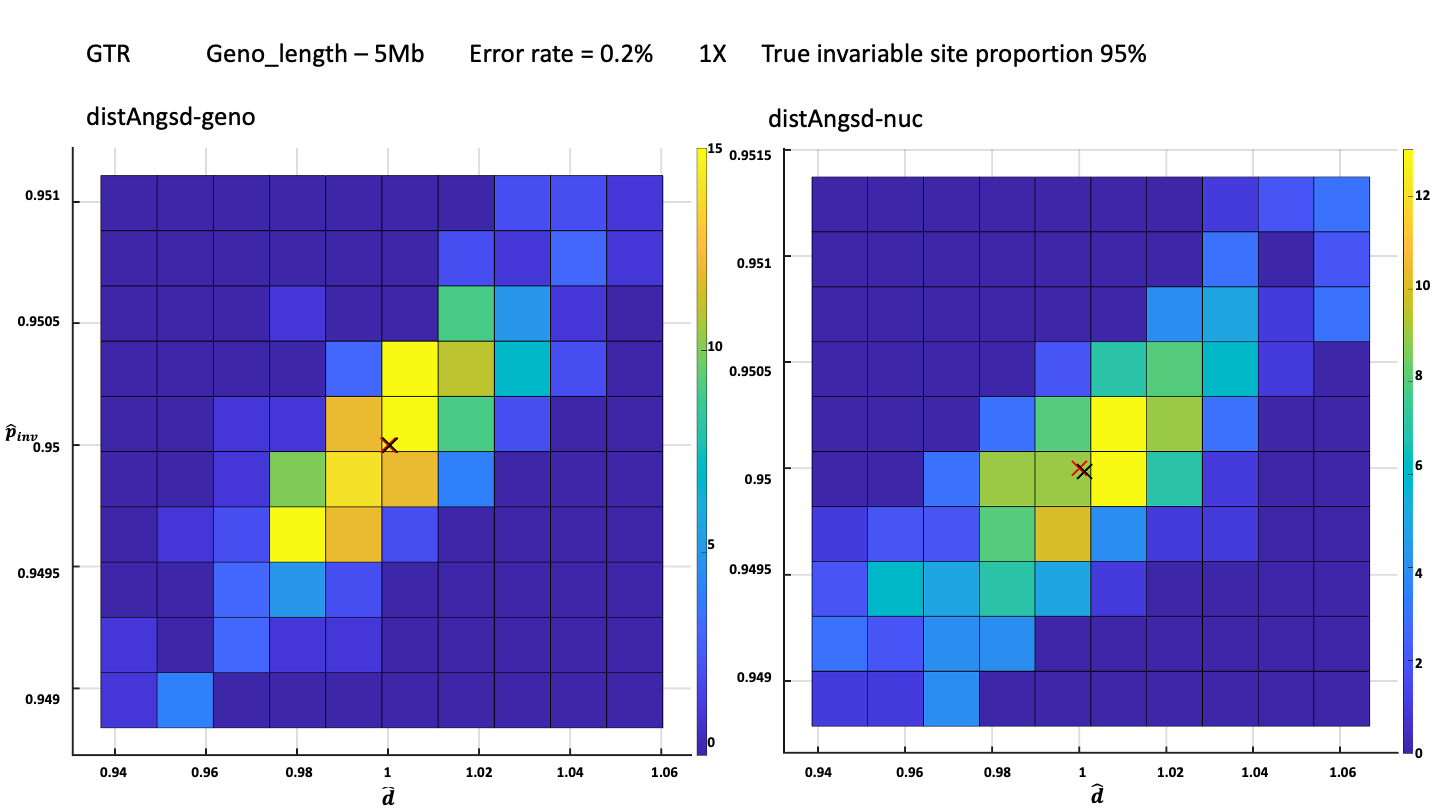
\includegraphics[width=.99\linewidth]{5M95.png}  
  \caption{}
  \label{fig:2D95s1}
\end{subfigure}
\begin{subfigure}{.5\textwidth}
  \centering
  % include second image
  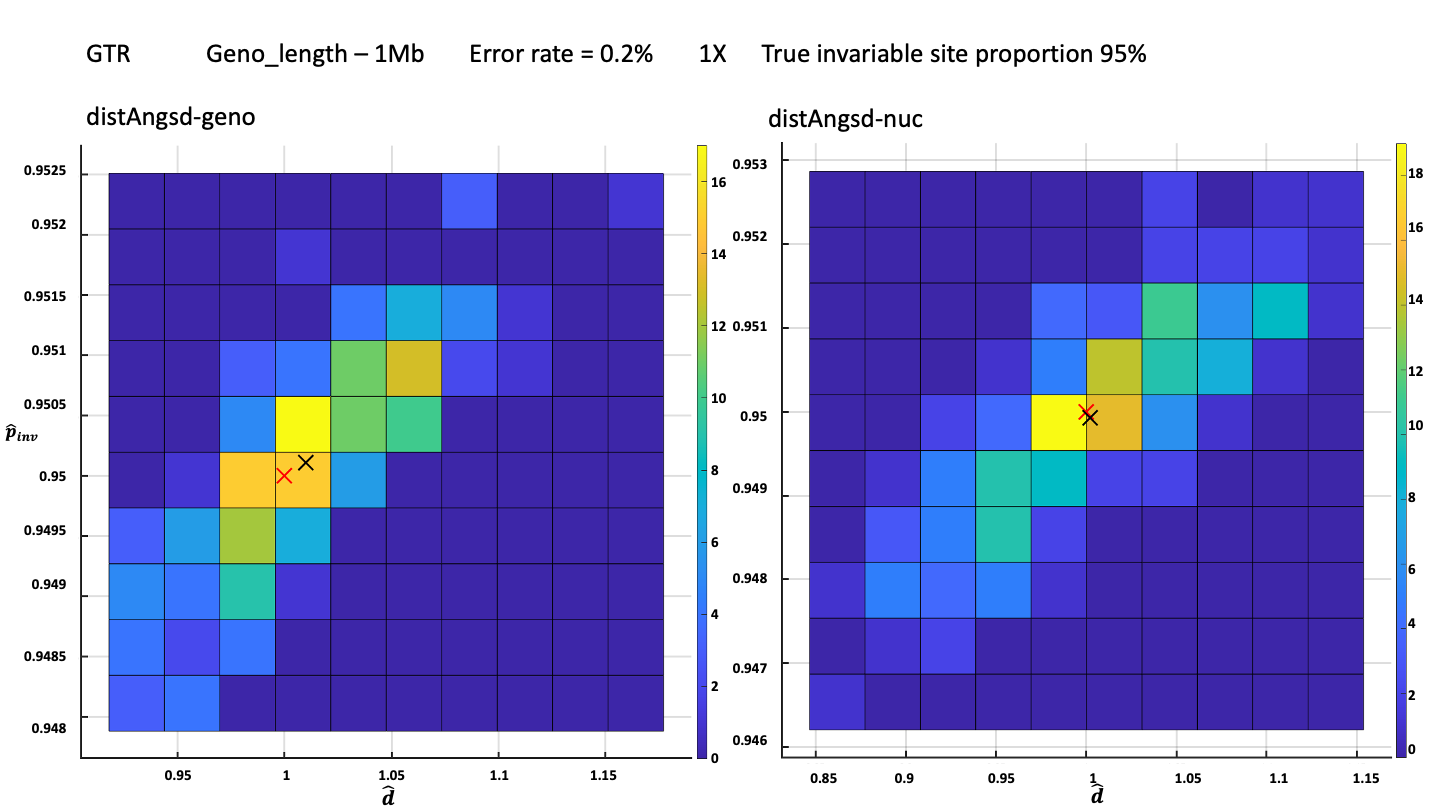
\includegraphics[width=.99\linewidth]{1M95.png}  
  \caption{}
  \label{fig:2D95s2}
\end{subfigure}
\newline
\begin{subfigure}{.5\textwidth}
  \centering
  % include third image
  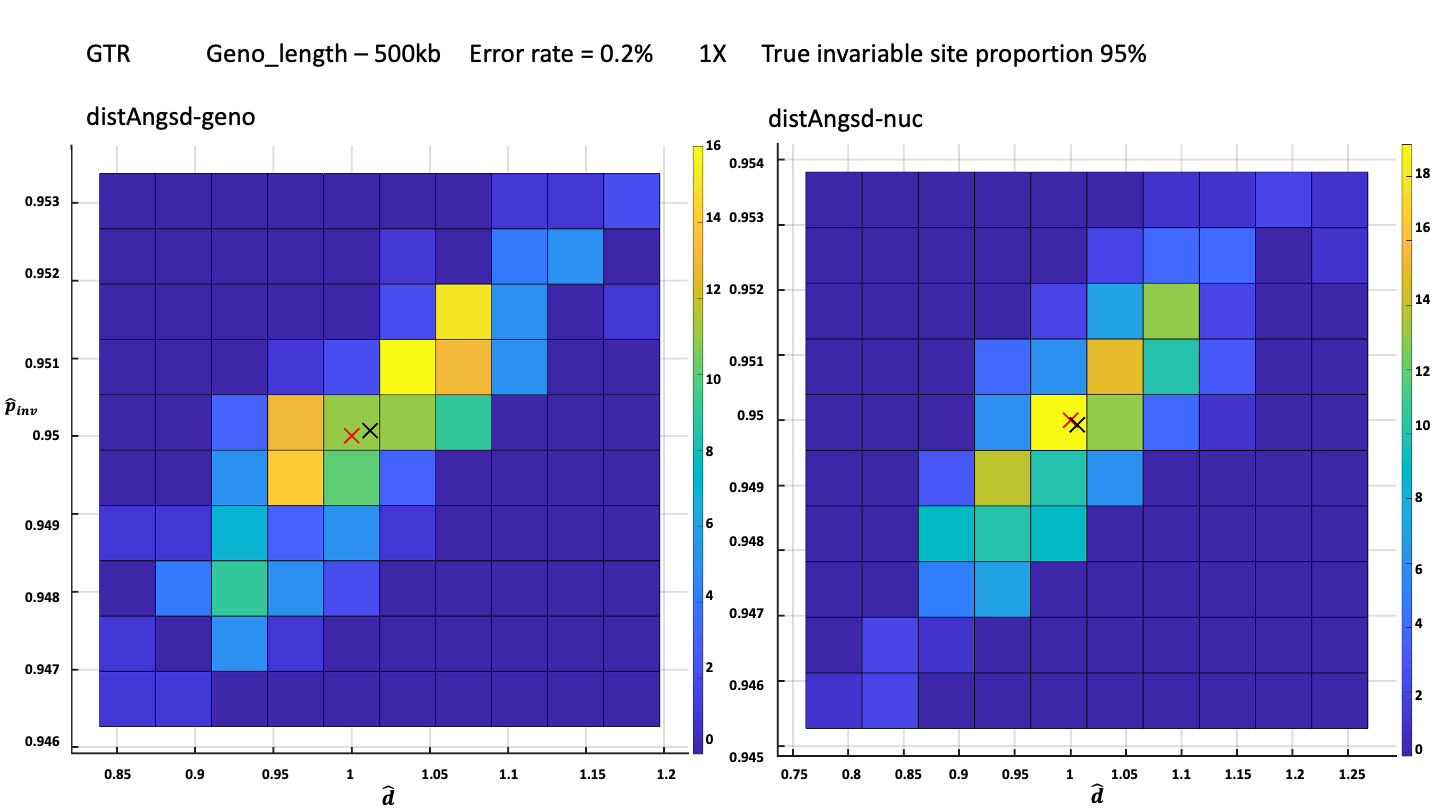
\includegraphics[width=.99\linewidth]{500k95.png}  
  \caption{}
  \label{fig:2D95s3}
\end{subfigure}
\begin{subfigure}{.5\textwidth}
  \centering
  % include fourth image
  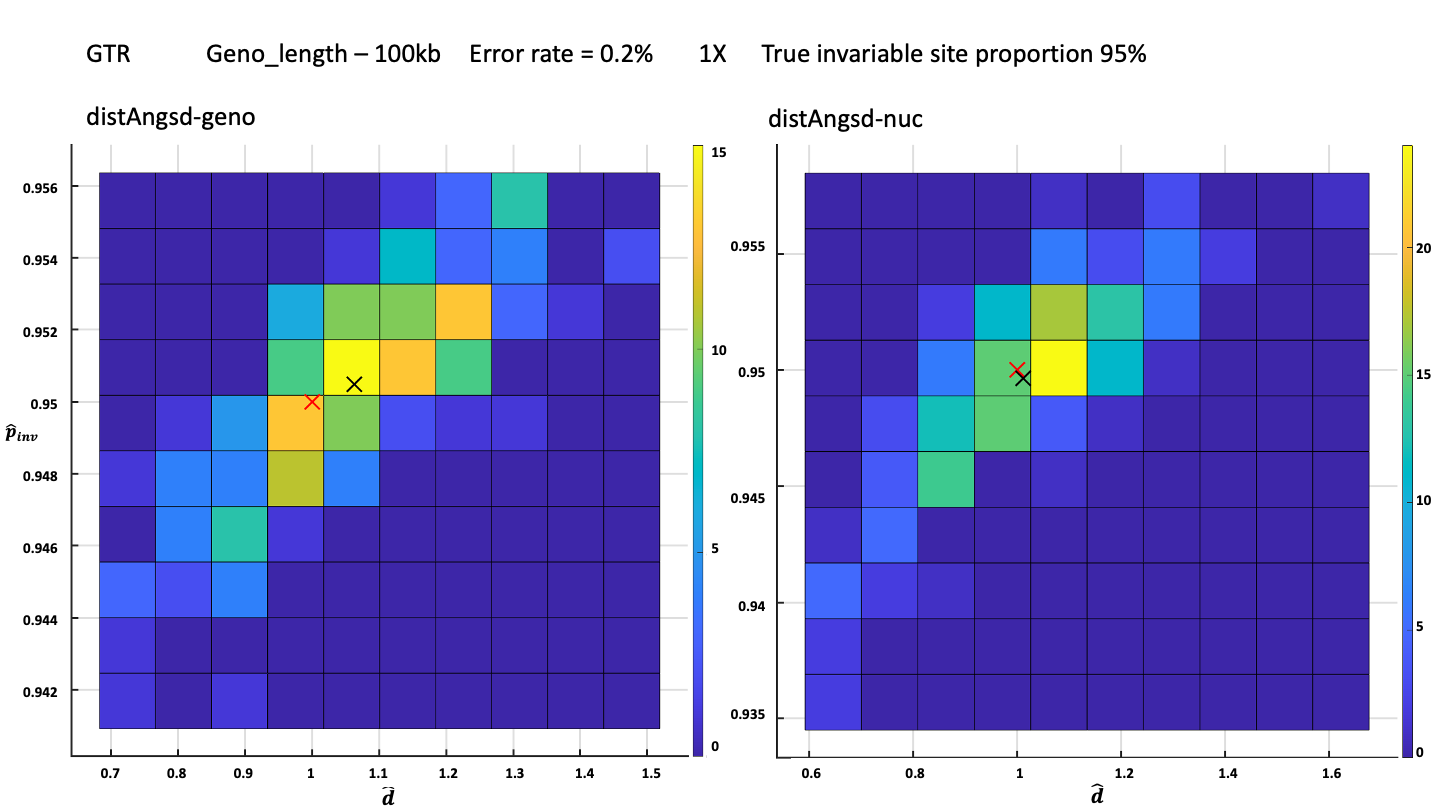
\includegraphics[width=.99\linewidth]{100k95.png}  
  \caption{}
  \label{fig:2D95s4}
\end{subfigure}
\newline
\begin{subfigure}{.5\textwidth}
  \centering
  % include third image
  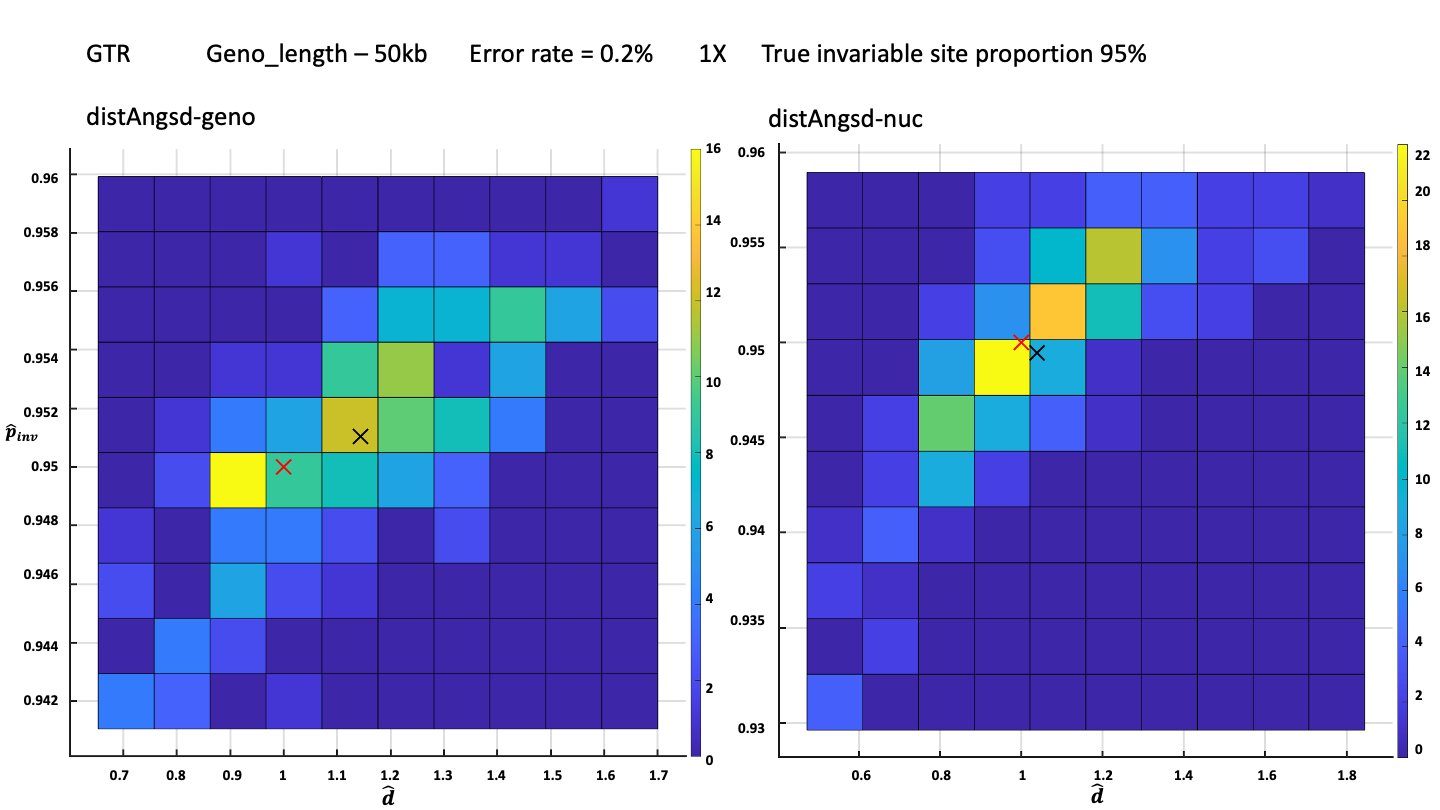
\includegraphics[width=.99\linewidth]{50k95.png}  
  \caption{}
  \label{fig:2D95s5}
\end{subfigure}
\begin{subfigure}{.5\textwidth}
  \centering
  % include fourth image
  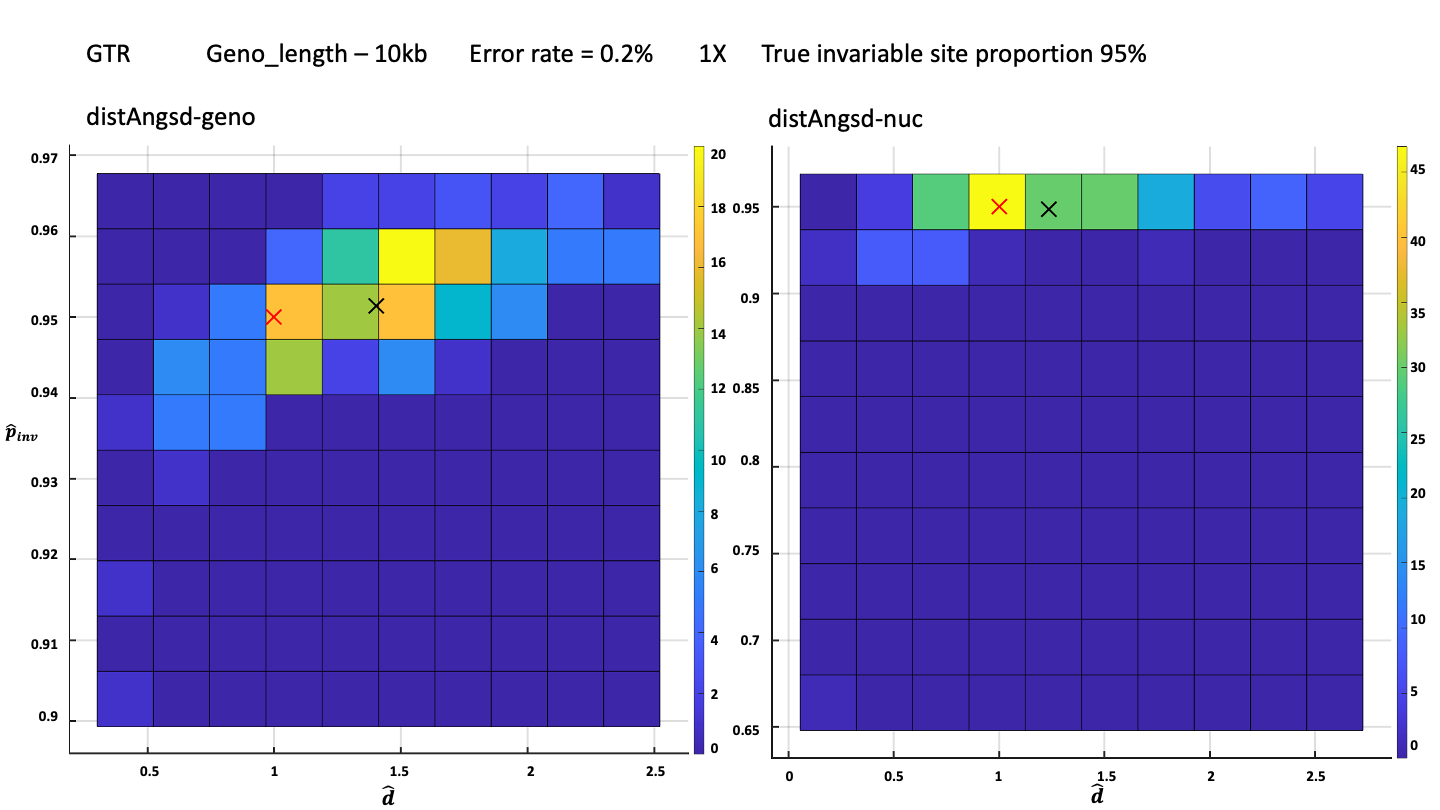
\includegraphics[width=.99\linewidth]{10k95.png}  
  \caption{}
  \label{fig:2D95s6}
\end{subfigure}\caption{The true fraction of invariable sites is fixed to be $95\%$, and the total genome lengths for inference are varied from $10$Kbp to $5$Mbp, the joint-inference results histogram is present. In all panels, the red cross is the true parameter settings, while the black cross is the inferred mean based on 200 simulated replicates. Simulations follow divergence tree as FIG. 1 in the main text, with $t_1=0.4$ and $t_2 = 0.25$.}
\label{fig:2D95}
\end{figure}

\begin{figure}
\begin{subfigure}{.5\textwidth}
  \centering
  % include first image
  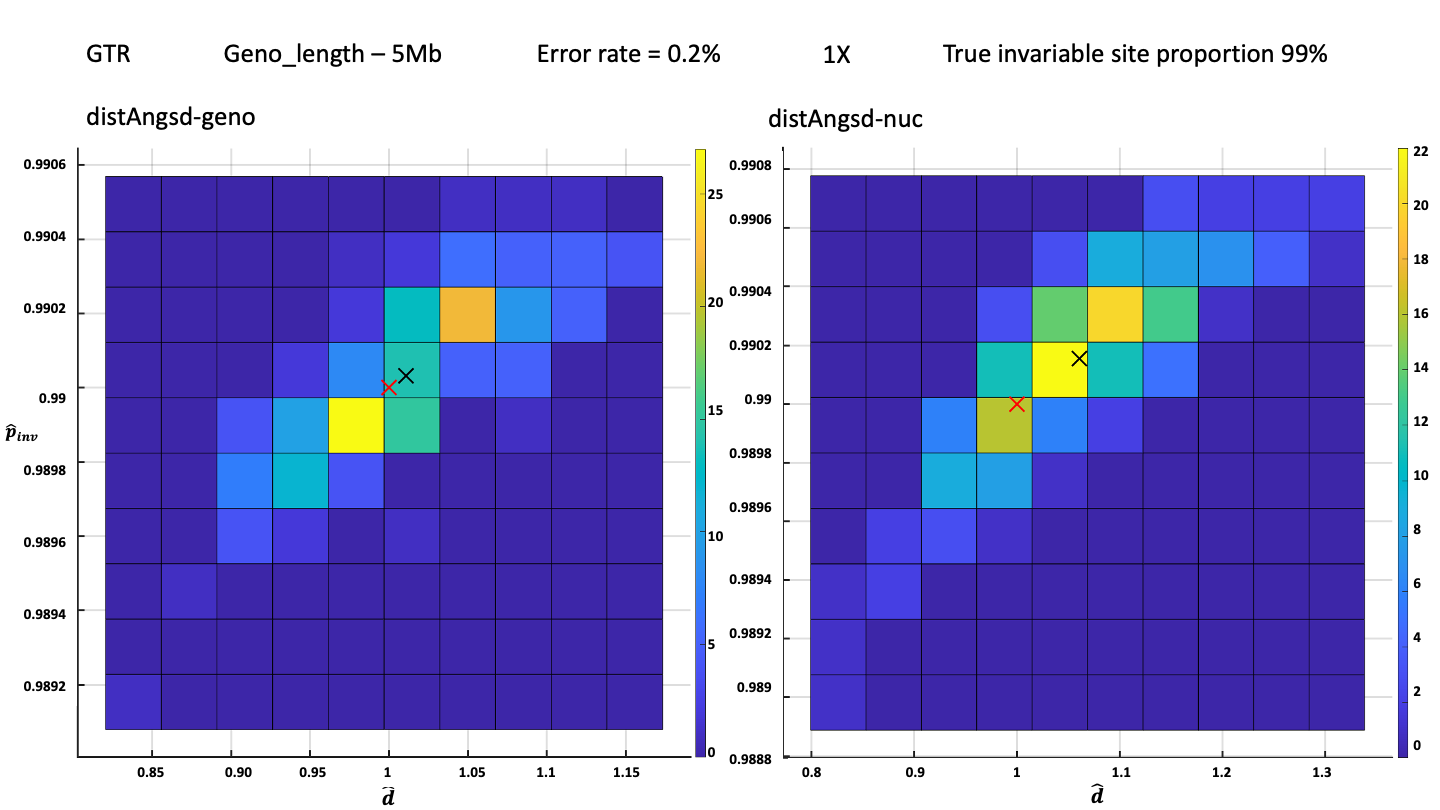
\includegraphics[width=.99\linewidth]{5M99.png}  
  \caption{}
  \label{fig:2D99s1}
\end{subfigure}
\begin{subfigure}{.5\textwidth}
  \centering
  % include second image
  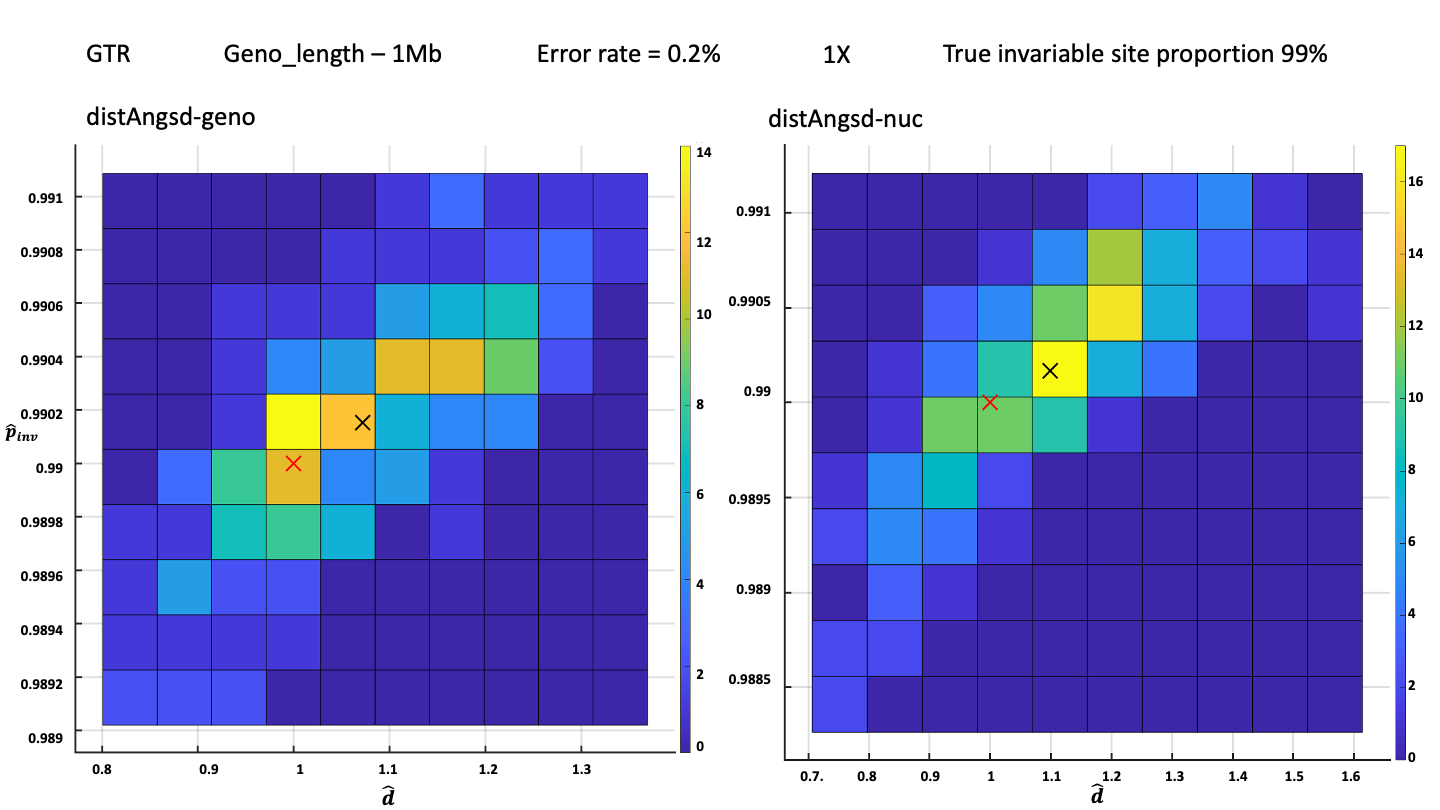
\includegraphics[width=.99\linewidth]{1M99.png}  
  \caption{}
  \label{fig:2D99s2}
\end{subfigure}
\newline
\begin{subfigure}{.5\textwidth}
  \centering
  % include third image
  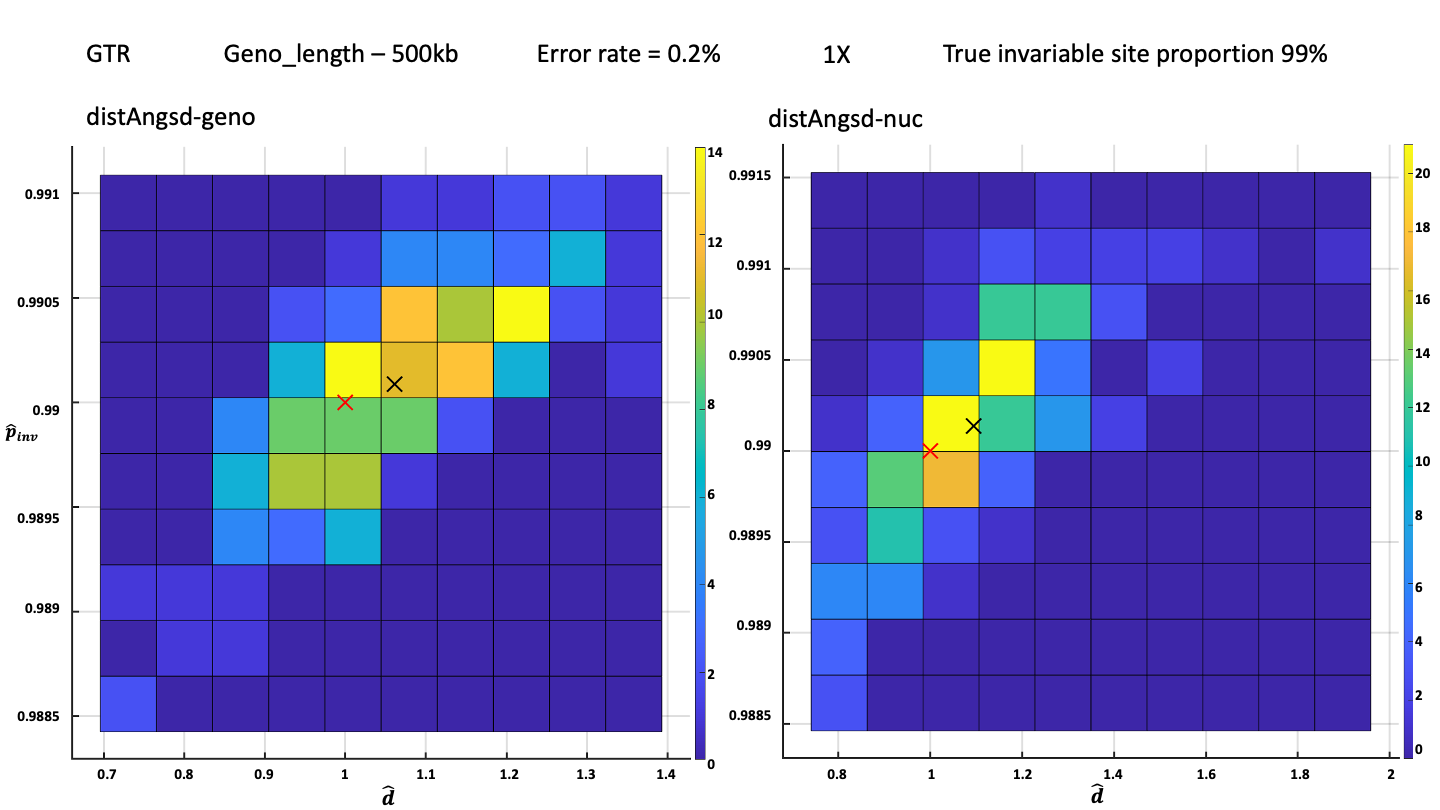
\includegraphics[width=.99\linewidth]{500k99.png}  
  \caption{}
  \label{fig:2D99s3}
\end{subfigure}
\begin{subfigure}{.5\textwidth}
  \centering
  % include fourth image
  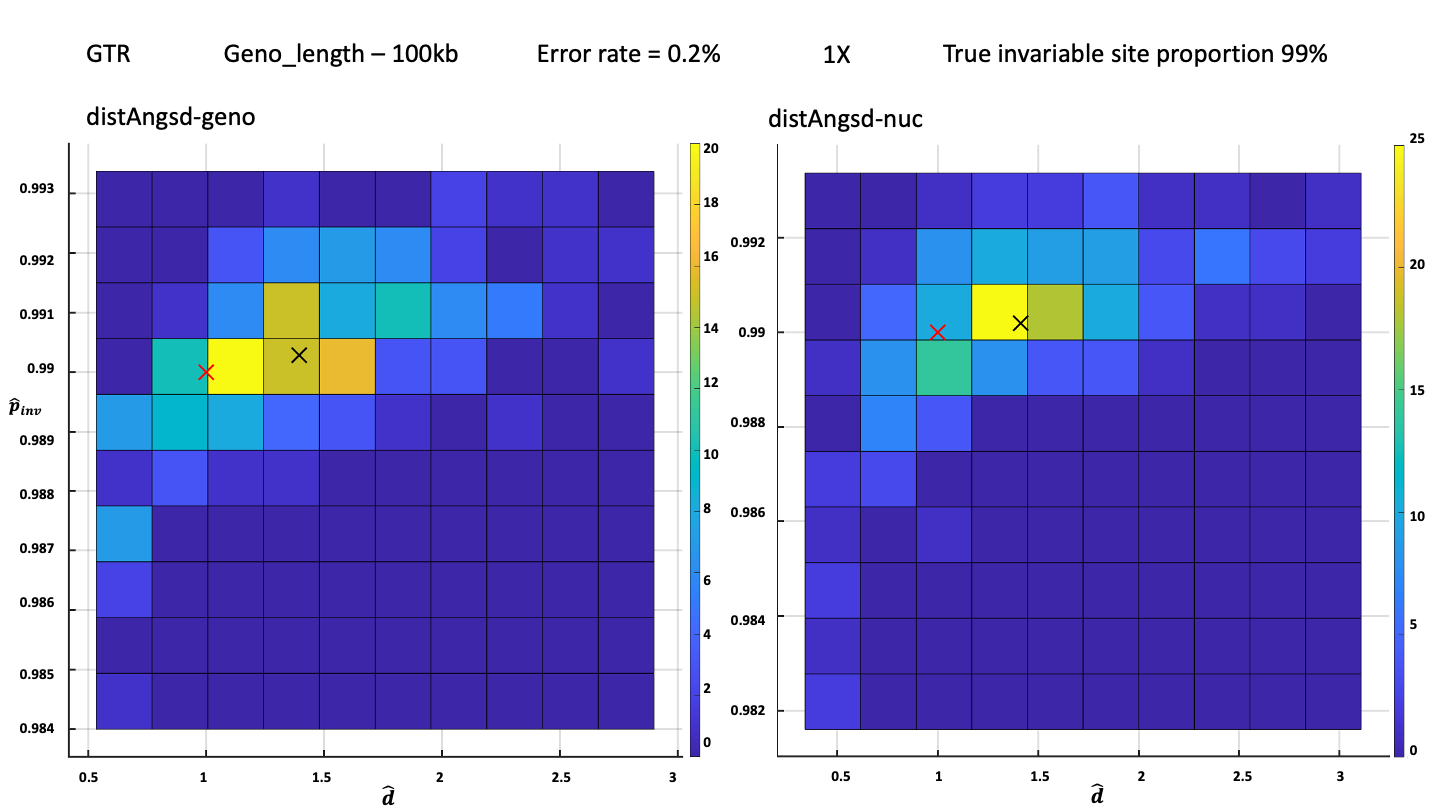
\includegraphics[width=.99\linewidth]{100k99.png}  
  \caption{}
  \label{fig:2D99s4}
\end{subfigure}
\newline
\begin{subfigure}{.5\textwidth}
  \centering
  % include third image
  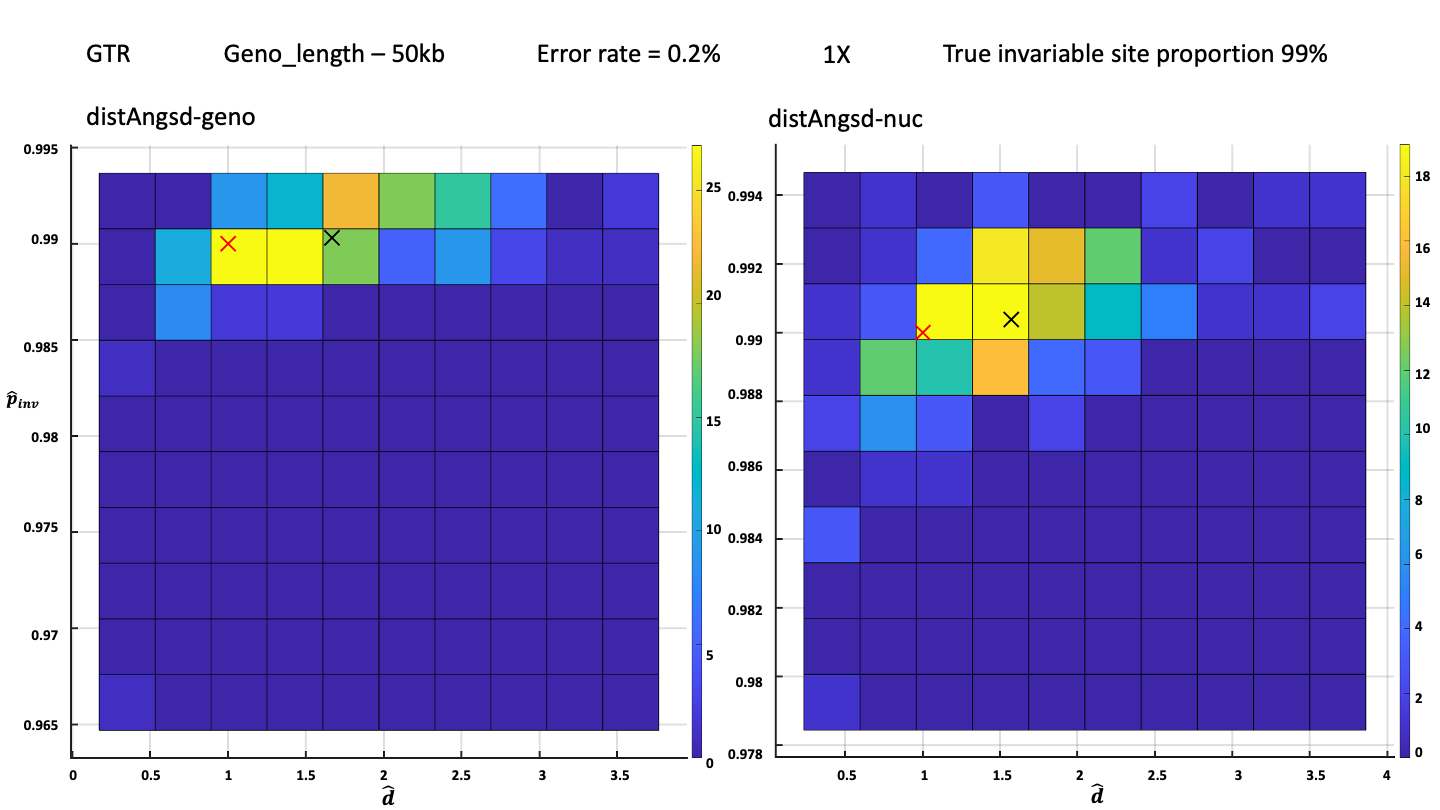
\includegraphics[width=.99\linewidth]{50k99.png}  
  \caption{}
  \label{fig:2D99s5}
\end{subfigure}
\begin{subfigure}{.5\textwidth}
  \centering
  % include fourth image
  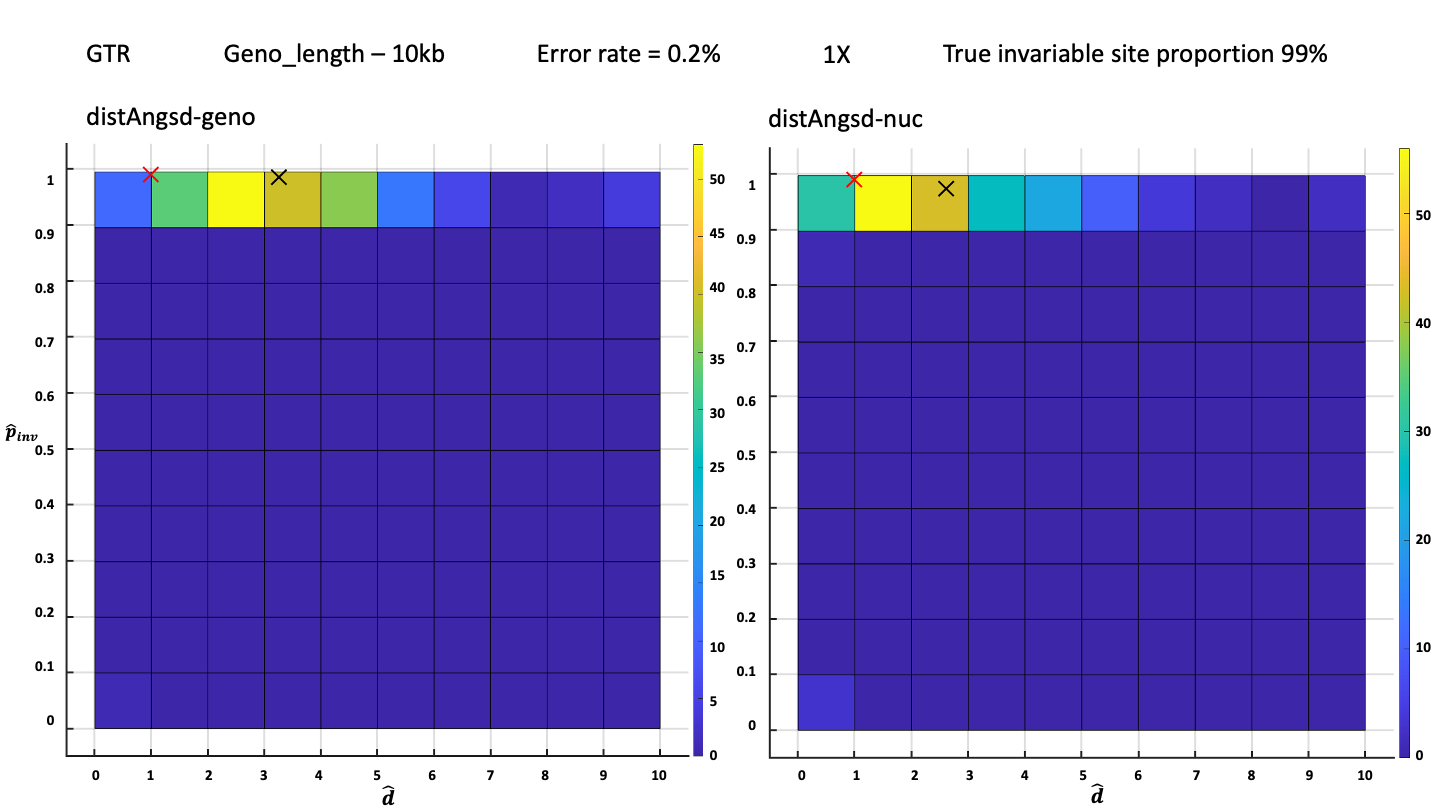
\includegraphics[width=.99\linewidth]{10k99.png}  
  \caption{}
  \label{fig:2D99s6}
\end{subfigure}
\caption{The true fraction of invariable sites is fixed to be $99\%$, and the total genome lengths for inference are varied from $10$Kbp to $5$Mbp, the joint-inference results histogram is present. In all panels, the red cross is the true parameter settings, while the black cross is the inferred mean based on 200 simulated replicates. Simulations follow divergence tree as FIG. 1 in the main text, with $t_1=0.4$ and $t_2 = 0.25$.}
\label{fig:2D99}
\end{figure}

\begin{table}[h]
\centering
 \begin{tabular}{|c|c|c|c|c|c|c|c|c|} 
 \hline
\multirow{2}{*}{Gen. Len.} & \multirow{2}{*}{Method} & \multirow{2}{*}{Par.} &  \multicolumn{2}{c|}{$p_{inv}=90\%$} & \multicolumn{2}{c|}{$p_{inv}=95\%$} & \multicolumn{2}{c|}{$p_{inv}=99\%$} \\ 
\cline{4-9}
&&&Mean&Std&Mean&Std&Mean&Std\\
 \hline
 \multirow{8}{*}{\rotatebox[origin=c]{90}{5Mbp}} & \multirow{2}{*}{distAngsd-geno} & $\hat{d}$ & 1.00084 & 1.35953E-2 & 1.00045 & 2.10988E-2 & 1.01074 & 6.00366E-2\\  
 && $\hat{p}_{inv}$ & 0.900026 & 5.79833E-4 & 0.949999 & 4.25864E-4 & 0.990031 & 2.17424E-4
 \\\cline{2-9}
 &\multirow{2}{*}{distAngsd-nuc} & $\hat{d}$ & 1.00076 & 1.50337E-2 & 1.00124 & 2.70129E-2 & 1.06083 & 9.29861E-2\\
 && $\hat{p}_{inv}$ & 0.899977 & 6.10580E-4 & 0.949986 & 5.22261E-4 & 0.990155 & 3.01781E-4 \\
 \cline{2-9}
 &\multirow{2}{*}{RandomSEQ} & $\hat{d}$ & 1.58853 & 1.55313E-2 & 2.15113 & 2.70029E-2 & 5.44967 & 8.84883E-2\\
 && $\hat{p}_{inv}$ & 0.905106 & 3.81941E-4 & 0.951553 & 2.38171E-4 & 0.986263 & 1.16011E-4\\
 \cline{2-9}
 &\multirow{2}{*}{ConsensusSEQ} & $\hat{d}$ & 1.51601 & 1.50831E-2 & 2.01192 & 2.67129E-2 & 5.03660 & 8.52046E-2\\
 && $\hat{p}_{inv}$ & 0.905014 & 3.65485E-4 & 0.951918 & 2.44095E-4 & 0.986940 & 1.04703E-4\\
 \cline{2-9}
%  &\multirow{2}{*}{ConsensusGT} & $\hat{d}$ & 1.63318 & 1.48248E-2 & 2.23652 & 2.36919E-2 & 5.73002 & 9.02564E-2\\
%  && $\hat{p}_{inv}$ & 0.905102 & 3.24061E-4 & 0.951299 & 2.25359E-4 & 0.985817 & 1.08587E-4\\
 \hline
 \multirow{8}{*}{\rotatebox[origin=c]{90}{1Mbp}} & \multirow{2}{*}{distAngsd-geno} & $\hat{d}$ & 1.00243 & 2.94724E-2 & 1.00979 & 4.39758E-2 & 1.07186 & 1.15771E-1\\ 
 && $\hat{p}_{inv}$ & 0.900061 & 1.17441E-3 & 0.950111 & 8.84607E-4 & 0.990152 & 4.02355E-4
 \\\cline{2-9}
 &\multirow{2}{*}{distAngsd-nuc} & $\hat{d}$ & 1.00277 & 3.94690E-2 & 1.00226 & 5.89451E-2 & 1.09877  & 1.77596E-1\\
 && $\hat{p}_{inv}$ & 0.900007 & 1.64247E-3 & 0.949931 & 1.17688E-3 & 0.990168 & 5.55086E-4 \\
 \cline{2-9}
 &\multirow{2}{*}{RandomSEQ} & $\hat{d}$ & 1.58882 & 3.08462E-2 & 2.15286 & 5.94655E-2 & 5.48705 & 2.0716E-1\\
 && $\hat{p}_{inv}$ & 0.905010 & 8.32686E-4 & 0.951519 & 5.01367E-4 & 0.986264 & 2.37537E-4\\
 \cline{2-9}
 &\multirow{2}{*}{ConsensusSEQ} & $\hat{d}$ & 1.51329 & 3.65318E-2 & 2.01362 & 5.53934E-2 & 5.05441 & 2.17131E-1\\
 && $\hat{p}_{inv}$ & 0.904940 & 3.65485E-4 & 0.951881 & 5.50878E-4 & 0.986944 & 2.58279E-4\\
 \cline{2-9}
%  &\multirow{2}{*}{ConsensusGT} & $\hat{d}$ & 1.63550 & 3.32968E-2 & 2.24065 &  5.64766E-2  & 5.76562 & 1.85243E-1\\
%  && $\hat{p}_{inv}$ & 0.905124 & 7.32258E-4 & 0.951319 & 4.76577E-4 & 0.985868 & 2.29146E-4\\
\hline
 \multirow{8}{*}{\rotatebox[origin=c]{90}{500Kbp}} & \multirow{2}{*}{distAngsd-geno} & $\hat{d}$ & 1.00474 & 4.35305E-2 & 1.01205 & 6.86047E-2 & 1.06148 & 1.2731E-1\\ 
 && $\hat{p}_{inv}$ & 0.900112 & 1.78613E-3 & 0.950068 & 1.35196E-3 & 0.990087 & 4.49511E-4
 \\\cline{2-9}
 &\multirow{2}{*}{distAngsd-nuc} & $\hat{d}$ & 1.00366 & 5.41238E-2 & 1.00598 & 8.03118E-2 & 1.09448 & 1.82087E-1\\
 && $\hat{p}_{inv}$ & 0.899962 & 2.22840E-3 & 0.949934 & 1.57019E-3 & 0.990134 & 5.50317E-4 \\
 \cline{2-9}
 &\multirow{2}{*}{RandomSEQ} & $\hat{d}$ & 1.59016 & 4.85004E-2 & 2.14448 & 7.62341E-2 & 5.47331 & 2.22561E-1\\
 && $\hat{p}_{inv}$ & 0.905139 & 1.28808E-3 & 0.951447 & 7.89837E-4 & 0.986271 & 2.54041E-4\\
 \cline{2-9}
 &\multirow{2}{*}{ConsensusSEQ} & $\hat{d}$ & 1.51674 & 5.11176E-2 & 2.01451 & 8.27945E-2 & 5.04455 & 1.89466E-1\\
 && $\hat{p}_{inv}$ & 0.905021 & 1.18872E-3 & 0.951887 & 7.77788E-4 & 0.986965 & 2.38869E-4\\
 \cline{2-9}
%  &\multirow{2}{*}{ConsensusGT} & $\hat{d}$ & 1.63204 & 4.72295E-2 & 2.22468 & 7.94532E-2 & 5.72468 & 1.83845E-1\\
%  && $\hat{p}_{inv}$ & 0.905027 & 1.07417E-3 & 0.951251 & 6.73326E-4 & 0.985804 & 2.3866E-4\\
 \hline
 \multirow{8}{*}{\rotatebox[origin=c]{90}{100Kbp}} & \multirow{2}{*}{distAngsd-geno} & $\hat{d}$ & 1.02406 & 8.85786E-2 & 1.06314 & 1.54852E-1 & 1.39473 & 4.66236E-1\\ 
 && $\hat{p}_{inv}$ & 0.900518 & 3.3606E-3 & 0.950482 & 2.88867E-3 & 0.990285 & 1.29136E-3
 \\\cline{2-9}
 &\multirow{2}{*}{distAngsd-nuc} & $\hat{d}$ & 0.996977 & 1.08215E-1 & 1.01212 & 1.79275E-1 & 1.41212 & 5.43539E-1\\
 && $\hat{p}_{inv}$ & 0.899429 & 4.6055E-3 & 0.94964 & 3.99864E-3 & 0.990193 & 1.71568E-3 \\
 \cline{2-9}
 &\multirow{2}{*}{RandomSEQ} & $\hat{d}$ & 1.57363 & 1.18014E-1 & 2.15058 & 1.91424E-1 & 5.52584 & 6.41554E-1\\
 && $\hat{p}_{inv}$ & 0.904676 & 2.69941E-3 & 0.951608 & 1.64246E-3 & 0.986317 & 8.05106E-4\\
 \cline{2-9}
 &\multirow{2}{*}{ConsensusSEQ} & $\hat{d}$ & 1.51165 & 1.0918E-1 & 2.00453 & 1.79315E-1 & 5.13561 & 6.79702E-1\\
 && $\hat{p}_{inv}$ & 0.904674 & 3.00162E-3 & 0.95185 & 1.70969E-3 & 0.98695 & 7.27038E-4\\
 \cline{2-9}
%  &\multirow{2}{*}{ConsensusGT} & $\hat{d}$ & 1.64136 & 1.12114E-1 & 2.23646 & 1.90602E-1 & 5.75342 & 6.48596E-1\\
%  && $\hat{p}_{inv}$ & 0.905301 & 2.52405E-3 & 0.951284 & 1.51572E-3 & 0.985789 & 7.55743E-4\\
 \hline
 \multirow{8}{*}{\rotatebox[origin=c]{90}{50Kbp}} & \multirow{2}{*}{distAngsd-geno} & $\hat{d}$ & 1.06608 & 1.37263E-1 & 1.14358 & 2.15256E-1 & 1.6696 & 6.58458E-1\\ 
 && $\hat{p}_{inv}$ & 0.901059 & 5.45958E-3 & 0.951052 & 3.61987E-3 & 0.990282 & 2.37024E-3
 \\\cline{2-9}
 &\multirow{2}{*}{distAngsd-nuc} & $\hat{d}$ & 1.0166 & 1.54537E-1 & 1.03817 & 2.42403E-1 & 1.57237 & 6.32799E-1\\
 && $\hat{p}_{inv}$ & 0.899769 & 6.34495E-3 & 0.949458 & 5.61734E-3 & 0.990396 & 1.93656E-3 \\
 \cline{2-9}
 &\multirow{2}{*}{RandomSEQ} & $\hat{d}$ & 1.59513 & 1.59705E-1 & 2.14888 & 2.74565E-1 & 5.50324 & 1.00235E0\\
 && $\hat{p}_{inv}$ & 0.904825 & 3.43341E-3 & 0.951504 & 2.43478E-3 & 0.986258 & 1.13039E-3\\
 \cline{2-9}
 &\multirow{2}{*}{ConsensusSEQ} & $\hat{d}$ & 1.51946 & 1.56266E-1 & 2.01427 & 2.4944E-1 & 5.12034 & 9.45628E-1\\
 && $\hat{p}_{inv}$ & 0.904801 & 3.58071E-3 & 0.95164 & 2.52908E-3 & 0.986907 & 1.11402E-3\\
%  \cline{2-9}
%  &\multirow{2}{*}{ConsensusGT} & $\hat{d}$ & 1.64366 & 1.51722E-1 & 2.22062 & 2.52137E-1 & 5.82562 & 9.03633E-1\\
%  && $\hat{p}_{inv}$ & 0.90501 & 3.5274E-3 & 0.950976 & 2.3074E-3 & 0.985954 & 9.51243E-4\\
 \hline
  \multirow{8}{*}{\rotatebox[origin=c]{90}{10Kbp}} & \multirow{2}{*}{distAngsd-geno} & $\hat{d}$ & 1.23081 & 3.13099E-1 & 1.40251 & 4.45666E-1 & 3.26442 & 1.77947E0\\  
 && $\hat{p}_{inv}$ & 0.902555 & 1.06004E-2 & 0.951413 & 8.21313E-3 & 0.984776 & 7.0031E-2
 \\\cline{2-9}
 &\multirow{2}{*}{distAngsd-nuc} & $\hat{d}$ & 1.06983 & 3.48114E-1 & 1.23629 & 5.2726E-1 & 2.61881 & 1.73708E0\\
 && $\hat{p}_{inv}$  & 0.896881 & 1.71272E-2 & 0.94875 & 2.39318E-2 & 0.974021 & 1.21019E-1 \\
 \cline{2-9}
 &\multirow{2}{*}{RandomSEQ} & $\hat{d}$ & 1.58182 & 3.59255E-1 & 2.20727 & 5.42745E-1 & 5.75983 & 2.19575E0\\
 && $\hat{p}_{inv}$ & 0.903743 & 8.92097E-3 & 0.951393 & 5.45315E-3 & 0.986127 & 2.41035E-2 \\
 \cline{2-9}
 &\multirow{2}{*}{ConsensusSEQ} & $\hat{d}$ & 1.51719 & 3.55823E-1 & 2.07518 & 6.31764E-1 & 5.3562 & 2.12265E0\\
 && $\hat{p}_{inv}$ & 0.903096 & 9.83004E-3 & 0.95175 & 5.40778E-3 & 0.986886 & 2.68888E-3\\
%  \cline{2-9}
%  &\multirow{2}{*}{ConsensusGT} & $\hat{d}$ & 1.63717 & 3.34337E-1 & 2.3231 & 5.56693E-1 & 5.93941 & 1.95719E0\\
%  && $\hat{p}_{inv}$ & 0.905032 & 8.77189E-3 & 0.951142 & 5.43137E-3 & 0.985605 & 2.16274E-3\\
 \hline
\end{tabular}
\caption{Summary statistics of inferred genetic distance $\hat{d}$ and the fraction of invariable sites $\hat{p}_{inv}$ based on $200$ replicate simulations with different genome lengths and methods. The values are present with $6$ significant figures. Simulations follow divergence tree as FIG. 1 in the main text, with $t_1=0.4$ and $t_2 = 0.25$.}
\label{tab:2DComparisons}
\end{table}
% \begin{table}[ht]
% \centering
%  \begin{tabular}{|c|c|c|c|c|c|c|c|c|} 
%  \hline
% \multirow{2}{*}{Gen. Len.} & \multirow{2}{*}{Method} & \multirow{2}{*}{Par.} &  \multicolumn{2}{c|}{$p_{inv}=90\%$} & \multicolumn{2}{c|}{$p_{inv}=95\%$} & \multicolumn{2}{c|}{$p_{inv}=99\%$} \\ 
% \cline{4-9}
% &&&Mean&Std&Mean&Std&Mean&Std\\
%  \hline
%  \multirow{10}{*}{\rotatebox[origin=c]{90}{5Mbp}} & \multirow{2}{*}{distAngsd-geno} & $\hat{d}$ & 1.00084 & 1.35953E-2 & 1.00045 & 2.10988E-2 & 1.01074 & 6.00366E-2\\  
%  && $\hat{p}_{inv}$ & 0.900026 & 5.79833E-4 & 0.949999 & 4.25864E-4 & 0.990031 & 2.17424E-4
%  \\\cline{2-9}
%  &\multirow{2}{*}{distAngsd-nuc} & $\hat{d}$ & 1.00076 & 1.50337E-2 & 1.00124 & 2.70129E-2 & 1.06083 & 9.29861E-2\\
%  && $\hat{p}_{inv}$ & 0.899977 & 6.10580E-4 & 0.949986 & 5.22261E-4 & 0.990155 & 3.01781E-4 \\
%  \cline{2-9}
%  &\multirow{2}{*}{RandomSEQ} & $\hat{d}$ & 1.58853 & 1.55313E-2 & 2.15113 & 2.70029E-2 & 5.44967 & 8.84883E-2\\
%  && $\hat{p}_{inv}$ & 0.905106 & 3.81941E-4 & 0.951553 & 2.38171E-4 & 0.986263 & 1.16011E-4\\
%  \cline{2-9}
%  &\multirow{2}{*}{ConsensusSEQ} & $\hat{d}$ & 1.51601 & 1.50831E-2 & 2.01192 & 2.67129E-2 & 5.03660 & 8.52046E-2\\
%  && $\hat{p}_{inv}$ & 0.905014 & 3.65485E-4 & 0.951918 & 2.44095E-4 & 0.986940 & 1.04703E-4\\
%  \cline{2-9}
%  &\multirow{2}{*}{ConsensusGT} & $\hat{d}$ & 1.63318 & 1.48248E-2 & 2.23652 & 2.36919E-2 & 5.73002 & 9.02564E-2\\
%  && $\hat{p}_{inv}$ & 0.905102 & 3.24061E-4 & 0.951299 & 2.25359E-4 & 0.985817 & 1.08587E-4\\
%  \hline
%  \multirow{10}{*}{\rotatebox[origin=c]{90}{1Mbp}} & \multirow{2}{*}{distAngsd-geno} & $\hat{d}$ & 1.00243 & 2.94724E-2 & 1.00979 & 4.39758E-2 & 1.07186 & 1.15771E-1\\ 
%  && $\hat{p}_{inv}$ & 0.900061 & 1.17441E-3 & 0.950111 & 8.84607E-4 & 0.990152 & 4.02355E-4
%  \\\cline{2-9}
%  &\multirow{2}{*}{distAngsd-nuc} & $\hat{d}$ & 1.00277 & 3.94690E-2 & 1.00226 & 5.89451E-2 & 1.09877  & 1.77596E-1\\
%  && $\hat{p}_{inv}$ & 0.900007 & 1.64247E-3 & 0.949931 & 1.17688E-3 & 0.990168 & 5.55086E-4 \\
%  \cline{2-9}
%  &\multirow{2}{*}{RandomSEQ} & $\hat{d}$ & 1.58882 & 3.08462E-2 & 2.15286 & 5.94655E-2 & 5.48705 & 2.0716E-1\\
%  && $\hat{p}_{inv}$ & 0.905010 & 8.32686E-4 & 0.951519 & 5.01367E-4 & 0.986264 & 2.37537E-4\\
%  \cline{2-9}
%  &\multirow{2}{*}{ConsensusSEQ} & $\hat{d}$ & 1.51329 & 3.65318E-2 & 2.01362 & 5.53934E-2 & 5.05441 & 2.17131E-1\\
%  && $\hat{p}_{inv}$ & 0.904940 & 3.65485E-4 & 0.951881 & 5.50878E-4 & 0.986944 & 2.58279E-4\\
%  \cline{2-9}
%  &\multirow{2}{*}{ConsensusGT} & $\hat{d}$ & 1.63550 & 3.32968E-2 & 2.24065 &  5.64766E-2  & 5.76562 & 1.85243E-1\\
%  && $\hat{p}_{inv}$ & 0.905124 & 7.32258E-4 & 0.951319 & 4.76577E-4 & 0.985868 & 2.29146E-4\\
% \hline
%  \multirow{10}{*}{\rotatebox[origin=c]{90}{500Kbp}} & \multirow{2}{*}{distAngsd-geno} & $\hat{d}$ & 1.00474 & 4.35305E-2 & 1.01205 & 6.86047E-2 & 1.06148 & 1.2731E-1\\ 
%  && $\hat{p}_{inv}$ & 0.900112 & 1.78613E-3 & 0.950068 & 1.35196E-3 & 0.990087 & 4.49511E-4
%  \\\cline{2-9}
%  &\multirow{2}{*}{distAngsd-nuc} & $\hat{d}$ & 1.00366 & 5.41238E-2 & 1.00598 & 8.03118E-2 & 1.09448 & 1.82087E-1\\
%  && $\hat{p}_{inv}$ & 0.899962 & 2.22840E-3 & 0.949934 & 1.57019E-3 & 0.990134 & 5.50317E-4 \\
%  \cline{2-9}
%  &\multirow{2}{*}{RandomSEQ} & $\hat{d}$ & 1.59016 & 4.85004E-2 & 2.14448 & 7.62341E-2 & 5.47331 & 2.22561E-1\\
%  && $\hat{p}_{inv}$ & 0.905139 & 1.28808E-3 & 0.951447 & 7.89837E-4 & 0.986271 & 2.54041E-4\\
%  \cline{2-9}
%  &\multirow{2}{*}{ConsensusSEQ} & $\hat{d}$ & 1.51674 & 5.11176E-2 & 2.01451 & 8.27945E-2 & 5.04455 & 1.89466E-1\\
%  && $\hat{p}_{inv}$ & 0.905021 & 1.18872E-3 & 0.951887 & 7.77788E-4 & 0.986965 & 2.38869E-4\\
%  \cline{2-9}
%  &\multirow{2}{*}{ConsensusGT} & $\hat{d}$ & 1.63204 & 4.72295E-2 & 2.22468 & 7.94532E-2 & 5.72468 & 1.83845E-1\\
%  && $\hat{p}_{inv}$ & 0.905027 & 1.07417E-3 & 0.951251 & 6.73326E-4 & 0.985804 & 2.3866E-4\\
%  \hline
%  \multirow{10}{*}{\rotatebox[origin=c]{90}{100Kbp}} & \multirow{2}{*}{distAngsd-geno} & $\hat{d}$ & 1.02406 & 8.85786E-2 & 1.06314 & 1.54852E-1 & 1.39473 & 4.66236E-1\\ 
%  && $\hat{p}_{inv}$ & 0.900518 & 3.3606E-3 & 0.950482 & 2.88867E-3 & 0.990285 & 1.29136E-3
%  \\\cline{2-9}
%  &\multirow{2}{*}{distAngsd-nuc} & $\hat{d}$ & 0.996977 & 1.08215E-1 & 1.01212 & 1.79275E-1 & 1.41212 & 5.43539E-1\\
%  && $\hat{p}_{inv}$ & 0.899429 & 4.6055E-3 & 0.94964 & 3.99864E-3 & 0.990193 & 1.71568E-3 \\
%  \cline{2-9}
%  &\multirow{2}{*}{RandomSEQ} & $\hat{d}$ & 1.57363 & 1.18014E-1 & 2.15058 & 1.91424E-1 & 5.52584 & 6.41554E-1\\
%  && $\hat{p}_{inv}$ & 0.904676 & 2.69941E-3 & 0.951608 & 1.64246E-3 & 0.986317 & 8.05106E-4\\
%  \cline{2-9}
%  &\multirow{2}{*}{ConsensusSEQ} & $\hat{d}$ & 1.51165 & 1.0918E-1 & 2.00453 & 1.79315E-1 & 5.13561 & 6.79702E-1\\
%  && $\hat{p}_{inv}$ & 0.904674 & 3.00162E-3 & 0.95185 & 1.70969E-3 & 0.98695 & 7.27038E-4\\
%  \cline{2-9}
%  &\multirow{2}{*}{ConsensusGT} & $\hat{d}$ & 1.64136 & 1.12114E-1 & 2.23646 & 1.90602E-1 & 5.75342 & 6.48596E-1\\
%  && $\hat{p}_{inv}$ & 0.905301 & 2.52405E-3 & 0.951284 & 1.51572E-3 & 0.985789 & 7.55743E-4\\
%  \hline
% \end{tabular}
% \caption{Summary statistics of inferred genetic distance $\hat{d}$ and the fraction of invariable sites $\hat{p}_{inv}$} based on $200$ replicate simulations with different genome lengths and methods. The values are present with $6$ significant figures. Simulations follow divergence tree as FIG. 1 in the main text, with $t_1=0.4$ and $t_2 = 0.25$.
% \label{tab:2DComparisons}
% \end{table}


% \begin{table}[ht]
% \centering
%  \begin{tabular}{|c|c|c|c|c|c|c|c|c|} 
%  \hline
% \multirow{2}{*}{Gen. Len.} & \multirow{2}{*}{Method} & \multirow{2}{*}{Par.} &  \multicolumn{2}{c|}{$p_{inv}=90\%$} & \multicolumn{2}{c|}{$p_{inv}=95\%$} & \multicolumn{2}{c|}{$p_{inv}=99\%$} \\ 
% \cline{4-9}
% &&&Mean&Std&Mean&Std&Mean&Std\\
%  \hline
%  \multirow{10}{*}{\rotatebox[origin=c]{90}{50Kbp}} & \multirow{2}{*}{distAngsd-geno} & $\hat{d}$ & 1.06608 & 1.37263E-1 & 1.14358 & 2.15256E-1 & 1.6696 & 6.58458E-1\\ 
%  && $\hat{p}_{inv}$ & 0.901059 & 5.45958E-3 & 0.951052 & 3.61987E-3 & 0.990282 & 2.37024E-3
%  \\\cline{2-9}
%  &\multirow{2}{*}{distAngsd-nuc} & $\hat{d}$ & 1.0166 & 1.54537E-1 & 1.03817 & 2.42403E-1 & 1.57237 & 6.32799E-1\\
%  && $\hat{p}_{inv}$ & 0.899769 & 6.34495E-3 & 0.949458 & 5.61734E-3 & 0.990396 & 1.93656E-3 \\
%  \cline{2-9}
%  &\multirow{2}{*}{RandomSEQ} & $\hat{d}$ & 1.59513 & 1.59705E-1 & 2.14888 & 2.74565E-1 & 5.50324 & 1.00235E0\\
%  && $\hat{p}_{inv}$ & 0.904825 & 3.43341E-3 & 0.951504 & 2.43478E-3 & 0.986258 & 1.13039E-3\\
%  \cline{2-9}
%  &\multirow{2}{*}{ConsensusSEQ} & $\hat{d}$ & 1.51946 & 1.56266E-1 & 2.01427 & 2.4944E-1 & 5.12034 & 9.45628E-1\\
%  && $\hat{p}_{inv}$ & 0.904801 & 3.58071E-3 & 0.95164 & 2.52908E-3 & 0.986907 & 1.11402E-3\\
%  \cline{2-9}
%  &\multirow{2}{*}{ConsensusGT} & $\hat{d}$ & 1.64366 & 1.51722E-1 & 2.22062 & 2.52137E-1 & 5.82562 & 9.03633E-1\\
%  && $\hat{p}_{inv}$ & 0.90501 & 3.5274E-3 & 0.950976 & 2.3074E-3 & 0.985954 & 9.51243E-4\\
%  \hline
%   \multirow{10}{*}{\rotatebox[origin=c]{90}{10Kbp}} & \multirow{2}{*}{distAngsd-geno} & $\hat{d}$ & 1.23081 & 3.13099E-1 & 1.40251 & 4.45666E-1 & 3.26442 & 1.77947E0\\  
%  && $\hat{p}_{inv}$ & 0.902555 & 1.06004E-2 & 0.951413 & 8.21313E-3 & 0.984776 & 7.0031E-2
%  \\\cline{2-9}
%  &\multirow{2}{*}{distAngsd-nuc} & $\hat{d}$ & 1.06983 & 3.48114E-1 & 1.23629 & 5.2726E-1 & 2.61881 & 1.73708E0\\
%  && $\hat{p}_{inv}$  & 0.896881 & 1.71272E-2 & 0.94875 & 2.39318E-2 & 0.974021 & 1.21019E-1 \\
%  \cline{2-9}
%  &\multirow{2}{*}{RandomSEQ} & $\hat{d}$ & 1.58182 & 3.59255E-1 & 2.20727 & 5.42745E-1 & 5.75983 & 2.19575E0\\
%  && $\hat{p}_{inv}$ & 0.903743 & 8.92097E-3 & 0.951393 & 5.45315E-3 & 0.986127 & 2.41035E-2 \\
%  \cline{2-9}
%  &\multirow{2}{*}{ConsensusSEQ} & $\hat{d}$ & 1.51719 & 3.55823E-1 & 2.07518 & 6.31764E-1 & 5.3562 & 2.12265E0\\
%  && $\hat{p}_{inv}$ & 0.903096 & 9.83004E-3 & 0.95175 & 5.40778E-3 & 0.986886 & 2.68888E-3\\
%  \cline{2-9}
%  &\multirow{2}{*}{ConsensusGT} & $\hat{d}$ & 1.63717 & 3.34337E-1 & 2.3231 & 5.56693E-1 & 5.93941 & 1.95719E0\\
%  && $\hat{p}_{inv}$ & 0.905032 & 8.77189E-3 & 0.951142 & 5.43137E-3 & 0.985605 & 2.16274E-3\\
%  \hline
% \end{tabular}
% \caption{Summary statistics of inferred genetic distance $\hat{d}$ and the fraction of invariable sites $\hat{p}_{inv}$} based on $200$ replicate simulations with different genome lengths and methods. The values are present with $6$ significant figures. Simulations follow divergence tree as FIG. 1 in the main text, with $t_1=0.4$ and $t_2 = 0.25$.
% \label{tab:2DComparisonsExtra}
% \end{table}

\section{Inference Biases}\label{sec:Bias}
A feature of both distAngsd-geno and distAngsd-nuc is to decompose the full maximum likelihood into the two steps: 
\begin{enumerate}
    \item The inference of joint distribution based on observed data, i.e, the EM algorithm described in Section \ref{sec:EM}. \label{step:EM}
    \item the inference of parameters (including the genetic distance) based on the inferred joint distribution matrix of true genotypes ($\bf \hat{M}$) or the one of the sampled nucleotides ($\bf \hat{N}$), i.e., the maximum likelihood described in Section \ref{sec:ML}. \label{step:ML}
\end{enumerate}
And the advantages of this decomposition are 1, reduce the complexity in computation (and thus reduce the computational time), 2,  the adoption of molecular evolutionary model will only affect Step \ref{step:ML}, thus make the method easier to adjust different models and methods. However, such advantages come at the costs of introducing biases: As $\bf \hat{M}$ and $\bf \hat{N}$ are not the true observations but rather statistical estimators, inference biases will kick in in the Step the maximum likelihood based on $\bf \hat{M}$ and $\bf \hat{N}$ in Step \ref{step:ML}. The detailed expressions of biases depend on the chosen evolutionary model, and in this section, we will take the simplest JC69 model described in Subsection \ref{subsec:MLJC69} as an example to discuss the biases.

If distAngsd-geno is conducted and the $\bf \hat{M}$ is inferred, we first apply Equation \ref{eq:MNrelation} to obtain $\bf \hat{N}(\bf \hat{M})=\bf T\hat{M}T'$, then both distAngsd-geno and distAngsd-nuc will have the same form of likelihood function.
\begin{align*}
l(d|\mathbf{\hat{M}})=l(d|\mathbf{\hat{N}})&=\left[\sum_{n_1=n_2}\mathbf{\hat{N}}(n_1,n_2)\right]\log\left[\frac{1}{4}\times\left(\frac{1}{4}+\frac{3}{4}{\rm e}^{-\frac{4}{3}d}\right)\right]\\
+&\left[\sum_{n_1\neq n_2}\mathbf{\hat{N}}(n_1,n_2)\right]\log\left[\frac{1}{4}\times\left(\frac{1}{4}-\frac{1}{4}{\rm e}^{-\frac{4}{3}d}\right)\right],\\
\end{align*}
we will have,
\begin{align*}
\hat{d}=-\frac{3}{4}\log\left\{\left[\sum_{n_1=n_2}\mathbf{\hat{N}}(n_1,n_2)\right]-\frac{1}{3}\left[\sum_{n_1\neq n_2}\mathbf{\hat{N}}(n_1,n_2)\right]\right\},
\end{align*}
As $\bf \hat{M}$ and $\bf \hat{N}$ estimated from the EM algorithm in Section \ref{sec:EM} are unbiased, we have the following deduction,
\begin{align}
\mathrm{E}\left[\hat{d}\right]&=-\frac{3}{4}\overline{\log\left\{\left[\sum_{n_1=n_2}\mathbf{\hat{N}}(n_1,n_2)\right]-\frac{1}{3}\left[\sum_{n_1\neq n_2}\mathbf{\hat{N}}(n_1,n_2)\right]\right\}} \nonumber\\
&\geq -\frac{3}{4}\log\left\{\mathrm{E}\left[\sum_{n_1=n_2}\mathbf{\hat{N}}(n_1,n_2)\right]-\frac{1}{3}\mathrm{E}\left[\sum_{n_1\neq n_2}\mathbf{\hat{N}}(n_1,n_2)\right]\right\} \nonumber\\
&=-\frac{3}{4}\log\left\{\left[\sum_{n_1=n_2}\mathbf{N}(n_1,n_2)\right]-\frac{1}{3}\left[\sum_{n_1\neq n_2}\mathbf{N}(n_1,n_2)\right]\right\} \nonumber\\
&=d. \label{eq:JCBias}
\end{align}
where $\overline{\cdot}$ means the expectation, and the symbols with hat are the estimators, while the symbols without hat represent the true values.

Equation \ref{eq:JCBias} shows that if the JC69 model is adopted, the genetic distance estimator $\hat{d}$ will always have a positive bias. And the value of this bias will depend on the variances of $\bf \hat{M}$ and $\bf \hat{N}$. 

If the data is sufficient (i.e., genome length is long enough, read depth is large enough, or base calling error is small enough), which seems to be the real case, the variances of $\bf \hat{M}$ and $\bf \hat{N}$ can be small enough and such bias will be indistinguishable given the inference variance. However, we need to acknowledge the potential bias in the extreme situations where short genome length or large base calling errors are present.

FIG. \ref{fig:BiasJC} and FIG. \ref{fig:BiasGTR} show the evidences of inference biases of both distAngsd-geno and distAngsd-nuc when the analyzed samples are extremely poor. In reality, such poor data will not exist/be analysed. FIG. \ref{fig:BiasJCRD05_1M} and FIG. \ref{fig:BiasJCRD05_01M} show that when JC69 model is adopted, the mean read depth is $0.5$ and the base calling error is $50\%$, distAngsd-geno shows weak signals of positive biases, while distAngsd-nuc's biases are still invisible. And when mean read depth is $10$, the biases of distAngsd-geno are largely reduced (FIG. \ref{fig:BiasJCRD10_1M} and \ref{fig:BiasJCRD10_01M}). GTR model shows more clear signals of biases: In FIG. \ref{fig:BiasGTRRD1_1M} and FIG. \ref{fig:BiasGTRRD1_01M}, when the mean read depth is $1$ and the base calling error is $50\%$, the inferred results of distAngsd-geno and distAngsd-nuc are both significantly larger than the true values. The biases of distAngsd-geno are larger than those of distAngsd-nuc when the calling error is extremely large ($\sim 50\%$) and read depth is extremely low ($<1$). However, the biases of distAngsd-geno are eliminated more rapidly compared with the ones of distAngsd-nuc (FIG. \ref{fig:BiasGTRRD10_1M} and \ref{fig:BiasGTRRD10_01M}). 
\begin{figure}
\begin{subfigure}{.5\textwidth}
  \centering
  % include first image
  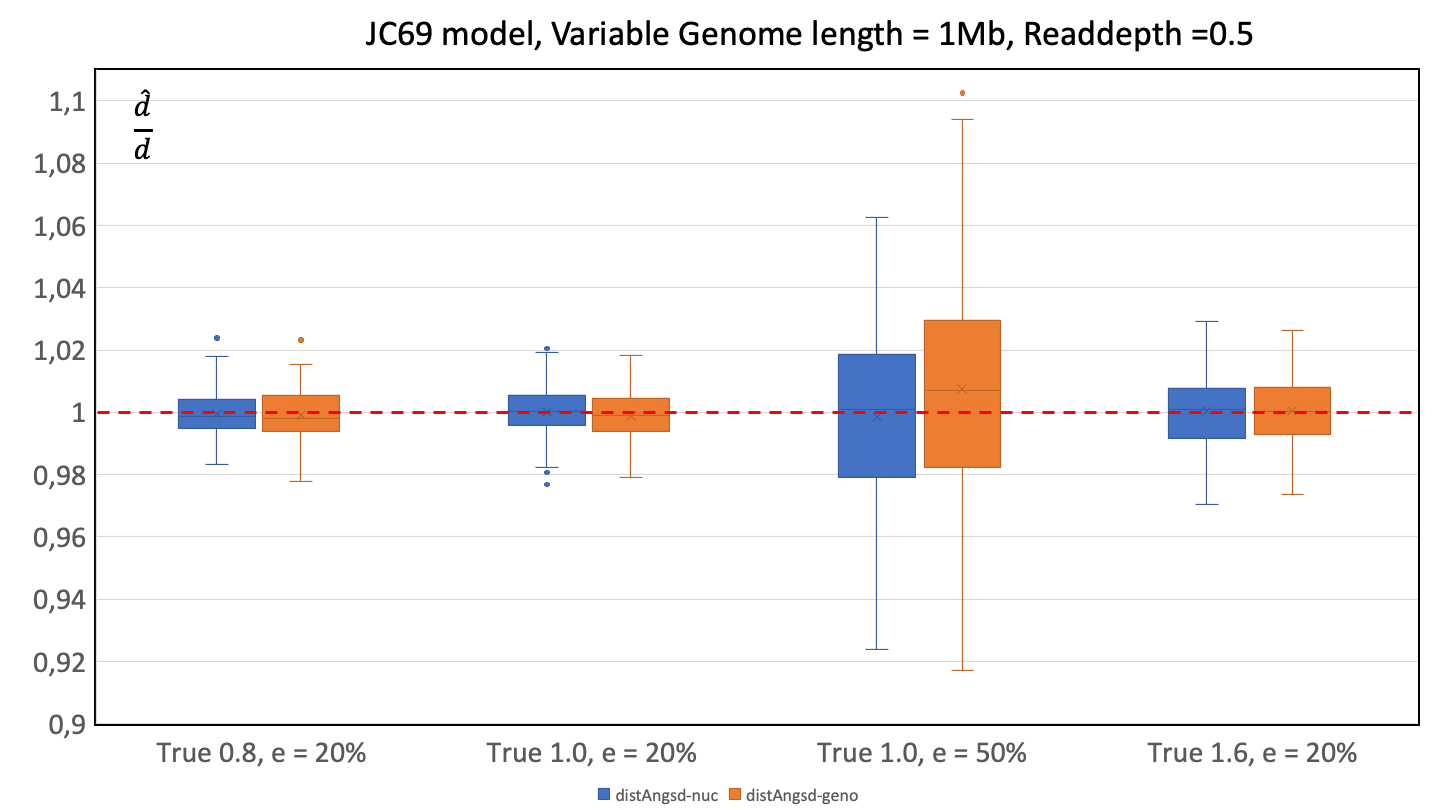
\includegraphics[width=.99\linewidth]{BiasJCRD05_1M.png}  
  \caption{}
  \label{fig:BiasJCRD05_1M}
\end{subfigure}
\begin{subfigure}{.5\textwidth}
  \centering
  % include second image
  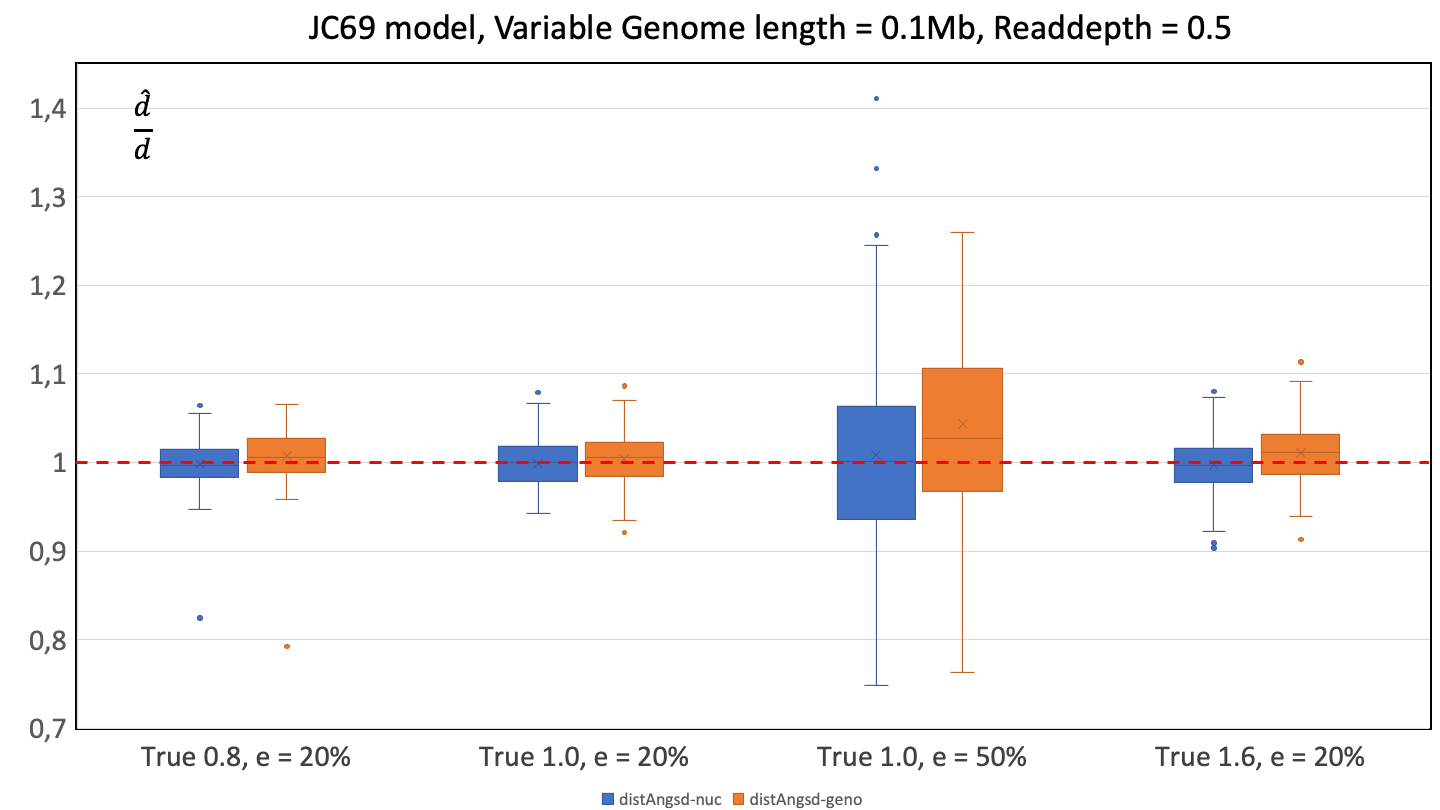
\includegraphics[width=.99\linewidth]{BiasJCRD05_01M.png}  
  \caption{}
  \label{fig:BiasJCRD05_01M}
\end{subfigure}
\newline
\begin{subfigure}{.5\textwidth}
  \centering
  % include first image
  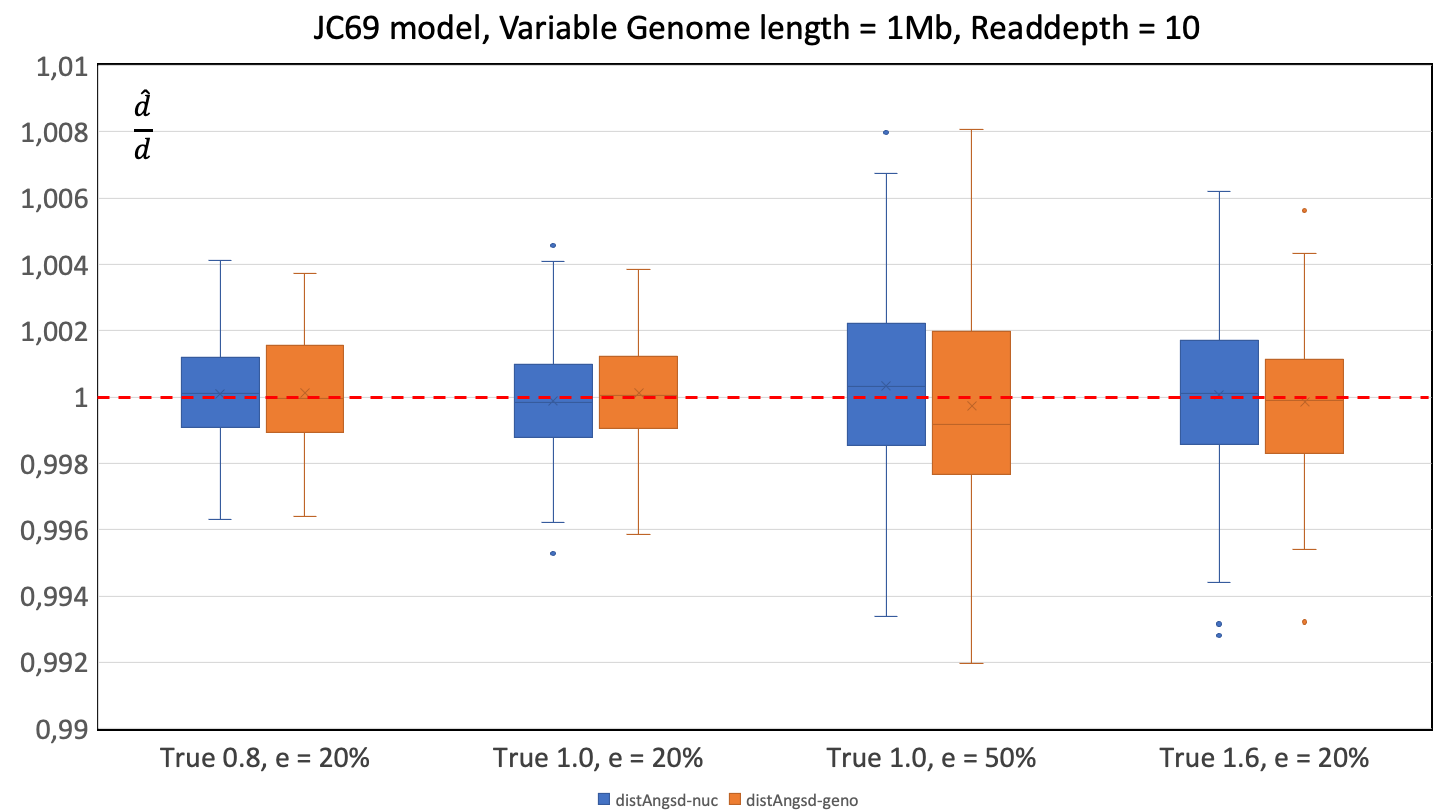
\includegraphics[width=.99\linewidth]{BiasJCRD10_1M.png}  
  \caption{}
  \label{fig:BiasJCRD10_1M}
\end{subfigure}
\begin{subfigure}{.5\textwidth}
  \centering
  % include second image
  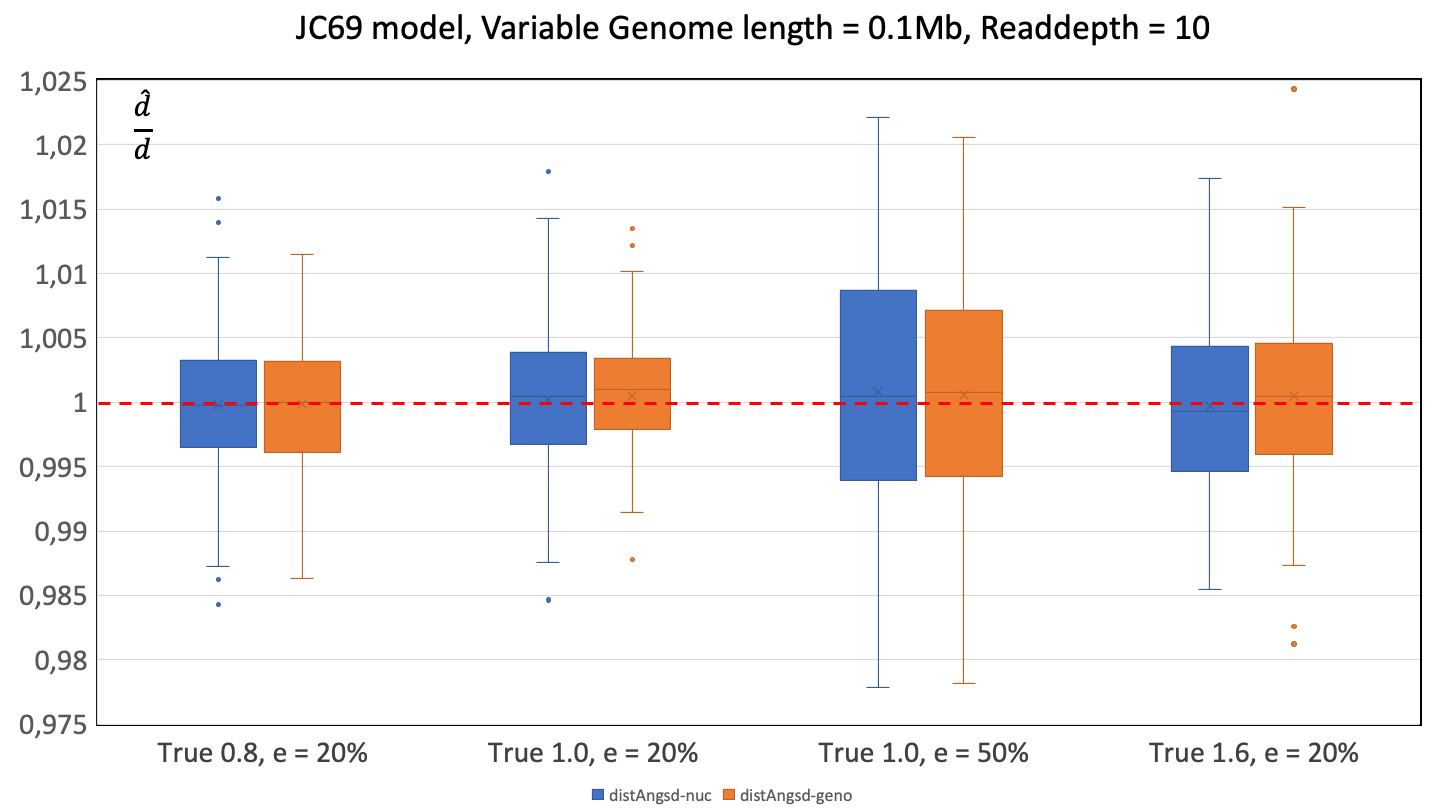
\includegraphics[width=.99\linewidth]{BiasJCRD10_01M.png}  
  \caption{}
  \label{fig:BiasJCRD10_01M}
\end{subfigure}
\caption{Inferred results based on $200$ replicates of JC69 model simulations with different extreme parameter settings to show the evidence of the existence of inferred biases. Simulations follow divergence tree as FIG. 1 in the main text, with $t_1=0.4$ and $t_2 = 0.25$.}
\label{fig:BiasJC}
\end{figure}

\begin{figure}
\begin{subfigure}{.5\textwidth}
  \centering
  % include first image
  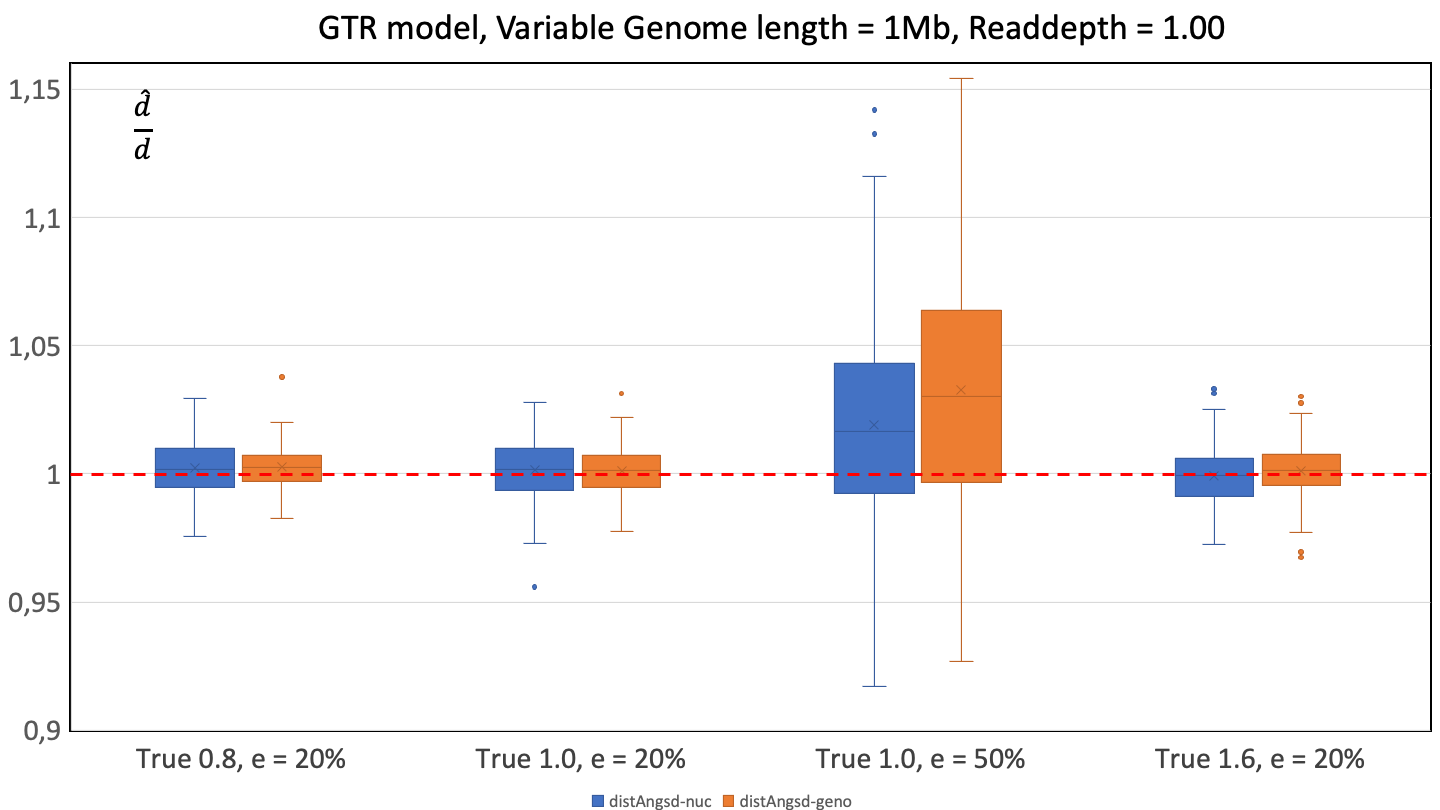
\includegraphics[width=.99\linewidth]{BiasGTRRD1_1M.png}  
  \caption{}
  \label{fig:BiasGTRRD1_1M}
\end{subfigure}
\begin{subfigure}{.5\textwidth}
  \centering
  % include second image
  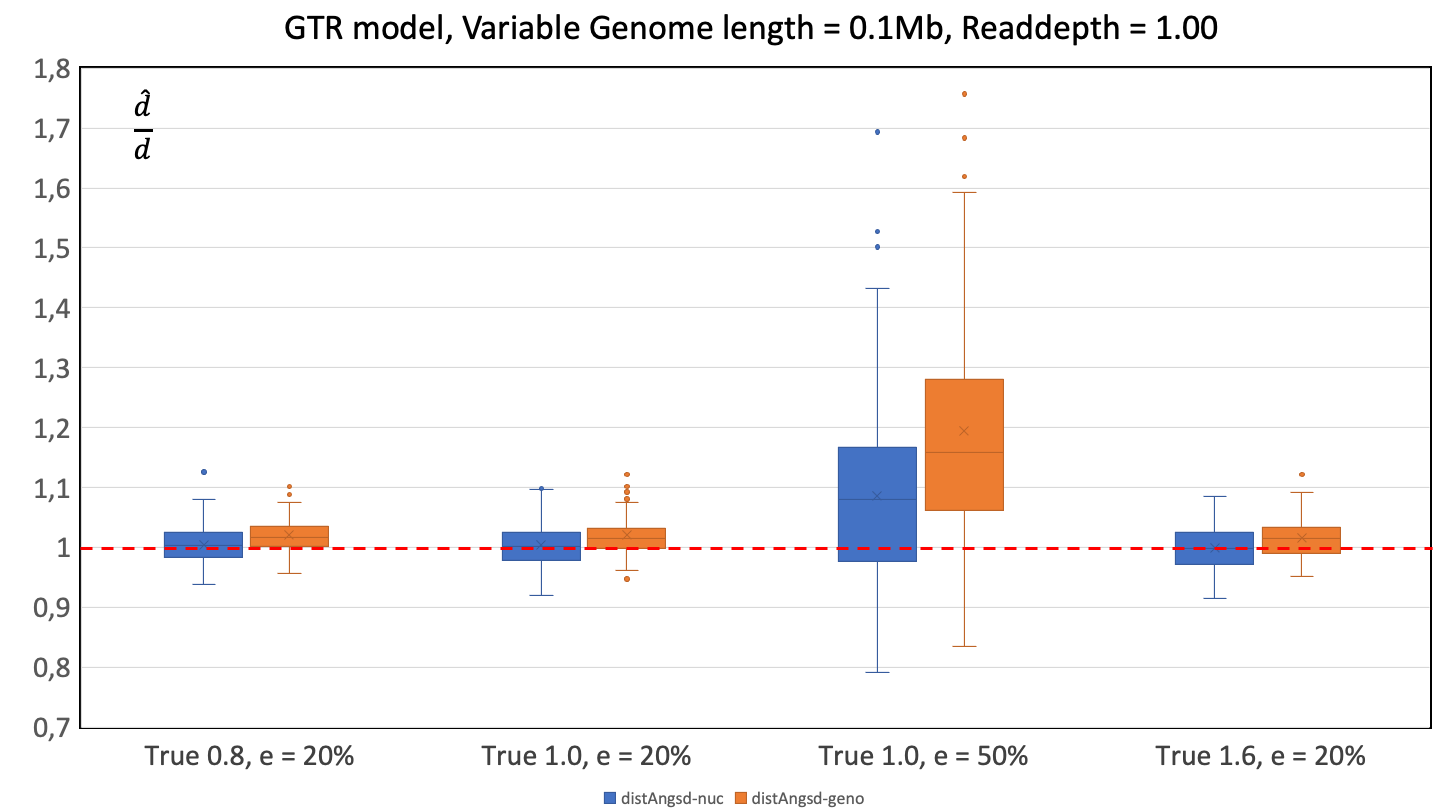
\includegraphics[width=.99\linewidth]{BiasGTRRD1_01M.png}  
  \caption{}
  \label{fig:BiasGTRRD1_01M}
\end{subfigure}
\newline
\begin{subfigure}{.5\textwidth}
  \centering
  % include first image
  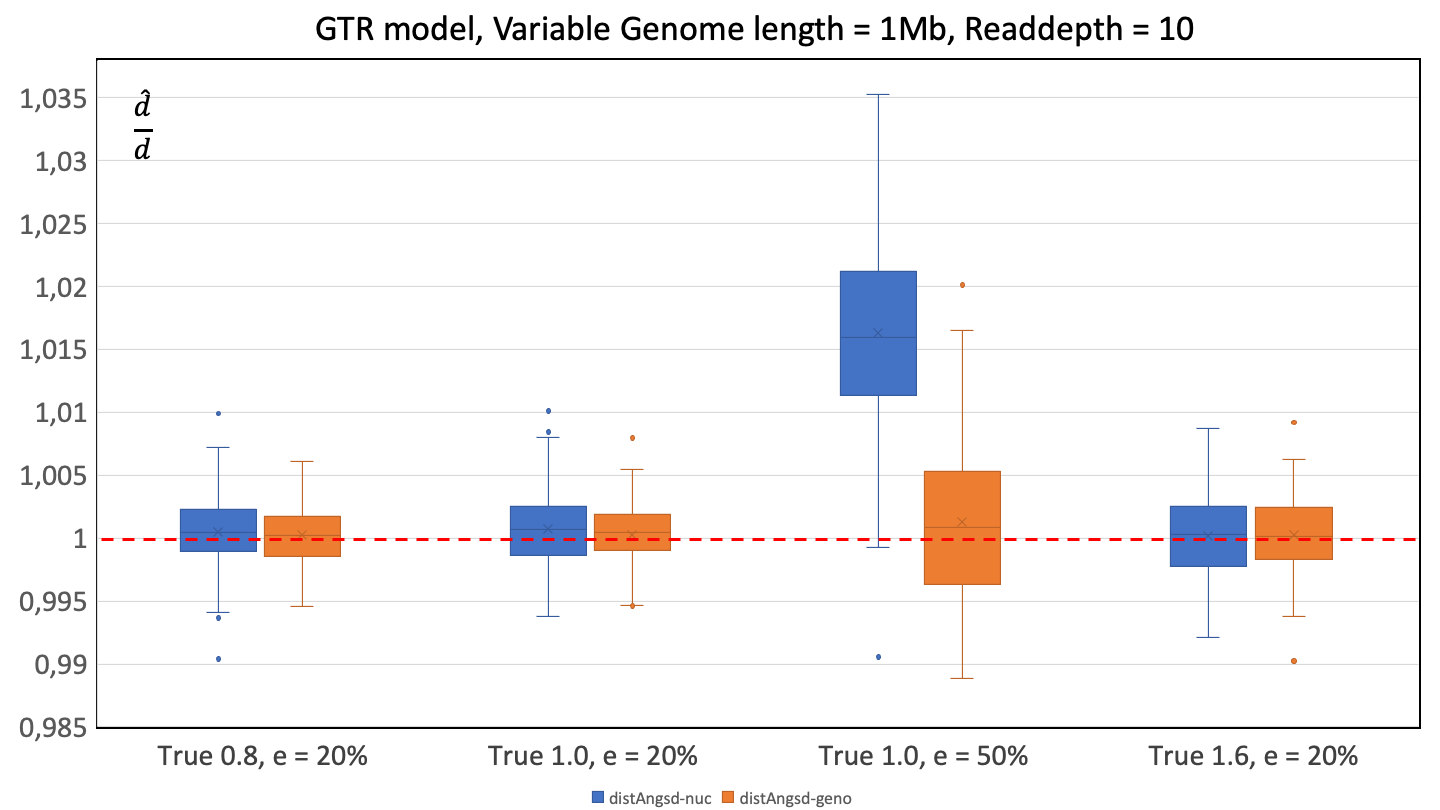
\includegraphics[width=.99\linewidth]{BiasGTRRD10_1M.png}  
  \caption{}
  \label{fig:BiasGTRRD10_1M}
\end{subfigure}
\begin{subfigure}{.5\textwidth}
  \centering
  % include second image
  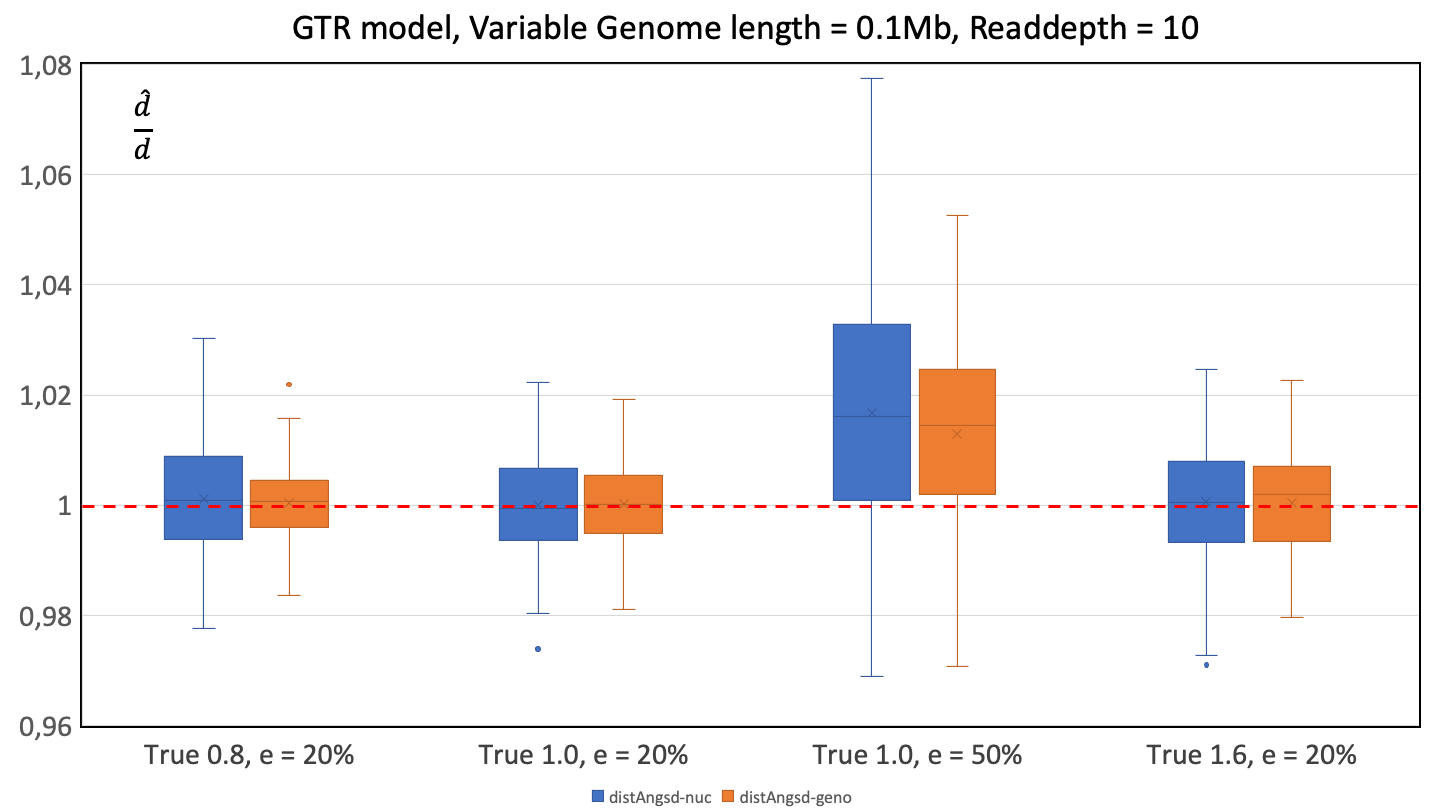
\includegraphics[width=.99\linewidth]{BiasGTRRD10_01M.png}  
  \caption{}
  \label{fig:BiasGTRRD10_01M}
\end{subfigure}
\caption{Inferred results based on $200$ replicates of GTR model simulations with different extreme parameter settings to show the evidence of the existence of inferred biases. Simulations follow divergence tree as FIG. 1 in the main text, with $t_1=0.4$ and $t_2 = 0.25$.}
\label{fig:BiasGTR}
\end{figure}

\section{Pre-existing Methods}
In this section, we will introduce three pre-existing methods for comparison, i.e., RandomSEQ, ConsensusSEQ and ConsensusGT. RandomSEQ refers to the method that one read is randomly chosen per site to infer the genetic distance between individuals. ConsensusSEQ denotes the method that the consensus read (based either on physical read depth or effective base depth \citet{Wang:2013}) per site is used to infer the genetic distance between individuals. And ConsensusGT represents the method that the consensus genotype (according to the posterior distribution given by genotype likelihoods) per site is used to infer the genetic distance between individuals, when the consensus genotype is a heterozygote, ambiguous inference, which will be described below, will be applied. 

We believe for each site of the sample, four pieces of information will contribute to inferring the phylogeny, i.e., the read depth, the base calling errors of each read, the nucleotide frequencies at the site and the ploidy level of the focal organism. All the pre-existing methods together with the proposed distAngsd-geno and distAngsd-nuc methods will take advantage of one or more pieces of information. As shown in Table \ref{tab:Information}, the pre-existing methods make only partially/no use of the base calling errors of each site and other information, while distAngsd-geno uses all the information, and distAngsd-nuc uses all the information except ploidy level. Hence in principle, they should outperform these pre-existing methods.
\begin{table}[ht]
    \centering
    \begin{tabular}{|c|cccc|}
     \hline
      \multirow{2}{*}{Method} & \multicolumn{4}{c|}{Sources of Information}\\
         &Read depth & Base calling errors & Nucleotide frequencies per site & Ploidy level\\
      \hline
      distAngsd-geno & \tickYes & \tickYes & \tickYes & \tickYes\\
      distAngsd-nuc & \tickYes & \tickYes & \tickYes & \tickNo\\
      RandomSEQ & \tickNo & \tickHalfYes & \tickYes & \tickNo\\
      ConsensusSEQ & \tickNo & \tickHalfYes & \tickYes & \tickNo\\
      ConsensusGT & \tickHalfYes & \tickHalfYes & \tickHalfYes & \tickYes\\
      NGSDist & \tickYes & \tickYes & \tickYes & \tickYes\\
      \hline
      \end{tabular}
    \caption{This table shows how different methods make use of the $4$ sources of information to conduct inference. check signs (\tickYes) mean the information is fully used, the cross signs (\tickNo) represent the information is not used, while the semi-check signs (\tickHalfYes) means the information is partially used. \\Since genotype likelihoods are computed by read depth, base calling errors, nucleotide frequencies per site and the prior knowledge of ploidy, and they are fully used by distAngsd-geno. And genotype likelihoods are also partially used by the method ConsensusGT to find the consensus genotype per site, so we mark the columns representing read depth, base calling errors and nucleotide frequencies per sites of ConsensusGT row as semicheck signs. But since ConsensusGT relies on pre-calculated genotype likelihoods, it makes fully use of the information of ploidy level. distAngsd-nuc takes advantage of all the reads and their read quality scores, but it does not use any prior knowledge of ploidy level. If RandomSEQ and ConsensusSEQ use the physical read depths, they only use the information of nucleotide frequencies per site; but if they use the EBD instead, the information of base calling errors are partially taken into account.}
    \label{tab:Information}
\end{table}
\subsection{Ambiguity Inference}
The pre-exsiting methods have problems in handling the samples with large proportion of heterzygous sites, and they treat the sequences in a somewhat
"haploid" way. heterozygous sites within samples are either discarded, or filtered with really restricted criterion. When phylogeny is inferred, any samples will be "compressed" as a single sequence regardless of its ploidy, and homogenous sites will be recognized as a single nucleotide base, i.e., A, C, G, or T; while the remaining heterozygous sites will be written as IUPAC codes. The ambiguity inference methods view a heterozygous genotype at a site as an undetermined base with equal chance to be either of its nucleotides, e.g., the genotype AC is denoted as IUPAC code M and will have 50\% chances to be A or C in calculation. The joint probabilities of genotypes at the same site of the samples with genetic distance $d$ are expressed in Table \ref{tab:Amb}. If the proportion of heterozygous sites is large, the ambiguous methods will underestimate the genetic distance $d$. 

We take $\mathrm{P}_{ij,kl}^{\mathrm{GTR}}(d)$ as an example to show how to derive Table \ref{tab:Amb} based on the GTR model assumption. If the phylogeny is the same as Figure 3 in the main text, A and B share the MRCA (most recent common ancestor) which is of genetic distance $d_1$ from sample $ij$, and of $d_2$ from sample $kl$, and we will have $ij$ and $kl$ is of distance $d = d_1+d_2$. According to the GTR model properties, we have
\begin{align*}
    \mathrm{P}_{ij,kl}^{\mathrm{GTR}}(d)&=\sum_{m\in\{{\rm A,C,G,T}\}}\pi_{m}\left(\frac{1}{2}\mathrm{P}_{m,i}(d_1)+\frac{1}{2}\mathrm{P}_{m,j}(d_1)\right)\left(\frac{1}{2}\mathrm{P}_{m,k}(d_2)+\frac{1}{2}\mathrm{P}_{m,l}(d_2)\right)\\
    &=\frac{1}{4}\sum_{m\in\{{\rm A,C,G,T}\}}\left(\pi_i\mathrm{P}_{i,m}(d_1)+\pi_j\mathrm{P}_{j,m}(d_1)\right)\left(\mathrm{P}_{m,k}(d_2)+\mathrm{P}_{m,l}(d_2)\right)\\
    &=\frac{1}{4}\mathrm{\pi}_i\left[\mathrm{P}_{i,k}(d)+\mathrm{P}_{i,l}(d)\right]+\frac{1}{4}\mathrm{\pi}_j\left[\mathrm{P}_{j,k}(d)+\mathrm{P}_{j,l}(d)\right],
\end{align*}
which corresponds to the last row of Table \ref{tab:Amb}. And all the other rows' results in the table can also be derived in the similar way. 
% It is based on a wrong model: it tries to infer the $t_div$ between the internal nodes A and B.
% And the likelihoods given above can be viewed as joint distribution of nucleotides at A and B. 
% (When substitution rate is so small that the times from A/B to tips are not sufficient to carry
% substitutions, one can view the the distribution of nucleotides at A as half $i$ half $j$, and the one of B as half $k$ half $l$). However, when the substitution rate or the the times from A/B to tips are large enough, the distributions of nucleotides at A and B can not be approximated as above. 

\begin{table}[h]
\centering
 \begin{tabular}{|P{0.001cm}|P{1.6cm}|P{7cm}|} 
 \hline\xrowht[()]{15pt}
 & Denotation & Ambiguous inference likelihood  \\  
 \hline\xrowht[()]{15pt} 
 &$\mathrm{P}_{ii,ii}^{\mathrm{GTR}}(d)$ & $\mathrm{\pi}_i\mathrm{P}_{i,i}(d)$  \\  
 \hline\xrowht[()]{15pt} 
 &$\mathrm{P}_{ii,ij}^{\mathrm{GTR}}(d)$ & $\frac{1}{2}\mathrm{\pi}_i\left[\mathrm{P}_{i,i}(d)+\mathrm{P}_{i,j}(d)\right]$  \\\hline\xrowht[()]{15pt} 
 &$\mathrm{P}_{ij,ij}^{\mathrm{GTR}}(d)$ & $\frac{1}{4}\mathrm{\pi}_i\left[\mathrm{P}_{i,i}(d)+\mathrm{P}_{i,j}(d)\right]+\frac{1}{4}\mathrm{\pi}_j\left[\mathrm{P}_{j,i}(d)+\mathrm{P}_{j,j}(d)\right]$ \\
 \hline\xrowht[()]{15pt}
 &$\mathrm{P}_{ii,jj}^{\mathrm{GTR}}(d)$ & $\mathrm{\pi}_i\mathrm{P}_{i,j}(d)$ \\
 \hline\xrowht[()]{15pt}
 &$\mathrm{P}_{ii,jk}^{\mathrm{GTR}}(d)$ & $\frac{1}{2}\mathrm{\pi}_i\left[\mathrm{P}_{i,j}(d)+\mathrm{P}_{i,k}(d)\right]$  \\
 \hline\xrowht[()]{15pt}
 &$\mathrm{P}_{ij,ik}^{\mathrm{GTR}}(d)$ & $\frac{1}{4}\mathrm{\pi}_i\left[\mathrm{P}_{i,i}(d)+\mathrm{P}_{i,k}(d)\right]+\frac{1}{4}\mathrm{\pi}_j\left[\mathrm{P}_{j,i}(d)+\mathrm{P}_{j,k}(d)\right]$ \\
 \hline\xrowht[()]{15pt}
 &$\mathrm{P}_{ij,kl}^{\mathrm{GTR}}(d)$ & $\frac{1}{4}\mathrm{\pi}_i\left[\mathrm{P}_{i,k}(d)+\mathrm{P}_{i,l}(d)\right]+\frac{1}{4}\mathrm{\pi}_j\left[\mathrm{P}_{j,k}(d)+\mathrm{P}_{j,l}(d)\right]$ \\
 \hline
\end{tabular}
%  \begin{tabular}{|c | c| c|} 
%  \hline
%   & Ambiguous inference likelihood & 2DSFS inference likelihood \\ [0.5ex] 
%  \hline
%  $\mathrm{P}_{ii,ii}(d)$ & $\mathrm{\pi}_i\mathrm{P}_{i,i}(d)$ & $\left[\mathrm{\pi}_i\mathrm{P}_{i,i}(d)\right]^4$  \\ 
%  \hline
%  $\mathrm{P}_{ii,ij}(d)$ & $\frac{1}{2}\mathrm{\pi}_i\left[\mathrm{P}_{i,i}(d)+\mathrm{P}_{i,j}(d)\right]$ & $\left[\mathrm{\pi}_i\mathrm{P}_{i,i}(d)\right]^2\left[\mathrm{\pi}_i\mathrm{P}_{i,j}(d)\right]^2$ \\
%  \hline
%  $\mathrm{P}_{ij,ij}(d)$ & $\frac{1}{4}\mathrm{\pi}_i\left[\mathrm{P}_{i,i}(d)+\mathrm{P}_{i,j}(d)\right]+\frac{1}{4}\mathrm{\pi}_j\left[\mathrm{P}_{j,i}(d)+\mathrm{P}_{j,j}(d)\right]$ & $\left[\mathrm{\pi}_i\mathrm{P}_{i,i}(d)\right]\left[\mathrm{\pi}_i\mathrm{P}_{i,j}(d)\right]\left[\mathrm{\pi}_j\mathrm{P}_{j,i}(d)\right]\left[\mathrm{\pi}_j\mathrm{P}_{j,j}(d)\right]$\\
%  \hline
%  $\mathrm{P}_{ii,jj}(d)$ & $\mathrm{\pi}_i\mathrm{P}_{i,j}(d)$ & $\left[\mathrm{\pi}_i\mathrm{P}_{i,j}(d)\right]^4$ \\
%  \hline
%  $\mathrm{P}_{ii,jk}(d)$ & $\frac{1}{2}\mathrm{\pi}_i\left[\mathrm{P}_{i,j}(d)+\mathrm{P}_{i,k}(d)\right]$ & $\left[\mathrm{\pi}_i\mathrm{P}_{i,j}(d)\right]^2\left[\mathrm{\pi}_i\mathrm{P}_{i,k}(d)\right]^2$ \\
%  \hline
%  $\mathrm{P}_{ij,ik}(d)$ & $\frac{1}{4}\mathrm{\pi}_i\left[\mathrm{P}_{i,i}(d)+\mathrm{P}_{i,k}(d)\right]+\frac{1}{4}\mathrm{\pi}_j\left[\mathrm{P}_{j,i}(d)+\mathrm{P}_{j,k}(d)\right]$ & $\left[\mathrm{\pi}_i\mathrm{P}_{i,i}(d)\right]\left[\mathrm{\pi}_i\mathrm{P}_{i,k}(d)\right]\left[\mathrm{\pi}_j\mathrm{P}_{j,i}(d)\right]\left[\mathrm{\pi}_j\mathrm{P}_{j,k}(d)\right]$\\
%  \hline
%  $\mathrm{P}_{ij,kl}(d)$ & $\frac{1}{4}\mathrm{\pi}_i\left[\mathrm{P}_{i,k}(d)+\mathrm{P}_{i,l}(d)\right]+\frac{1}{4}\mathrm{\pi}_j\left[\mathrm{P}_{j,k}(d)+\mathrm{P}_{j,l}(d)\right]$ & $\left[\mathrm{\pi}_i\mathrm{P}_{i,k}(d)\right]\left[\mathrm{\pi}_i\mathrm{P}_{i,l}(d)\right]\left[\mathrm{\pi}_j\mathrm{P}_{j,k}(d)\right]\left[\mathrm{\pi}_j\mathrm{P}_{j,l}(d)\right]$\\
%  \hline
% \end{tabular}
\caption{The joint probabilities of genotypes at the same site of the samples with genetic distance $d$ on which the ambiguity inference methods are based. The molecular evolution model is assumed to be GTR.}
\label{tab:Amb}
\end{table}

For the more general GTR+I model, the ambiguity inference method, we will have,
\begin{align*}
\mathrm{P}_{ij,kl}^{\mathrm{GTR+I}}(d)=\left(1-p_{inv}\right)\mathrm{P}_{ij,kl}^{\mathrm{GTR}}(d)+p_{inv}\delta_{i=j=k=l}
\end{align*}

\section{Phred2D implement}
As the bcftools calculates Phred-scaled genotype likelihoods, the genotype likehoods are stored as integers and inevitably lose some precisions. When dealing with data downstream bcftools treatments, keeping a high precision is not necessary, we thus store the genotype likehoods in the format of unsigned char while coding, which occupies $8$ bits rather than $32$ bit as of float or $64$ bit as of double. Unsigned char can naturally converted into an integer ranging from $0$ to $255$, which is used to represent the Phred-scaled genotype likehood (PL) (If $\mathrm{PL}>255$ which means $\mathrm{GL}<10^{-25.5}$, we will set $\mathrm{PL}=255$).

Note that in the Equation \ref{eq:Miteration}, it is the product of two genotype likehoods, i.e., $\mathrm{GL}_1^s(g_1)\mathrm{GL}_2^s(g_2)$, rather than the single likelihood that matters. And the unsigned char Phred-scaled genotype likelihood can only take $256$ values, $\mathrm{GL}_1^s(g_1)\mathrm{GL}_2^s(g_2)$ can take $256+\frac{256\times 255}{2}=32896$ discrete values, which can be pre-calculated and stored in a $256\times 256$ matrix.

By implement the unsigned char storage of genotype likelihoods and pre-calculate all possible values of the product of two genotype likehoods, we can largely save both computational time and memory without losing precisions downstream the current bcftools treated data. Since the pre-calculated Phred-scaled genotype likelihood products are stored in a 2D matrix, we call this method the Phred2D implement.

\section{Oak data}
The proposed distAngsd-geno method is applied to inferring the phylogeny of the published oak dataset (\cite{Fitz-Gibbon_Hipp_Pham_Manos_Sork:2017}). There are RADseq sequences from $83$ oak samples representing $16$ taxa across the US. The data was aligned to a collapsed version of reference genome (v0.5, \cite{Sork:2016}; available from \url{https://valleyoak.ucla.edu/genomicre sources/}) via BWA-MEM v.0.7.17 (\cite{Li:2013}). VCFtools v.0.1.17 (\cite{Danecek:2011}) was then applied to calculate the genotype likelihoods and get the .vcf files. The bed file of sites passing the filtering criteria in \cite{Fitz-Gibbon_Hipp_Pham_Manos_Sork:2017} of each sample was kindly shared by Dr. Fitz-Gibbon and Prof. Sork to gurantee that we are on the right track to conduct phylogeny inference. Their filtering criteria and adjustments in are as follows,
\begin{enumerate}[i]
    \item Identification of targeted genome regions and variant discovery were done with GATK v3.6-0-g89b7209 (McKenna et al. 2010), as follows. We ran CallableLoci on each sample with default parameters, except that minimum read depth was set to 5 and maximum read depth was set to 100 (minDepth 5 and maxDepth 100). An overall set of callable regions, hereafter referred to as reference-mapped loci, included all regions of exactly 86 bp determined to be callable in at least four samples. HaplotypeCaller variant discovery was run using emitRefConfidence GVCF mode separately for each sample. The whole cohort was concurrently genotyped over the reference-mapped loci regions using GenotypeGVCFs with a minimum confidence of 30.
    \item Based on inspection of variant calls and read alignments (Robinson et al. 2011), we chose to only filter the variants by QD as well as requiring them to be biallelic. VariantFiltration was used to apply a QD $< 2.0$ filter tag. 
    \item VCFtools v0.1.15 (Danecek et al. 2011) was used to filter non-biallelic variants. 
    \item Sites with filtered variants, including non-biallelic variants were converted to Ns for all samples (these sites are filtered out later by the phylogenic analysis software).
    \item For each sample, GATK loci not considered callable by the above CallableLoci step were converted to Ns.
    \item Sequences were printed with passing variants applied according to homozygous genotype or if heterozygous IUPAC ambiguity codes were used.
    \item Homozygous indel variants were included using dashes to maintain the overall alignment. However, there is no IUPAC ambiguity code for heterozygous indels and so they were instead encoded as Ns.
\end{enumerate}
Apart from the filtering and adjustments described above, The bed files of sites they sent to us also go through an extra round of filtering to remove the loci with more than five heterozygous sites, but as they pointed out later that "the extra filters had little effect on phylogeny topology or congruence although the relative positions of the Q. lobata and Q. engelmannii clades were altered, but with zero bootstrap support".

The filters described above had largely suppressed the fraction of heterozygous sites in the downstream phylogeny analyses, and the remaining heterozygous sites will be treated as IUPAC ambiguity codes due to the limitations of the pre-existing methods. In order to recover more heterozygous sites (non-biallelic sites) and uncertainties (low quality sites) which distAngsd-geno is believed to handle, we only used the information of positions of loci in each bed file. And for the marked Ns within the loci regions which has mapped reads information, we restored them. For every pair of oak samples, the parallel-computatinal distAngsd-geno inference with simplest JC69 model was conducted and only the sites with non-zero read depths for both samples will be used to estimate the pairwise genetic distances.  Once the $83\times 83$ pairwise matrix is determined, program PhyD (\cite{Criscuolo:2008}) will use the BioNJ (\cite{Gascuel:1997}) algorithm to build neighbour joining trees, and trees were plotted with FigTree v1.4.4. (\url{http://tree. bio.ed.ac.uk/software/figtree/}). 

As distAngsd-geno is currently implemented for pairwise genetic distance inference and the simplest JC69 model was used for the inference of the real data, it is not very suitable to directly compare the distAngsd-geno's results with the results in the original paper (\cite{Fitz-Gibbon_Hipp_Pham_Manos_Sork:2017}) where they conducted such inferences based on ML tree with more complicated model, we thus compared our inference results with pre-existing methods based sorely on JC69 model, i.e., ConsensusSEQ and ConsensusGT. Bcftools consensus was applied to getting the consensus nucleotide sequence and the consensus genotype sequence of each sample. And the putative heterozygous sites in ConsensusGT were expressed as IUPAC codes. Then the pairwise distances between samples were calculated as the genetic distance between their consensus sequences based on the JC69 model. The following figure is a comparison between phylogeny trees of $83$ oaks inferred by distAngsd-geno, ConsensusSEQ and ConsensusGT.

From the appearances of the trees in FIG. \ref{fig:OakTree}, it seems that the distAngsd-geno tree can group the $83$ oak samples better compared with the other two trees, as it gives clearest boundaries between {\it Quercus berberidifolia}, {\it Quercus durata var. gabrielensis
} and {\it Quercus durata var. durata}. 

\begin{figure*}[h]
    \centering
    \begin{subfigure}[b]{0.95\textwidth}
    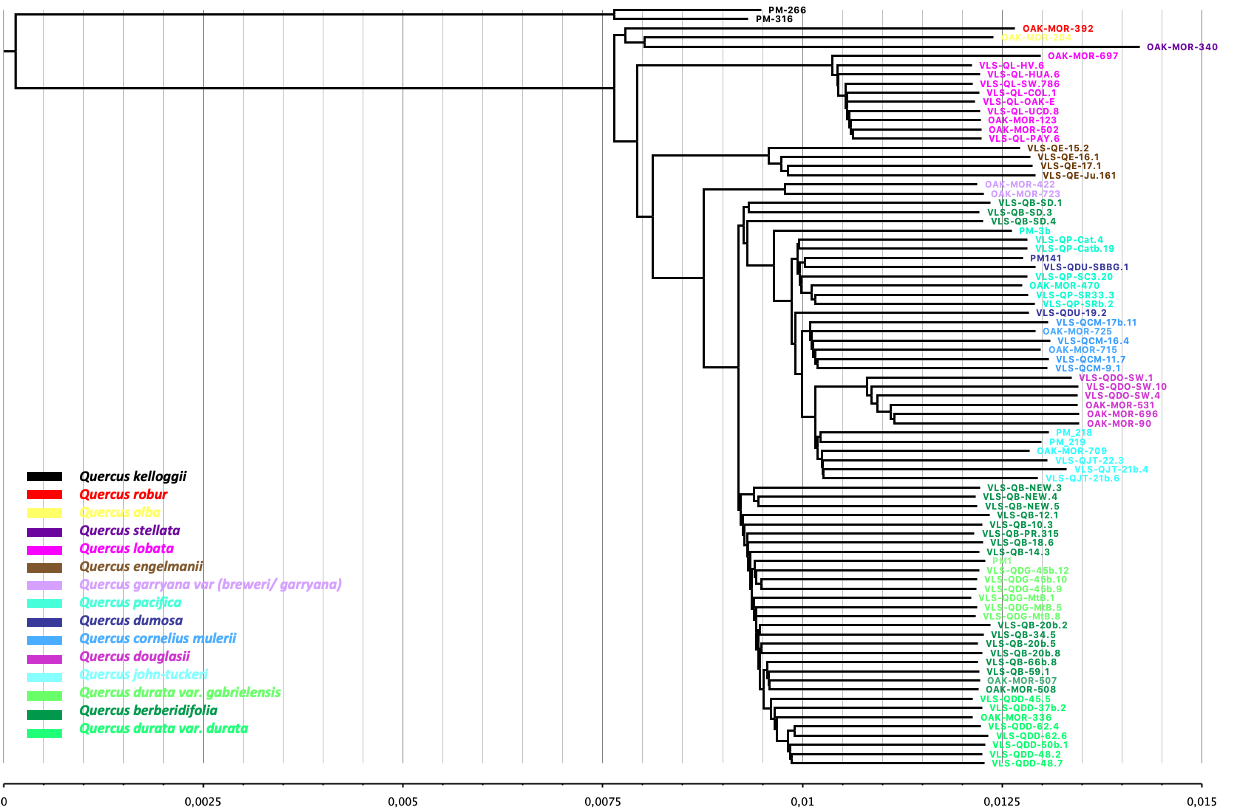
\includegraphics[width=\textwidth]{matrix_full_nofiltering.in_bionj.t1.png}
    \caption{distAngsd-geno inferred tree}
    \label{fig:distAngsd-genoOakTree}
    \end{subfigure}
    \begin{subfigure}[b]{0.95\textwidth}
    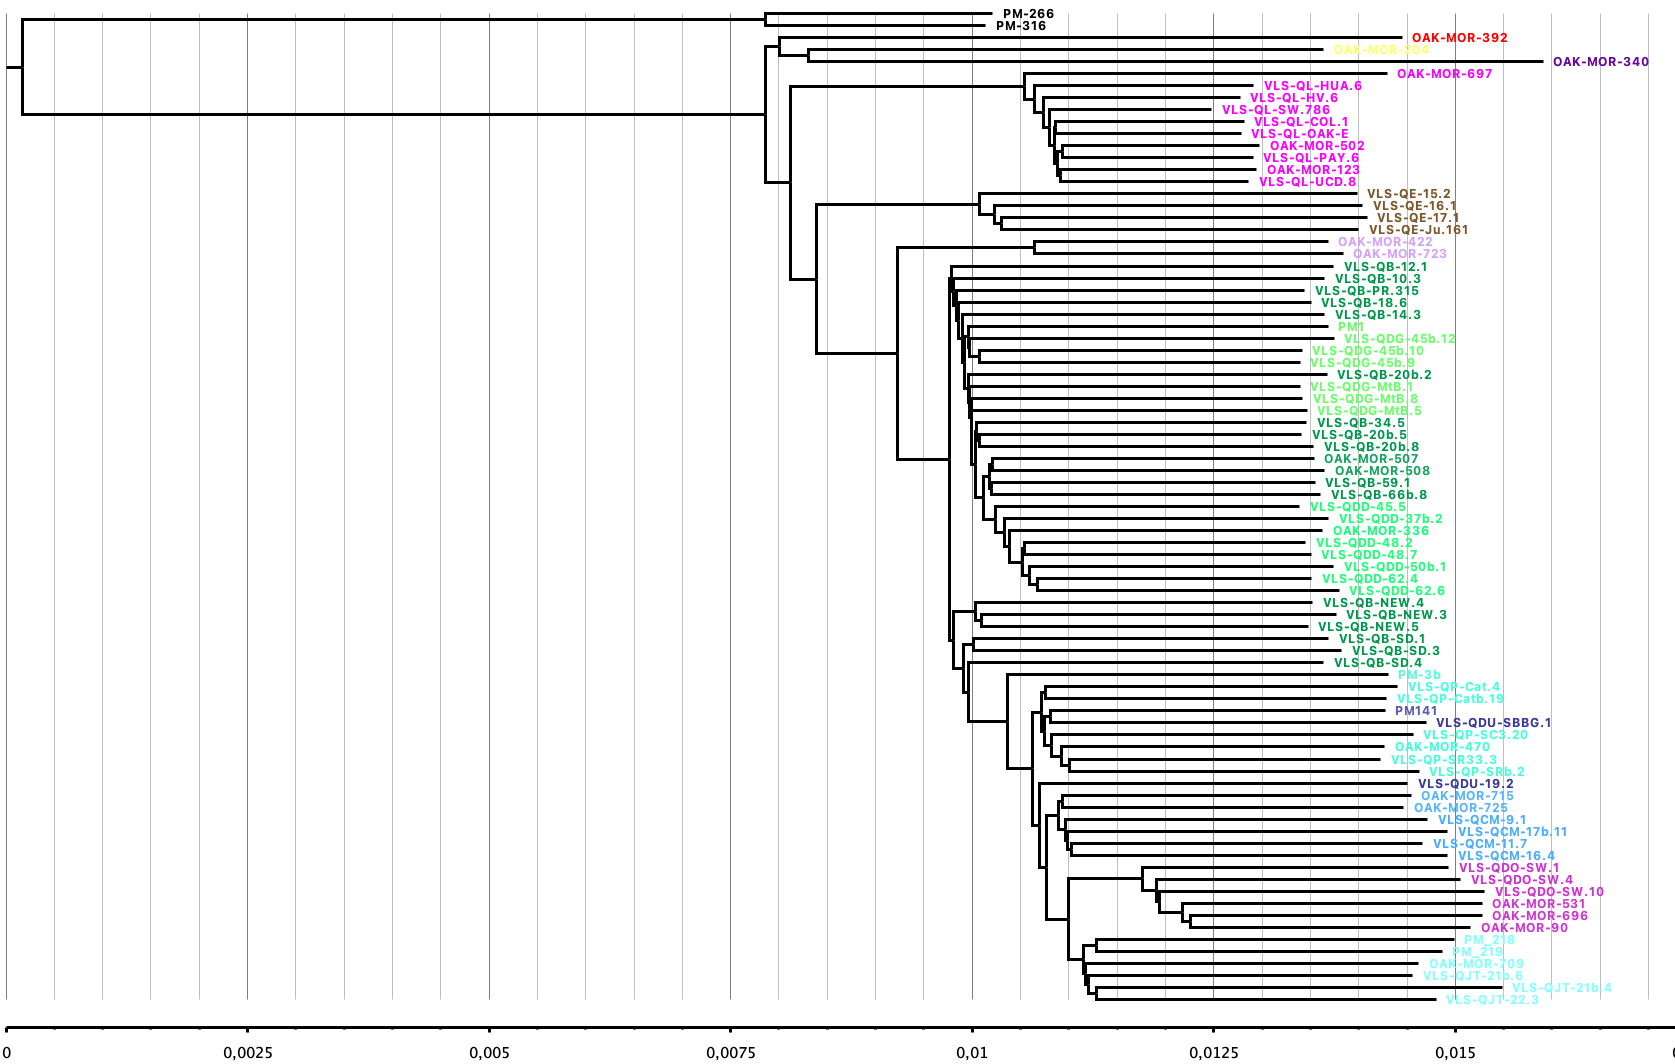
\includegraphics[width=\textwidth]{JCAmatrix_full_nofiltering_SEQ.in_bionj.t.png}
    \caption{ConsensusSEQ inferred tree}
    \label{fig:ConsensusSEQOakTree}
    \end{subfigure}
\end{figure*}
\begin{figure*}[ht]\ContinuedFloat
    \begin{subfigure}[b]{0.95\textwidth}
    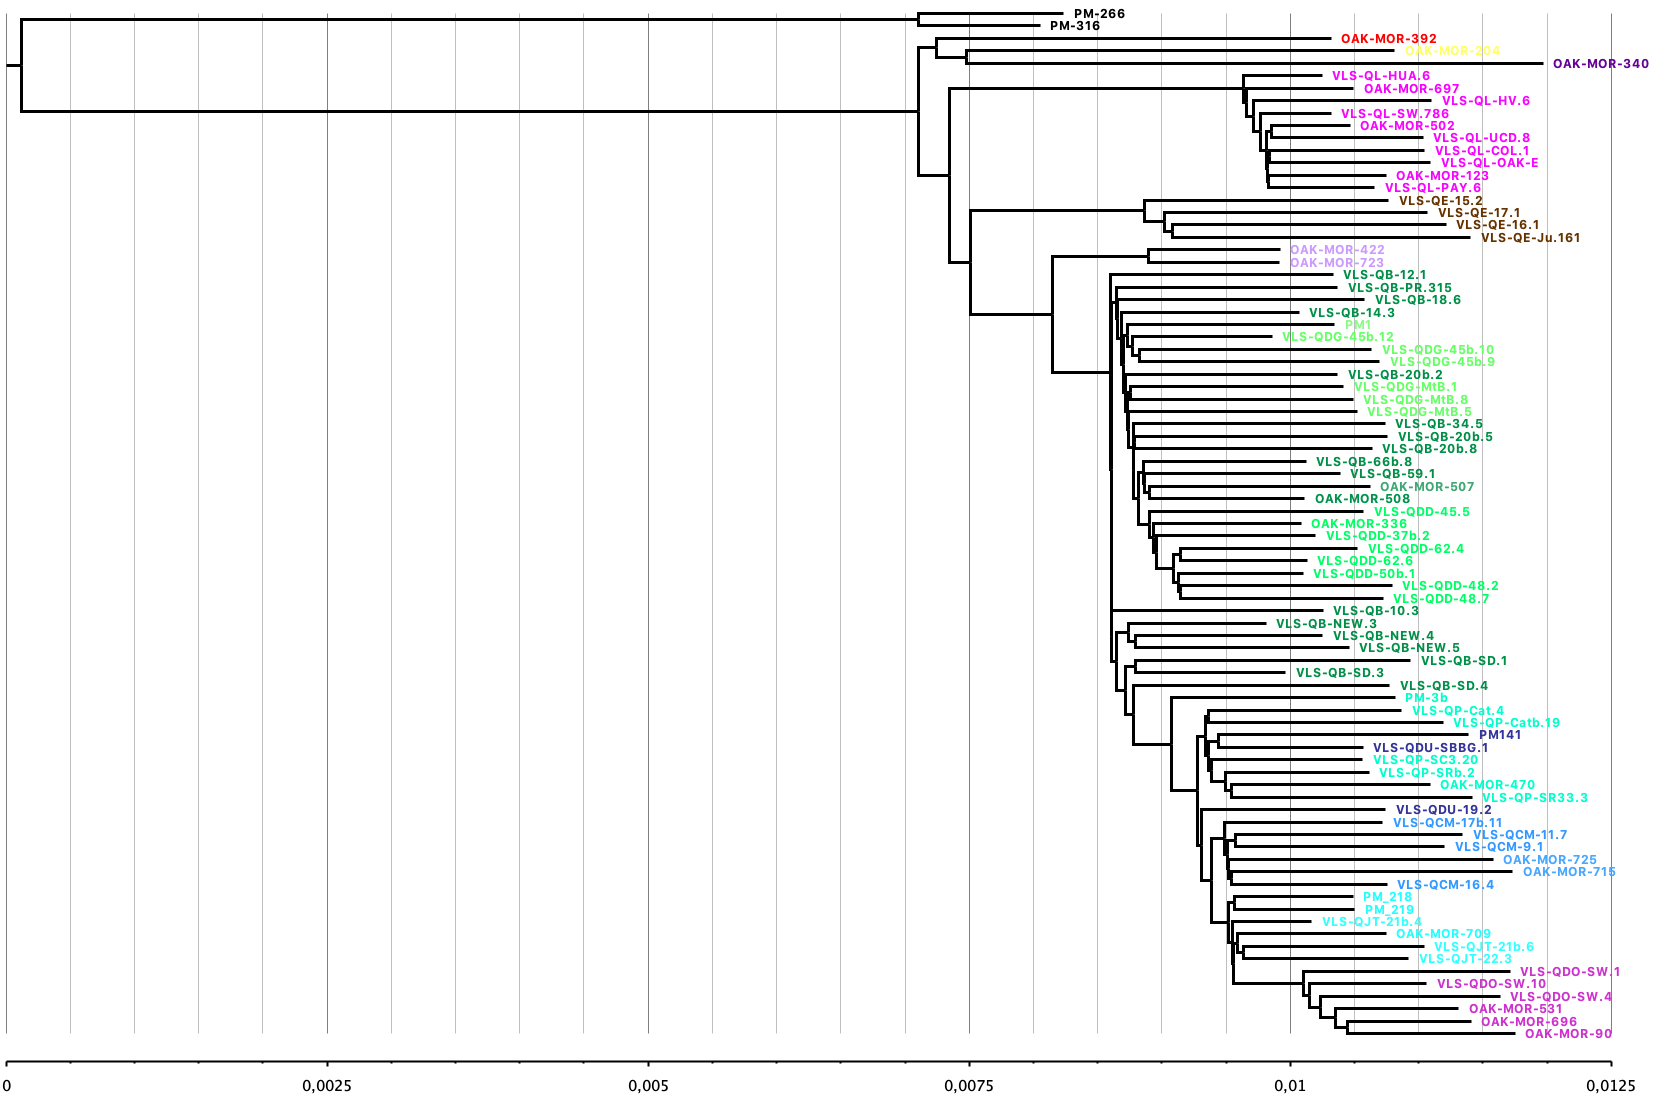
\includegraphics[width=\textwidth]{JCAmatrix_full_nofiltering.in_bionj.t.png}
    \caption{ConsensusGT inferred tree}
    \label{fig:ConsensusGTOakTree}
    \end{subfigure}
    \vspace{0.5cm}
    \caption{Neighbour-Joining Tree of $83$ oak inferred by (a) distAngsd-geno method (b) ConsensusSEQ method, and (c) ConsensusGT method. All these inferences are based on the JC69 model, the colors of the labeled names represent the species shown in the legend. The trees are all inferred by the full data rather than the downsampled data. All three trees are actually unrooted trees with roots placed between the known outgroup {\it Quercus kelloggii} and other Oak species.}
    \label{fig:OakTree}
\end{figure*}

All trees in FIG. \ref{fig:OakTree} are based on the full data which are the original $83$ oak samples with mean read depth $20.32$ (per sample) and lowest depth $10.34$. To further confirm this conclusion and test the inference capability of the new method when low coverage is observed, we conduct downsampling procedures to each sample by samtools view -s command and obtain the samples with mean read depth per site $10$, $5$, $1$, $0.75$, $0.5$ and $0.25$. All downsampled data with same level of mean depths are used to infer a Neighbour-Joining tree via distAngsd-geno method, ConsensusSEQ method and ConsensusGT method. And a compatibility measurement $m$ is developed (See in Supplementary Information) to check how well the inferred trees go with the prior species knowledge obtained from \cite{Fitz-Gibbon_Hipp_Pham_Manos_Sork:2017}. Table \ref{tab:DownsamplingExperimentalResults} shows the $m$ values of different trees with different mean depths based on different methods.

\begin{table*}[ht]
    \centering
    \begin{tabular}{|c|c|c|ccccccc|}
     \hline
     \multirow{4}{*}{Criterion $|\Omega_1\cap \Omega_2|=0$}& \multicolumn{2}{c|}{Downsampling depth} & full & $10$ & $5$ & $1$ & $0.75$ & $0.5$ & $0.25$\\
      \cline{2-10}
      & distAngsd-geno & \multirow{3}{*}{$m$} & 17 & 17 & 17 & 16 & 16 & 17 & 13 \\
      & ConsensusSEQ & & 17 & 17 & 17 & 16 & 16 & 16 & 13\\
      & ConsensusGT & & 16 & 16 & 16 & 16 & 16 & 16 & 12\\
      \hline
      \multirow{4}{*}{Criterion $|\Omega_1\cap \Omega_2|\leq 1$} &\multicolumn{2}{c|}{Downsampling depth} & full & $10$ & $5$ & $1$ & $0.75$ & $0.5$ & $0.25$\\
      \cline{2-10}
       & distAngsd-geno &\multirow{3}{*}{$m$} & 75 & 75 & 73 & 74 & 73 & 70 & 57 \\
      & ConsensusSEQ & & 74 & 75 & 76 & 72 & 70 & 66 & 58\\
      & ConsensusGT & & 75 & 75 & 74 & 74 & 70 & 67 & 56\\
    \hline
      \end{tabular}
    \caption{The compatibility measurement $m$ between the inferred pairwise distance trees and the prior species knowledge.The trees are inferred based on the original samples as well as the downsampled samples. The original 83 samples have mean read depth $20.32$ with lowest depth $10.34$, and each sample is downsampled to mean read depth $10$, $5$, $1$, $0.75$, $0.5$ and $0.25$.}
    \label{tab:DownsamplingExperimentalResults}
\end{table*}

The larger the compatibility measurement $m$ is, the better the tree go with the prior species knowledge. Table \ref{tab:DownsamplingExperimentalResults} can further validate that distAngsd-geno tree is better than both ConsensusSEQ and ConsensusGT trees when read depth is lower.

\section{Compatibility measurement between the tree and the prior knowledge}
%We introduce a compatibility measurement between the inferred tree and the prior knowledge. 
Assume that we have prior knowledge about the leave node samples belong to which species, and we want to evaluate how compatible the inferred phylogenetic tree with the prior knowledge. Since different methods may measure genetic distances with different scales and different models, it is not suitable to compare the absolute/relative pairwise distances between inferred trees. Hence we introduce a compatibility measurement $m$ between the tree and the prior knowledge.

Since we have the prior knowledge of the groups (species/subspecies) that each leaf node belongs to, leaves are marked with the names of their groups (as A, B and C in FIG. \ref{fig:topologicaltree}). For a binary unrooted tree with fixed number of leave node $n$, there will be $(n-3)$ internal branches. As shown in FIG. \ref{fig:topologicaltree}, a tree with $5$ leaves has $2$ internal branches, i.e., $\alpha$ and $\beta$.  Once a specific internal branch is cut off, two subtrees will naturally be formed. The leaves of both subtrees will correspondingly form two sets, i.e., $\Omega_1$ and $\Omega_2$. For instance, if branch $\alpha$ of Tree 1 is cut off in FIG. \ref{fig:topologicaltree}, $\Omega_1=\{\mathrm{A}\}$ and $\Omega_2=\{\mathrm{B,C}\}$, similarly if $\beta$ of Tree 1 is cut off, $\Omega_1=\{\mathrm{A,C}\}$ and $\Omega_2=\{\mathrm{B}\}$; while $\Omega_1$ and $\Omega_2$ can always be defined as $\{\mathrm{A,B}\}$ and $\{\mathrm{A,B,C}\}$ if either branch $\alpha$ or $\beta$ of Tree 2 is cut off; if branch $\alpha$ of Tree 3 is cut off, $\Omega_1=\{\mathrm{A,C}\}$ and $\Omega_2=\{\mathrm{A,B}\}$, and if $\beta$ of Tree 3 is cut off, $\Omega_1=\{\mathrm{A,C}\}$ and $\Omega_2=\{\mathrm{B}\}$. The compatibility measurement $m$ between the tree and the prior knowledge is defined as the number of internal branches whose corresponding $\Omega_1$ and $\Omega_2$ satisfy (1) $|\Omega_1 \cap \Omega_2|=0$ or (2) $|\Omega_1 \cap \Omega_2|\leq 1$. The criterion (1) here is to find the internal branches that clearly define the boundary between groups, while the criterion (2) is loosing criterion (1) and trying to find the upper bound of the number of internal branches that not go against the prior knowledge of groups. For both criteria, the larger $m$ is, the better the tree goes well with the prior group knowledge.

If we choose the criterion (1), The compatibility measurement $m$ will be $2$, $0$ and $1$ for Tree 1, Tree 2 and Tree 3 in FIG. \ref{fig:topologicaltree}) correspondingly, while the compatibility measurement $m$ will be $2$, $0$ and $2$ correspondingly if criterion (2) is adopted. Combining the $m$'s values in both criteria, we come to the conclusion that in FIG. \ref{fig:topologicaltree}, Tree 1 is better than Tree 2, and Tree 3 is better than Tree 2. And this conclusion goes well with our intuition. We will apply the $m$ measurements in both criteria to evaluating the pairwise distance trees inferred from experimental data via different methods in the main text.

\begin{figure}[h]
\begin{subfigure}[b]{0.3\textwidth}
\begin{center}
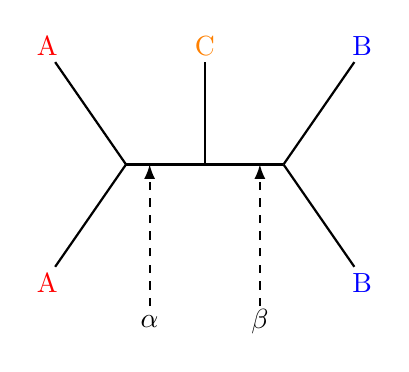
\begin{tikzpicture}
    \node[red] at (0,0) {A};
    \node[red] at (0,3) {A};
    \node[blue] at (4,0) {B};
    \node[blue] at (4,3) {B};
    \node[orange] at (2,3) {C};
    \draw [black,thick](0.1,0.2) -- (1,1.5);
    \draw [black,thick](0.1,2.8) -- (1,1.5);
    \draw [black,thick](1,1.5) -- (3,1.5);
    \draw [black,thick](3.9,0.2) -- (3,1.5);
    \draw [black,thick](3.9,2.8) -- (3,1.5);
    \draw [black,thick](2,1.5) -- (2,2.8);
    \draw [-latex,black,thick,dashed](1.3,-0.3)--(1.3,1.5);
    \draw [-latex,black,thick,dashed](2.7,-0.3)--(2.7,1.5);
    \node[black] at (1.3,-0.5) {$\alpha$};
    \node[black] at (2.7,-0.5) {$\beta$};
\end{tikzpicture}
\end{center}
\caption{Tree 1}
\end{subfigure}
\begin{subfigure}[b]{0.3\textwidth}
\begin{center}
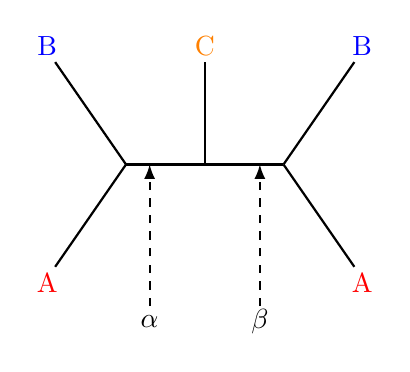
\begin{tikzpicture}
    \node[red] at (0,0) {A};
    \node[red] at (4,0) {A};
    \node[blue] at (0,3) {B};
    \node[blue] at (4,3) {B};
    \node[orange] at (2,3) {C};
    \draw [black,thick](0.1,0.2) -- (1,1.5);
    \draw [black,thick](0.1,2.8) -- (1,1.5);
    \draw [black,thick](1,1.5) -- (3,1.5);
    \draw [black,thick](3.9,0.2) -- (3,1.5);
    \draw [black,thick](3.9,2.8) -- (3,1.5);
    \draw [black,thick](2,1.5) -- (2,2.8);
    \draw [-latex,black,thick,dashed](1.3,-0.3)--(1.3,1.5);
    \draw [-latex,black,thick,dashed](2.7,-0.3)--(2.7,1.5);
    \node[black] at (1.3,-0.5) {$\alpha$};
    \node[black] at (2.7,-0.5) {$\beta$};
\end{tikzpicture}
\end{center}
\caption{Tree 2}
\end{subfigure}
\begin{subfigure}[b]{0.3\textwidth}
\begin{center}
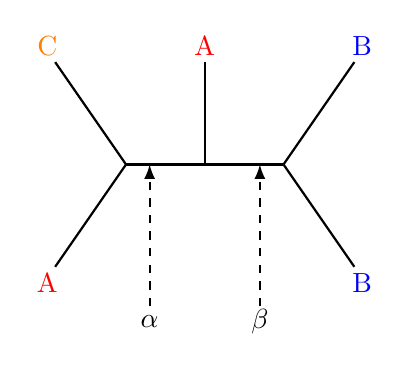
\begin{tikzpicture}
    \node[red] at (0,0) {A};
    \node[red] at (2,3) {A};
    \node[blue] at (4,0) {B};
    \node[blue] at (4,3) {B};
    \node[orange] at (0,3) {C};
    \draw [black,thick](0.1,0.2) -- (1,1.5);
    \draw [black,thick](0.1,2.8) -- (1,1.5);
    \draw [black,thick](1,1.5) -- (3,1.5);
    \draw [black,thick](3.9,0.2) -- (3,1.5);
    \draw [black,thick](3.9,2.8) -- (3,1.5);
    \draw [black,thick](2,1.5) -- (2,2.8);
    \draw [-latex,black,thick,dashed](1.3,-0.3)--(1.3,1.5);
    \draw [-latex,black,thick,dashed](2.7,-0.3)--(2.7,1.5);
    \node[black] at (1.3,-0.5) {$\alpha$};
    \node[black] at (2.7,-0.5) {$\beta$};
\end{tikzpicture}
\end{center}
\caption{Tree 3}
\end{subfigure}
\vspace{0.5cm}
\caption{Illustrative examples of the topological compatibility measurement. Three trees with $5$ leaves are given, and $2$ of the leaves belong to group A, $2$ of the leaves belong to B, while only one leaf belong to group C.}
\label{fig:topologicaltree}
\end{figure}

\section{Additional Figures and Tables to the Main Text}
In this section, we provide FIG. \ref{fig:JC01Mb}, FIG. \ref{fig:GTR01Mb}, and FIG. \ref{fig:Geno2DSFSNGSDistDepth}, as well as Table \ref{tab:ConsensusGT01M} as additional figures and tables of the main text.
\begin{table*}[h]
    \centering
    \begin{tabular}{|c|c|c|c|c|c|c|c|}
     \hline
      \multirow{3}{*}{Average Read Depth} & \multirow{3}{*}{Variable Genome Length(Mb)} & \multicolumn{6}{c|}{Mean of Inferred $\hat{d}$}\\
      &&\multicolumn{2}{c|}{True $d$: $0.8000$}&\multicolumn{2}{c|}{True $d$: $1.000$}&\multicolumn{2}{c|}{True $d$: $1.600$}\\
      &&JC69&GTR&JC69&GTR&JC69&GTR\\
      \hline
      $20$ & $0.1$ & $0.3147$ & $0.3124$ & $0.5118$ & $0.4866$ & $1.105$ & $1.012$\\
      \hline
      $10$ & $0.1$ & $0.3228$ & $0.3207$ & $0.5204$ & $0.4957$ & $1.114$ & $1.020$\\
      \hline
      $5$ & $0.1$ & $0.3941$ & $0.3953$ & $0.5922$ & $0.5722$ & $1.188$ & $1.107$\\
      \hline
      $1$ & $0.1$ & $0.6903$ & $0.6998$ & $0.8912$ & $0.8911$ & $1.493$ & $1.482$\\
       \hline
     $0.75$ & $0.1$ & $0.7174$ & $0.7274$ & $0.9195$ & $0.9245$ & $1.520$ & $1.520$\\
      \hline
      $0.5$ & $0.1$ & $0,7475$ & $0.7579$ & $0,9478$ & $0.9599$ & $1,547$ & $1.561$\\
      \hline
      \end{tabular}
    \caption{ConsensusGT inferred results based on 200 replicates of simulations of different models.}
    \label{tab:ConsensusGT01M}
\end{table*}

\begin{figure*}[h]
    \centering
    \begin{subfigure}[b]{0.475\textwidth}
         \centering
         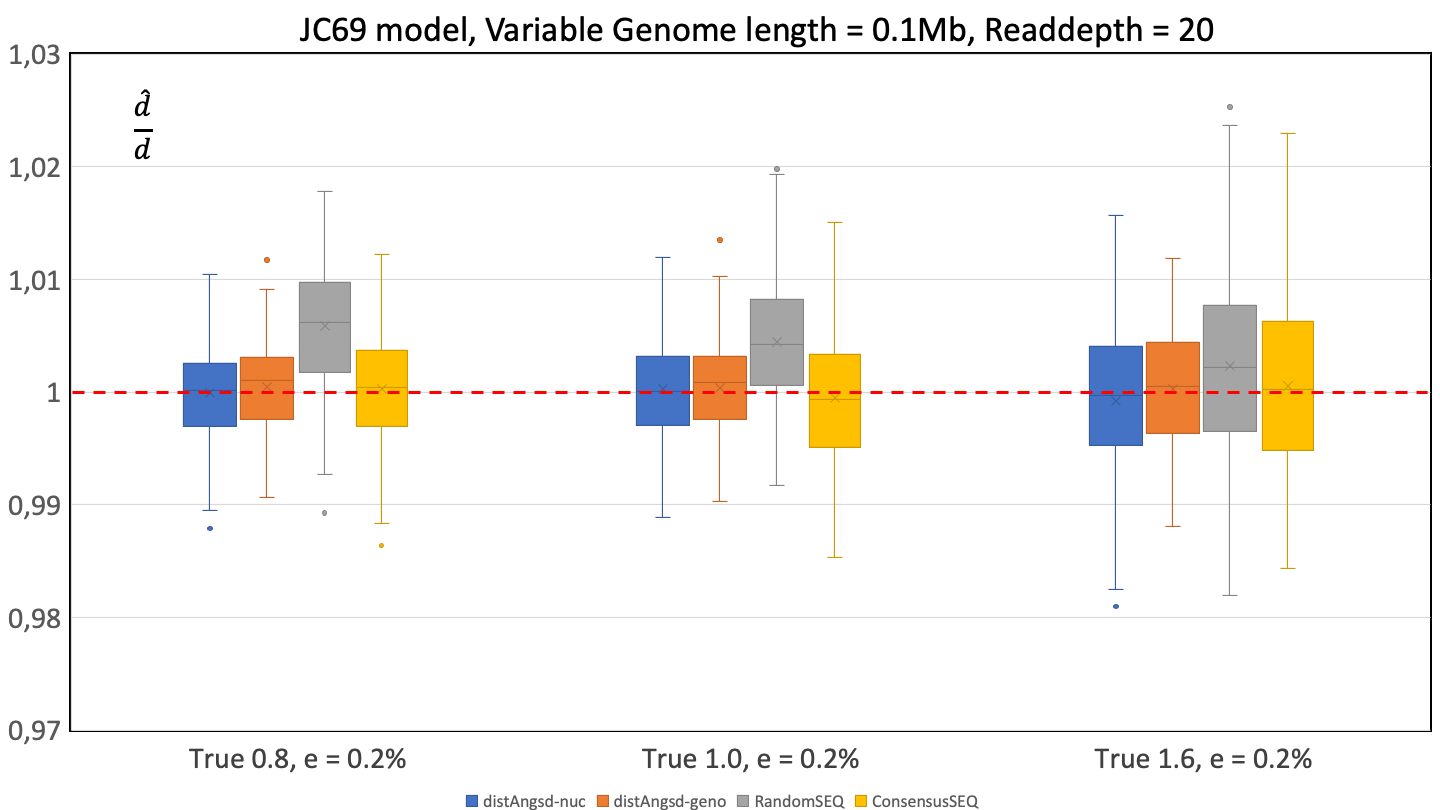
\includegraphics[width=\textwidth]{JCRD20_01Mb.png}
         \caption{}
         \label{fig:JCRD20_01Mb}
     \end{subfigure}
     \begin{subfigure}[b]{0.475\textwidth}
         \centering
         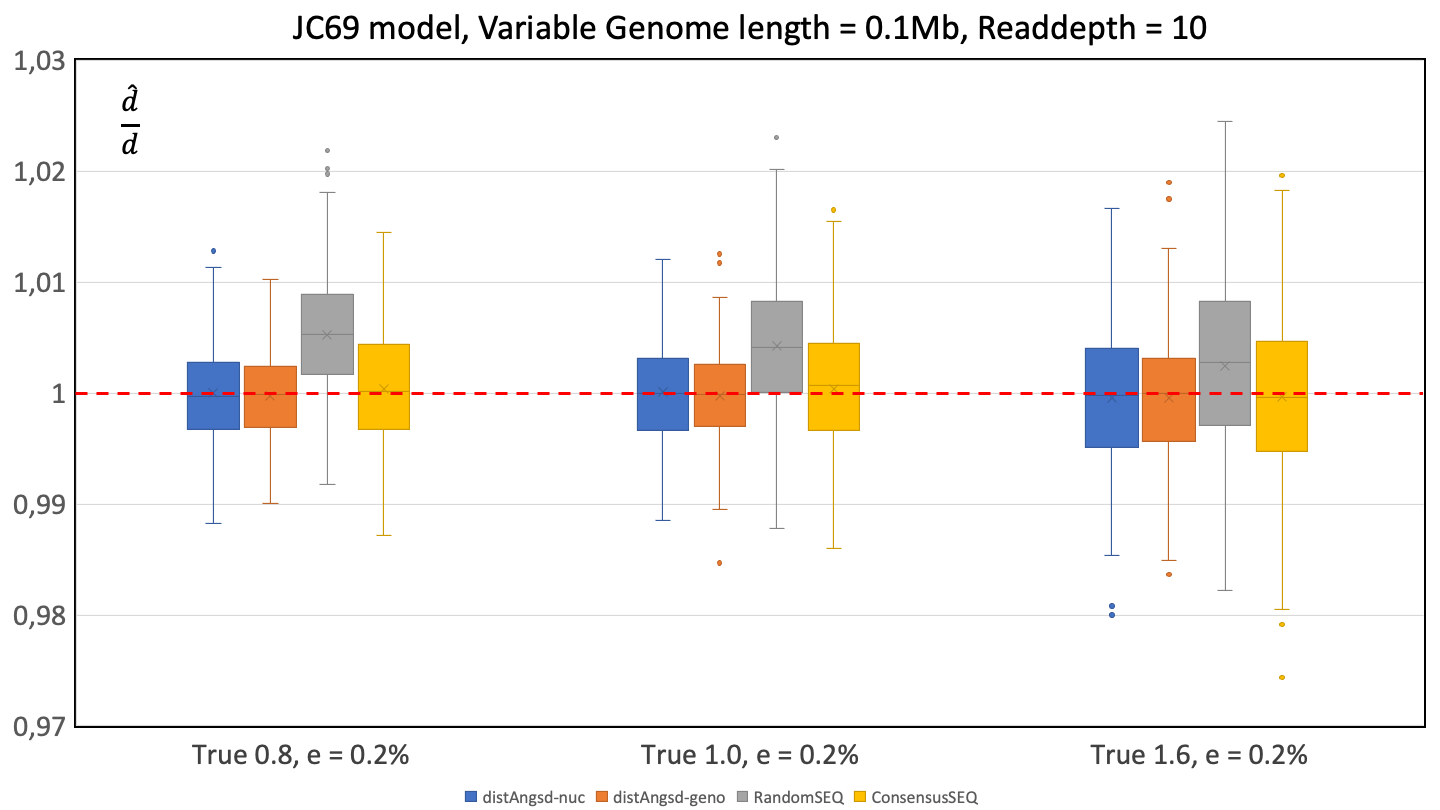
\includegraphics[width=\textwidth]{JCRD10_01Mb.png}
         \caption{}
         \label{fig:JCRD10_01Mb}
     \end{subfigure}
     \begin{subfigure}[b]{0.475\textwidth}
         \centering
         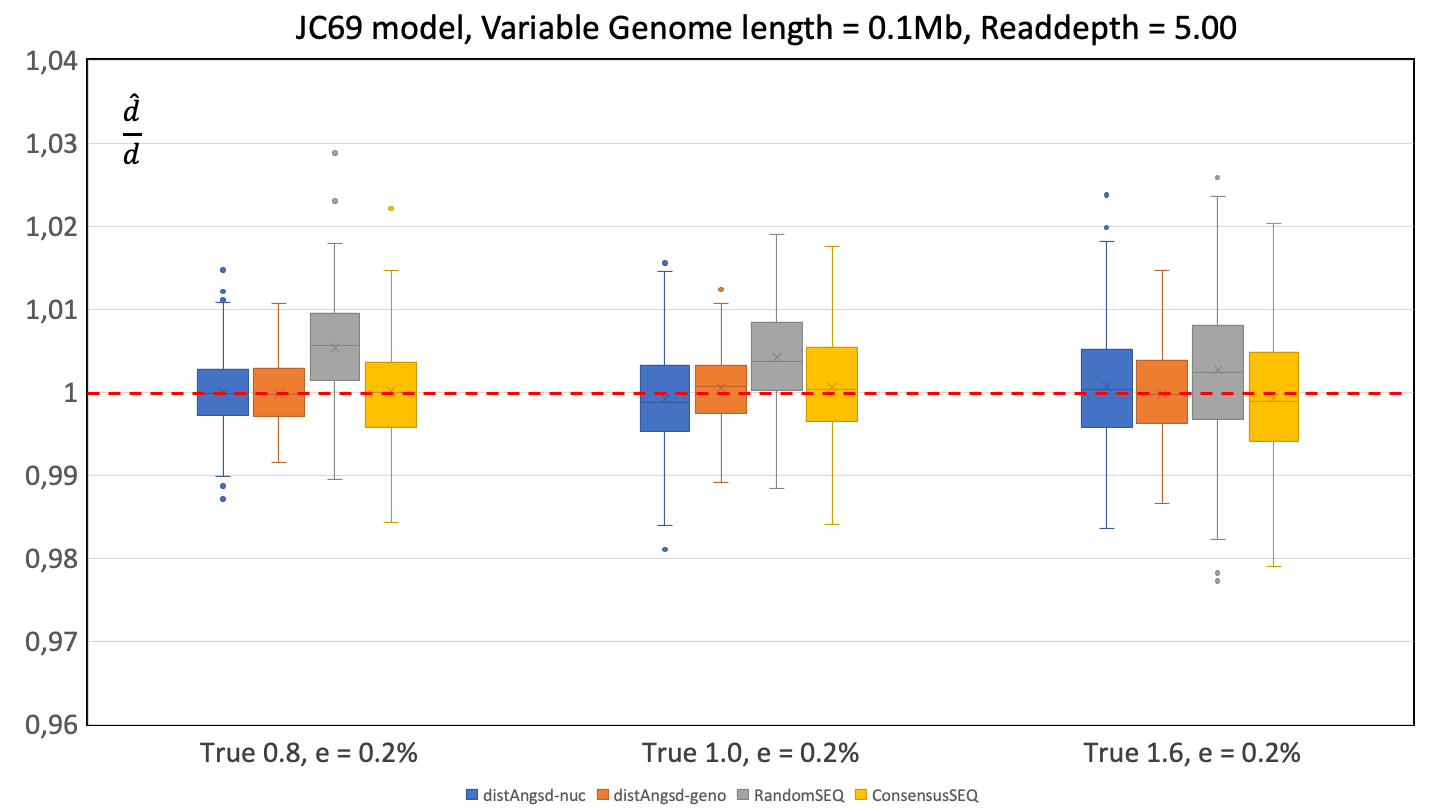
\includegraphics[width=\textwidth]{JCRD5_01Mb.png}
         \caption{}
         \label{fig:JCRD5_01Mb}
     \end{subfigure}
     \begin{subfigure}[b]{0.475\textwidth}
         \centering
         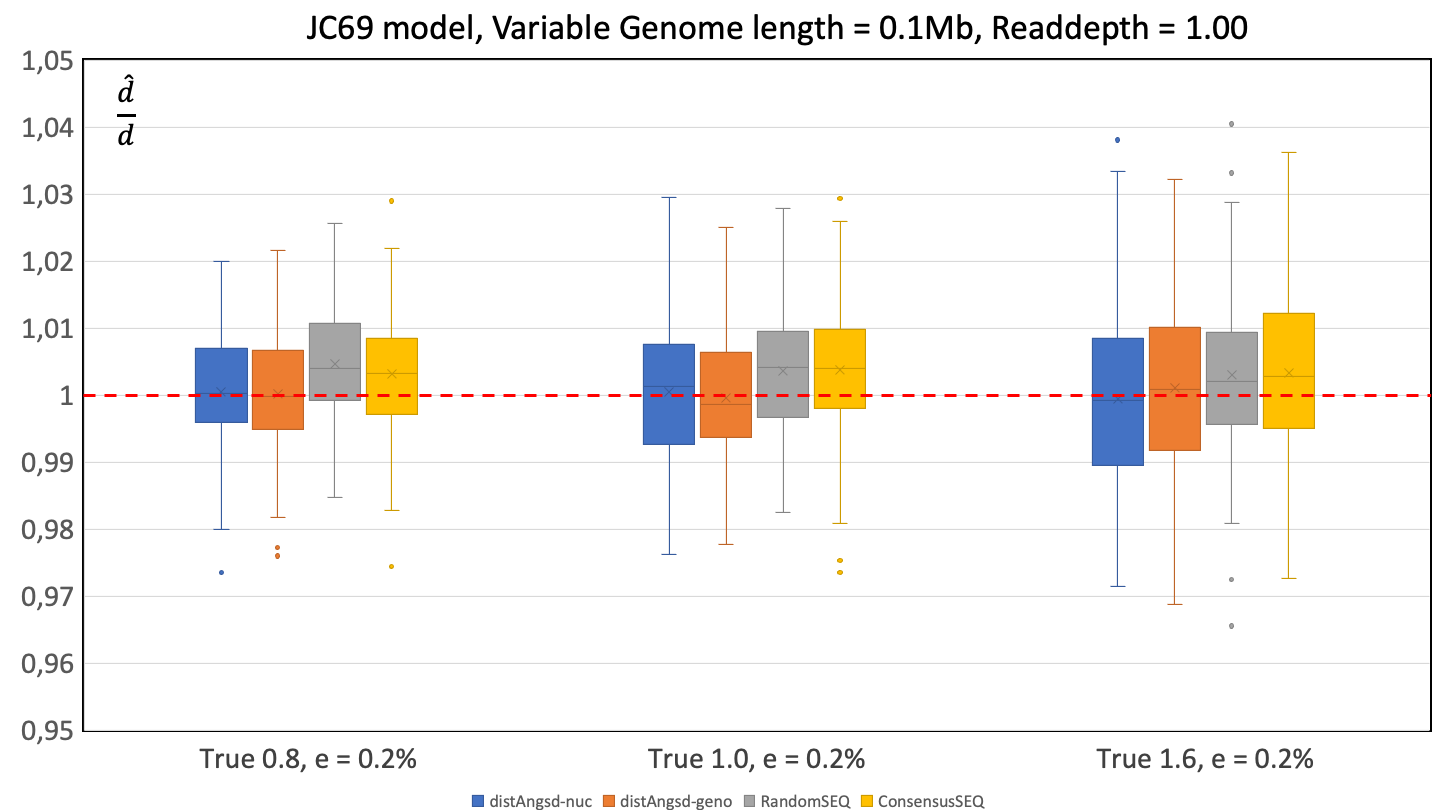
\includegraphics[width=\textwidth]{JCRD1_01Mb.png}
         \caption{}
         \label{fig:JCRD1_01Mb}
     \end{subfigure}
     \begin{subfigure}[b]{0.475\textwidth}
         \centering
         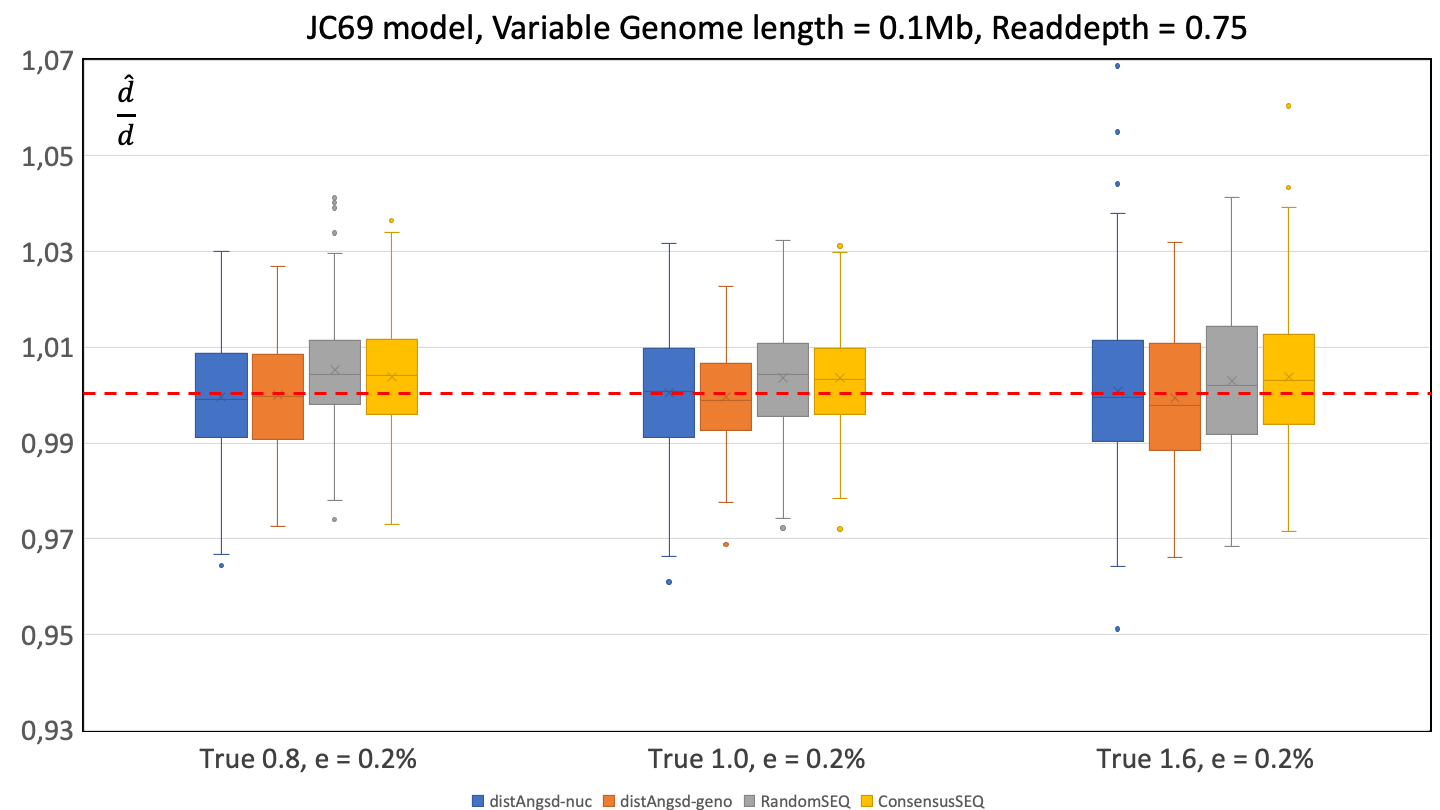
\includegraphics[width=\textwidth]{JCRD075_01Mb.png}
         \caption{}
         \label{fig:JCRD075_01Mb}
    \end{subfigure}
     \begin{subfigure}[b]{0.475\textwidth}
         \centering
         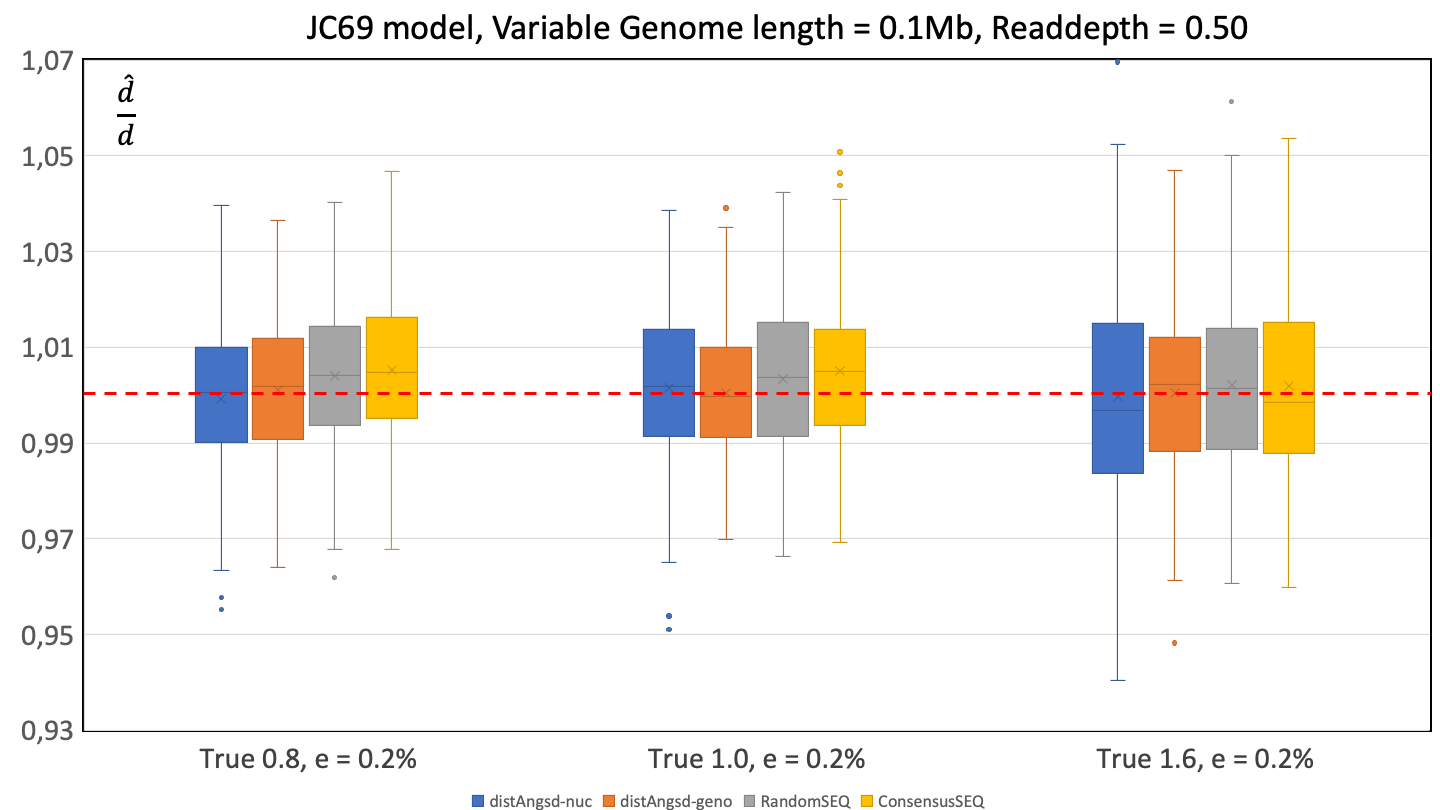
\includegraphics[width=\textwidth]{JCRD05_01Mb.png}
         \caption{}
         \label{fig:JCRD05_01Mb}
    \end{subfigure}
    \vspace{0.5cm}
    \caption{The inferred results of four different methods based $200$ replicates of JC69 model simulation, i.e., distAngsd-nuc, distAngsd-geno, RandomSEQ, and ConsensusSEQ when genome length is $0.1$Mb, and the average read depth per site varies from (a) $20$ to (f) $0.5$. The simulated base calling error is $e =0.2\%$. Simulated divergence tree follows FIG. 1 in the main text, with $t_1=0.4$ and $t_2 = 0.25$, and true simulated divergence time $t$ (hence the genetic distance $d$) is set as $0.8$, $1.0$ and $1.6$.}
    \label{fig:JC01Mb}
\end{figure*}

\begin{figure*}[h]
    \centering
        \begin{subfigure}[b]{0.475\textwidth}
         \centering
         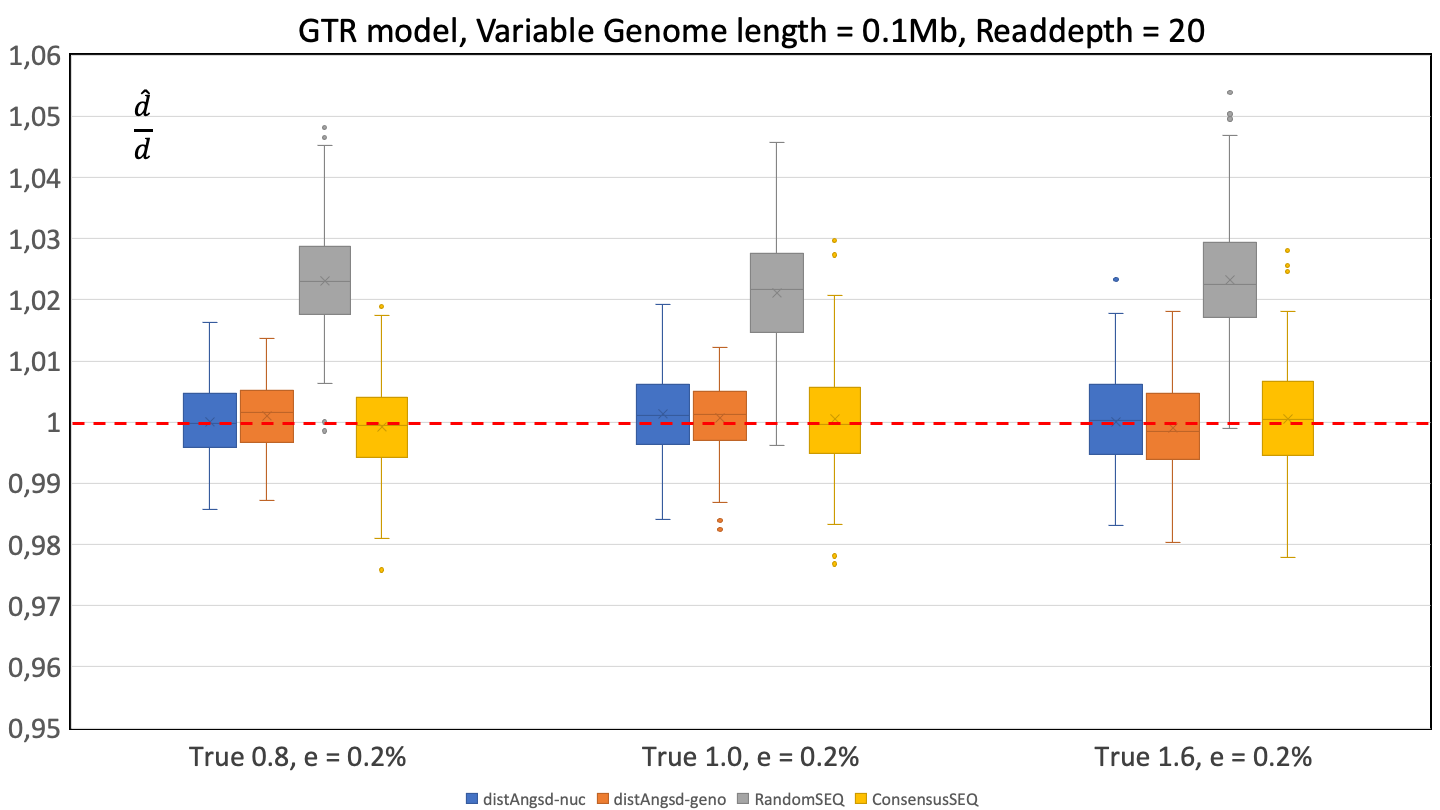
\includegraphics[width=\textwidth]{GTRRD20_01Mb.png}
         \caption{}
         \label{fig:GTRRD20_01Mb}
     \end{subfigure}
     \begin{subfigure}[b]{0.475\textwidth}
         \centering
         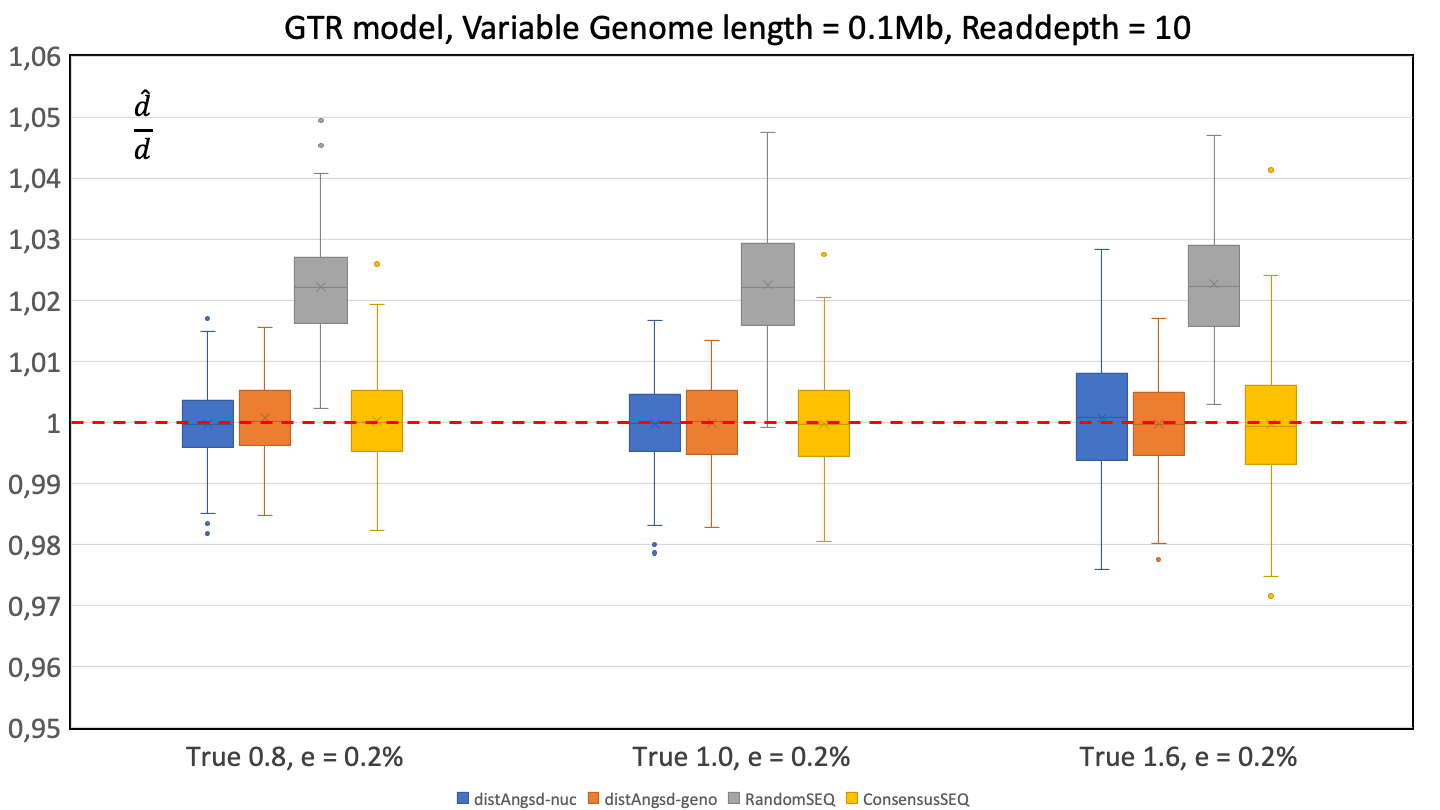
\includegraphics[width=\textwidth]{GTRRD10_01Mb.png}
         \caption{}
         \label{fig:GTRRD10_01Mb}
     \end{subfigure}
     \begin{subfigure}[b]{0.475\textwidth}
         \centering
         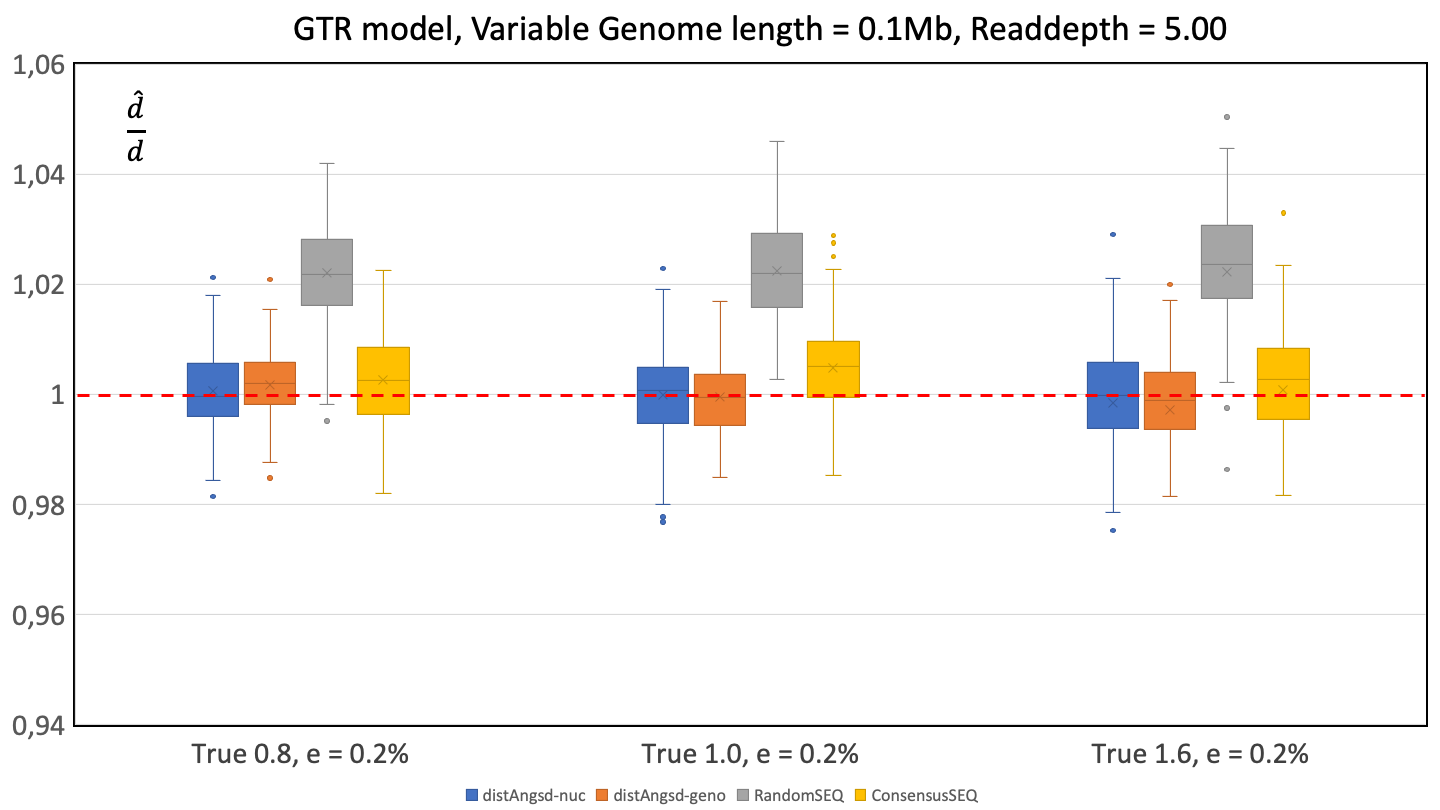
\includegraphics[width=\textwidth]{GTRRD5_01Mb.png}
         \caption{}
         \label{fig:GTRRD5_01Mb}
     \end{subfigure}
     \begin{subfigure}[b]{0.475\textwidth}
         \centering
         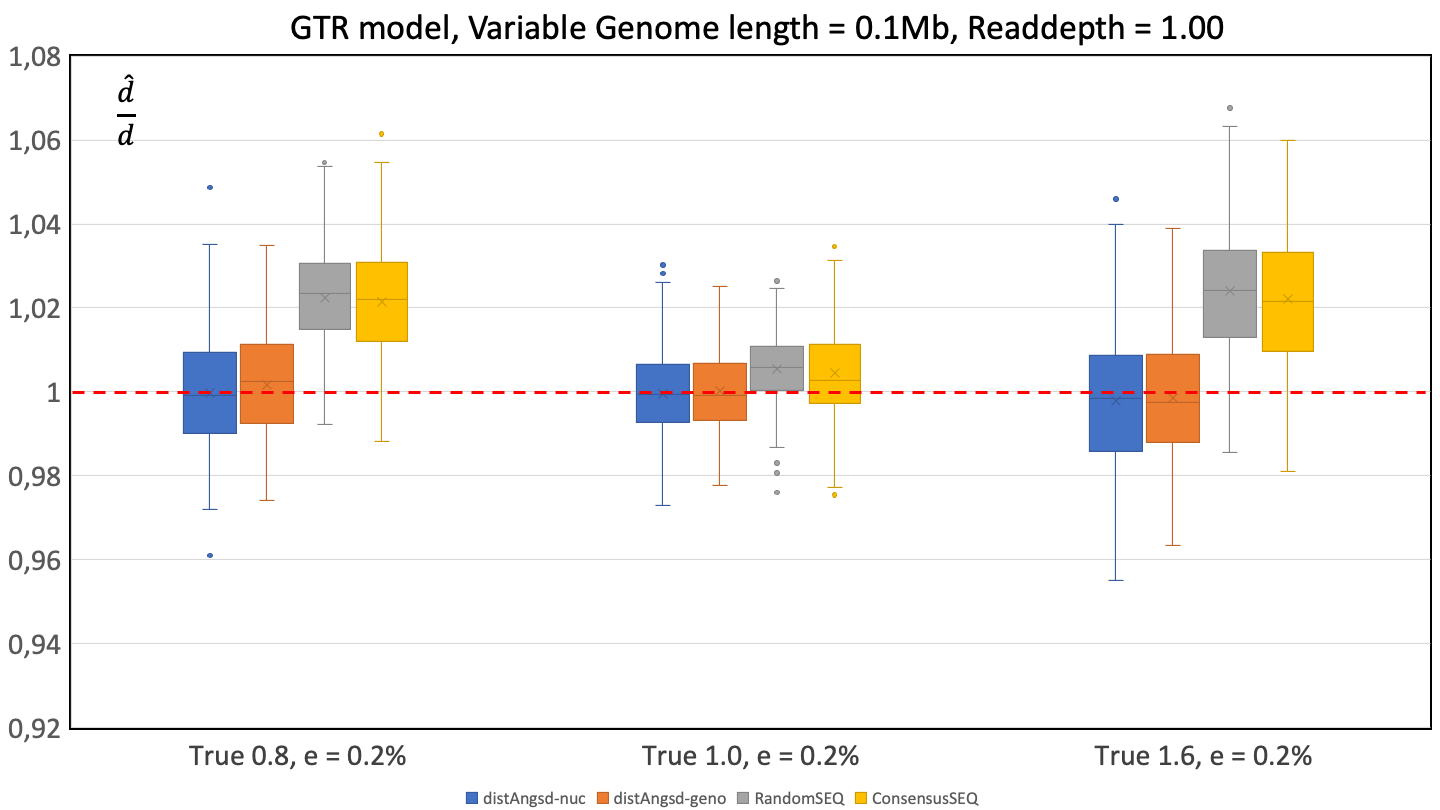
\includegraphics[width=\textwidth]{GTRRD1_01Mb.png}
         \caption{}
         \label{fig:GTRRD1_01Mb}
     \end{subfigure}
     \begin{subfigure}[b]{0.475\textwidth}
         \centering
         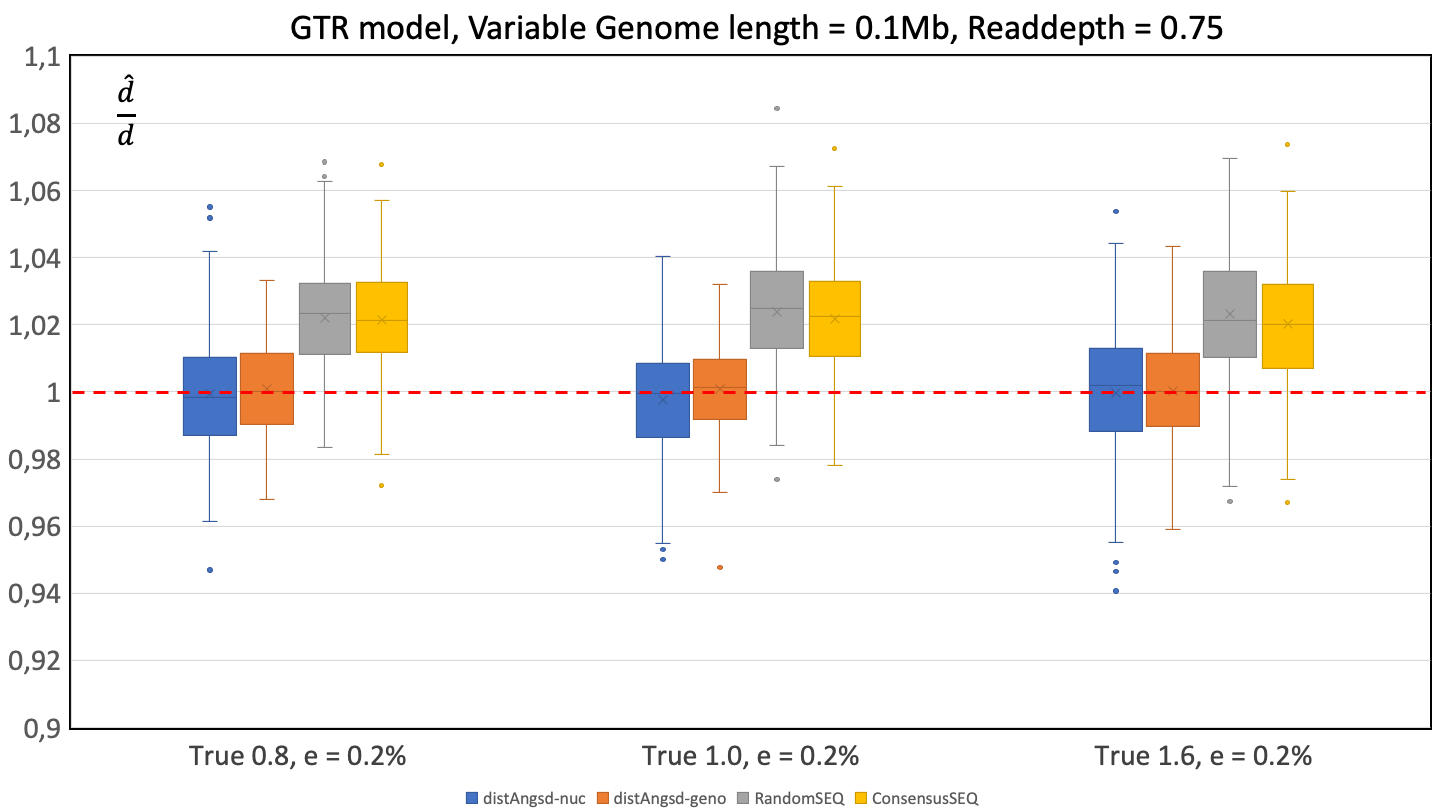
\includegraphics[width=\textwidth]{GTRRD075_01Mb.png}
         \caption{}
         \label{fig:GTRRD075_01Mb}
     \end{subfigure}
     \begin{subfigure}[b]{0.475\textwidth}
         \centering
         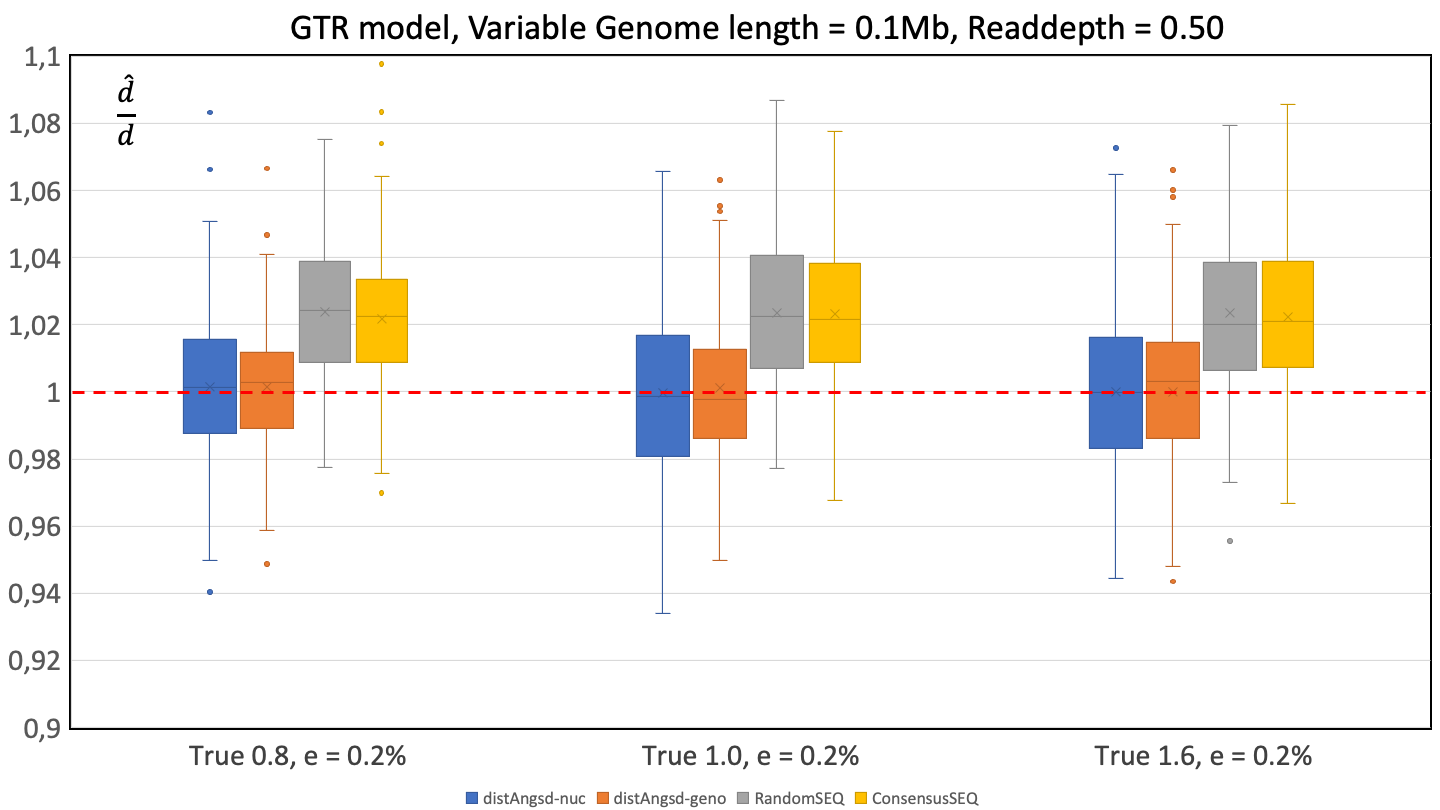
\includegraphics[width=\textwidth]{GTRRD05_01Mb.png}
         \caption{}
         \label{fig:GTRRD05_01Mb}
     \end{subfigure}
    \vspace{0.5cm}
    \caption{The inferred results of four different methods based $200$ replicates of GTR model simulation, i.e., distAngsd-nuc, distAngsd-geno, RandomSEQ, and ConsensusSEQ when genome length is $0.1$Mb, and the average read depth per site varies from (a) $20$ to (f) $0.5$. The simulated base calling error is $e =0.2\%$. Simulated divergence tree follows FIG. 1 in the main text, with $t_1=0.4$ and $t_2 = 0.25$, and true simulated divergence time $t$ (hence the genetic distance $d$) is set as $0.8$, $1.0$ and $1.6$.}
    \label{fig:GTR01Mb}
\end{figure*}

% \begin{table*}[ht]
%     \centering
%     \begin{tabular}{|c|c|c|c|c|c|c|c|}
%      \hline
%       \multirow{3}{*}{Average Read Depth} & \multirow{3}{*}{Variable Genome Length(Mb)} & \multicolumn{6}{c|}{Inferred $\hat{d}$}\\
%       &&\multicolumn{2}{c|}{True $d$: $0.8000$}&\multicolumn{2}{c|}{True $d$: $1.000$}&\multicolumn{2}{c|}{True $d$: $1.600$}\\
%       &&JC69&GTR&JC69&GTR&JC69&GTR\\
%       \hline
%       \multirow{2}{*}{$20$} & $0.1$ & $0.3147$ & $0.3124$ & $0.5118$ & $0.4866$ & $1.105$ & $1.012$\\
%       & $1$ & $0.3149$ &$0.3119$& $0.5122$ & $0.4870$ & $1.105$ & $1.011$\\
%       \hline
%       \multirow{2}{*}{$10$} & $0.1$ & $0.3228$ & $0.3207$ & $0.5204$ & $0.4957$ & $1.114$ & $1.020$\\
%       & $1$ & $0.3229$ & $0.3206$ & $0.5204$ & $0.4957$ & $1.114$ & $1.020$\\
%       \hline
%       \multirow{2}{*}{$5$} & $0.1$ & $0.3941$ & $0.3953$ & $0.5922$ & $0.5722$ & $1.188$ & $1.107$\\
%       & $1$ & $0.3941$ & $0.3949$ & $0.5926$ & $0.5725$ & $1.188$ & $1.107$\\
%       \hline
%       \multirow{2}{*}{$1$} & $0.1$ & $0.6903$ & $0.6998$ & $0.8912$ & $0.8911$ & $1.493$ & $1.482$\\
%       & $1$ & $0.6900$ & $0.6983$ & $0.8907$ & $0.8931$ & $1.492$ & $1.480$\\
%       \hline
%       \multirow{2}{*}{$0.75$} & $0.1$ & $0.7174$ & $0.7274$ & $0.9195$ & $0.9245$ & $1.520$ & $1.520$\\
%       & $1$ & $0.7180$ & $0.7265$ & $0.9186$ & $0.9246$ & $0.9186$ & $1.517$\\
%       \hline
%       \multirow{2}{*}{$0.5$} & $0.1$ & $0,7475$ & $0.7579$ & $0,9478$ & $0.9599$ & $1,547$ & $1.561$\\
%       & $1$ & $0.7459$ & $0.7571$ & $0.9465$ & $0.9565$ & $1.548$ & $1.557$\\
%       \hline
%       \end{tabular}
%     \caption{ConsensusGT inferred results based on 200 replicates of simulations of different models.}
%     \label{tab:ConsensusGT}
% \end{table*}

\begin{figure*}[h]
    \centering
        \begin{subfigure}[b]{0.475\textwidth}
         \centering
         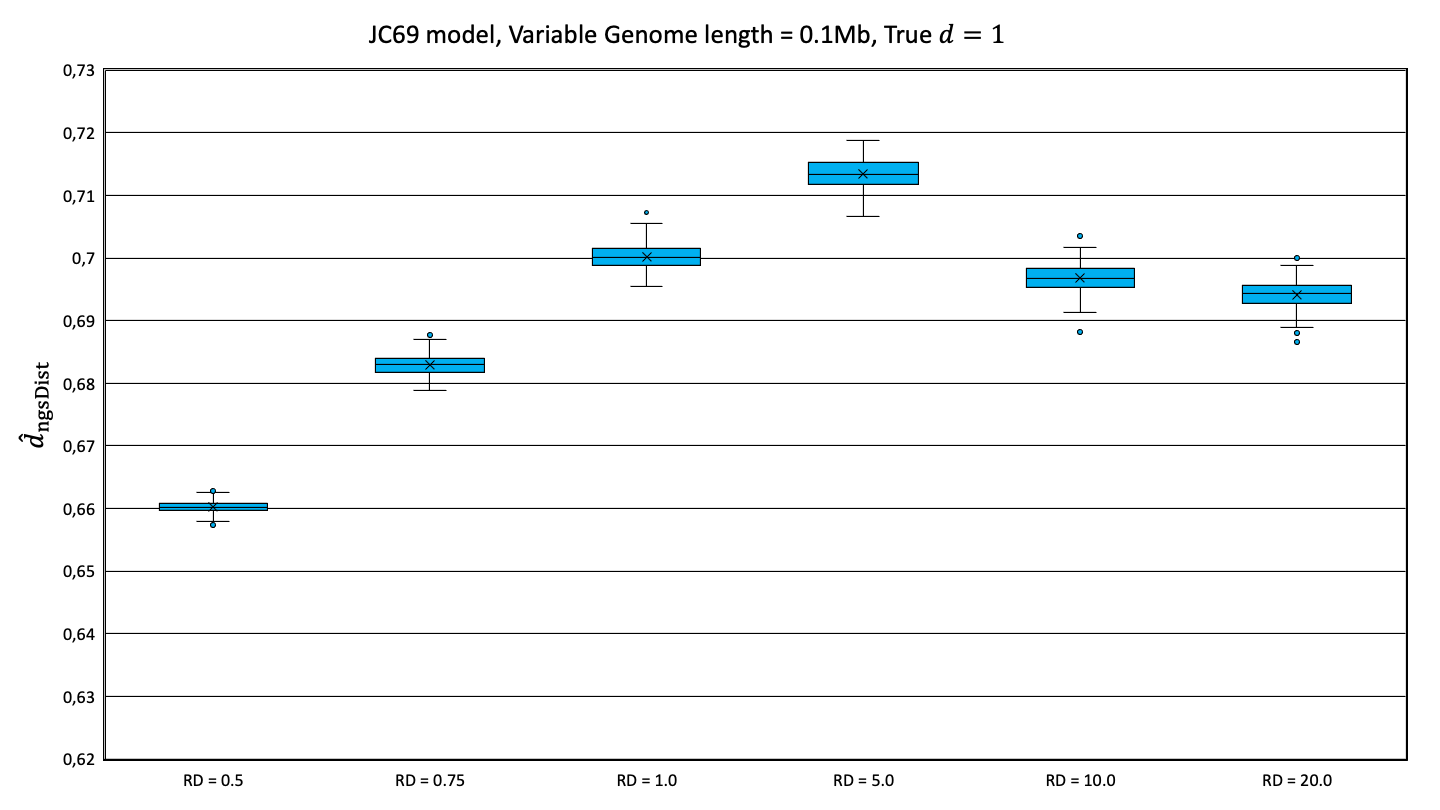
\includegraphics[width=\textwidth]{NGSdist01Mb.png}
         \caption{}
         \label{fig:NGSdistRD01Mb}
     \end{subfigure}
     \begin{subfigure}[b]{0.475\textwidth}
         \centering
         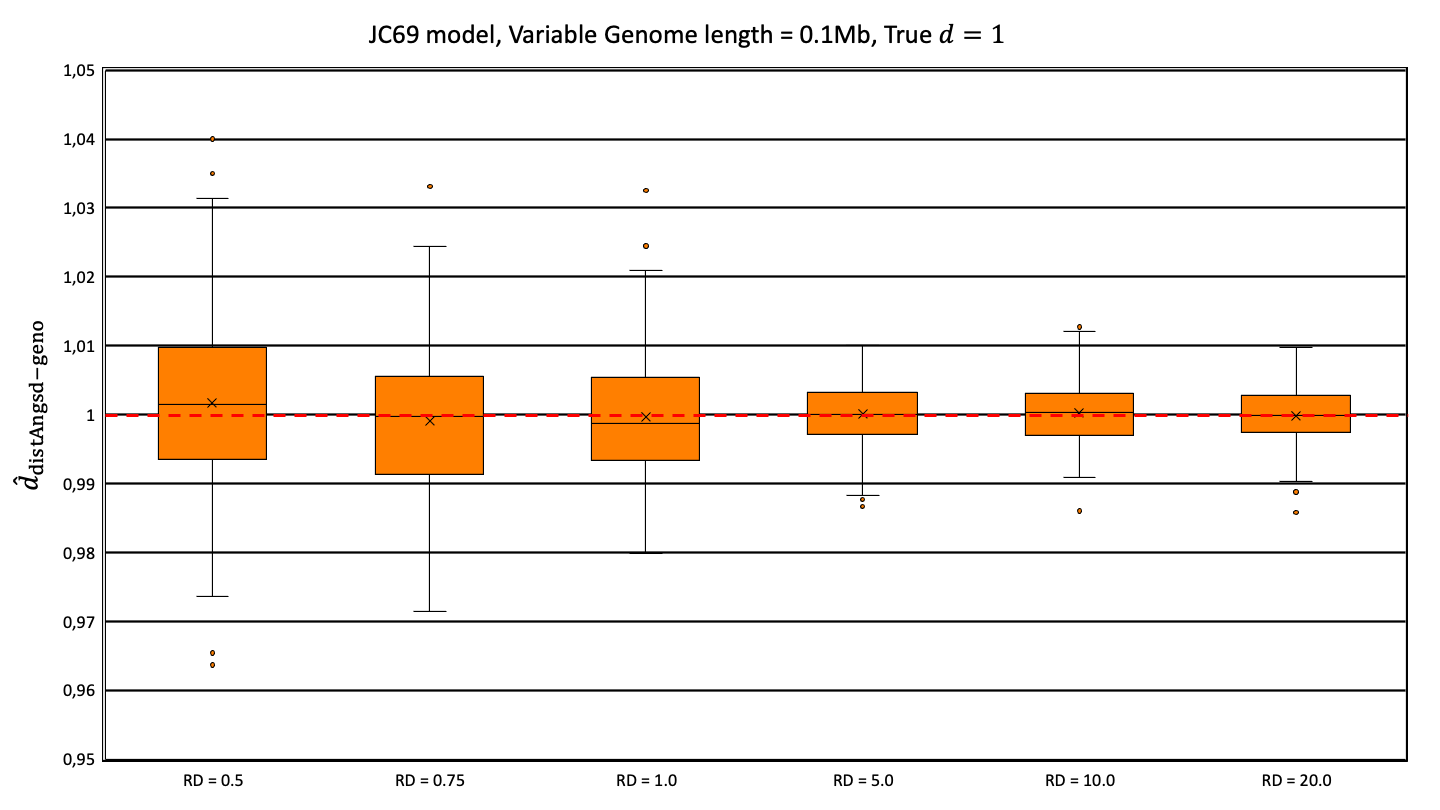
\includegraphics[width=\textwidth]{distAngsd-geno01Mb.png}
         \caption{}
         \label{fig:distAngsd-genoRD01Mb}
     \end{subfigure}
        \begin{subfigure}[b]{0.475\textwidth}
         \centering
         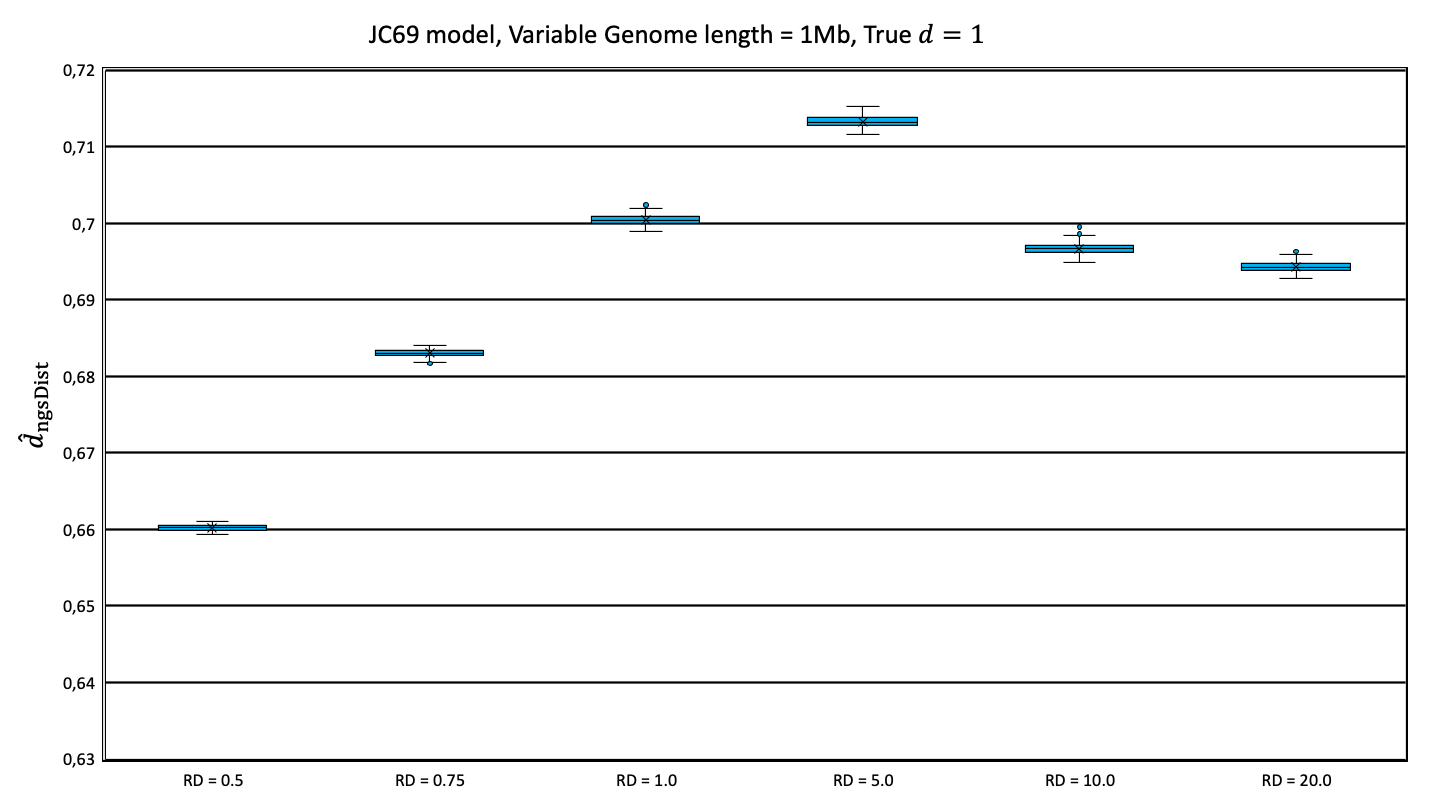
\includegraphics[width=\textwidth]{NGSdist.png}
         \caption{}
         \label{fig:NGSdist}
     \end{subfigure}
     \begin{subfigure}[b]{0.475\textwidth}
         \centering
         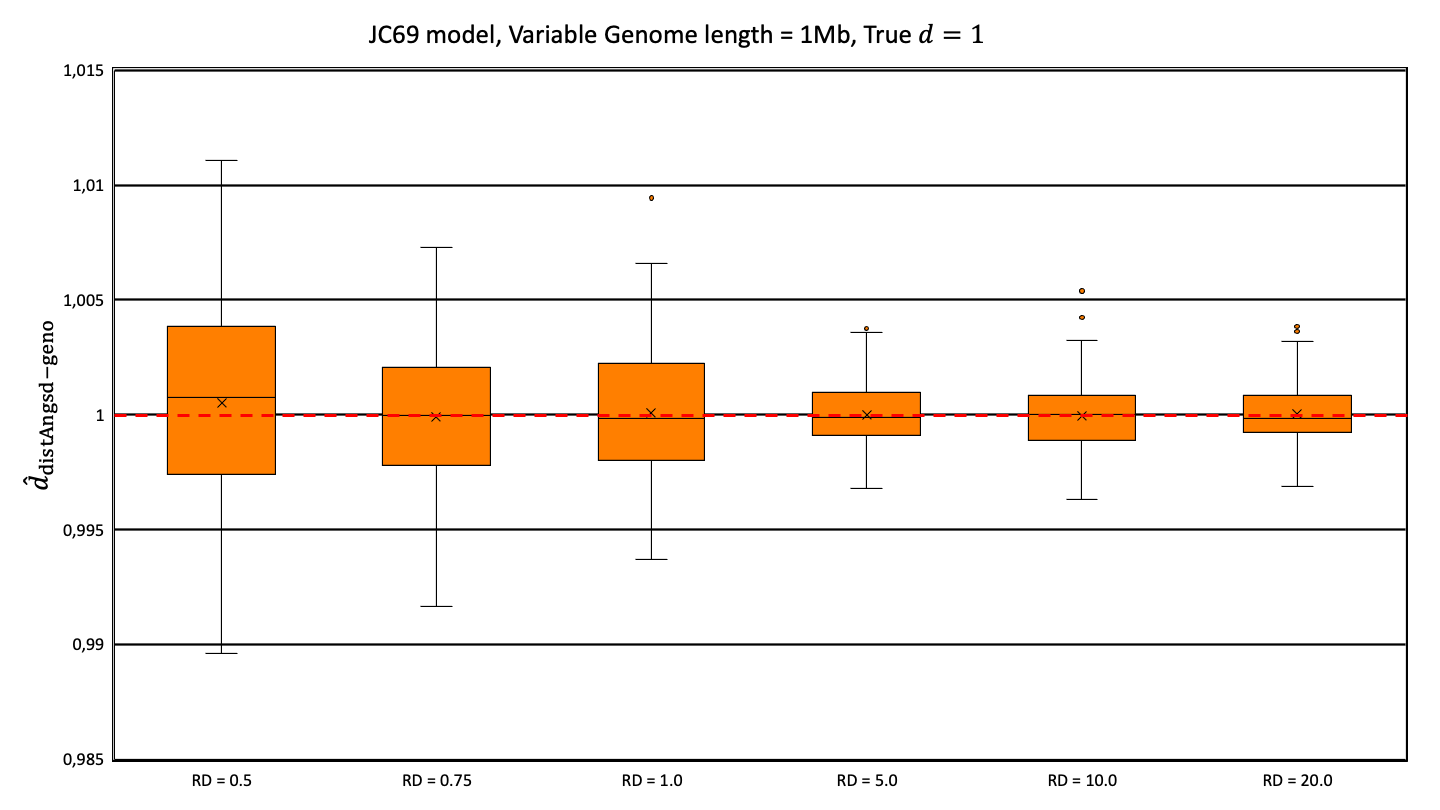
\includegraphics[width=\textwidth]{distAngsd-geno.png}
         \caption{}
         \label{fig:distAngsd-geno}
     \end{subfigure}
    \vspace{0.5cm}
    \caption{JC69 model is simulated to compare the inference results of distAngsd-geno and ngsDist with different read depths, $20$, $10$, $5$, $1$, $0.75$ and $0.5$ and same true genetic distance $d=1$ (follows divergence tree as FIG. 1 in the main text, with $t_1=0.4$ and $t_2 = 0.25$). Simulated genome lengths $1$Mb (a)(b) and $0.1$Mb (c)(d) are considered. With genotype likelihoods taken into account, The estimates of both ngsDist and distAngsd-geno were expected to fluctuated around some certain value as genome length varies. But ngsDist will not stay the same which is due to limited information of genotype likelihoods are used.}
    \label{fig:Geno2DSFSNGSDistDepth}
\end{figure*}
\bibliographystyle{unsrtnat}
\bibliography{refs}
\end{document} 